%% Run LaTeX on this file several times to get Table of Contents,
%% cross-references, and citations.

\documentclass[11pt]{book}
\usepackage{gvv}
\usepackage{gvv-book-bkup}
%\usepackage{Wiley-AuthoringTemplate}
\usepackage[sectionbib,authoryear]{natbib}% for name-date citation comment the below line
%\usepackage[sectionbib,numbers]{natbib}% for numbered citation comment the above line

%%********************************************************************%%
%%       How many levels of section head would you like numbered?     %%
%% 0= no section numbers, 1= section, 2= subsection, 3= subsubsection %%
\setcounter{secnumdepth}{3}
%%********************************************************************%%
%%**********************************************************************%%
%%     How many levels of section head would you like to appear in the  %%
%%				Table of Contents?			%%
%% 0= chapter, 1= section, 2= subsection, 3= subsubsection titles.	%%
\setcounter{tocdepth}{2}
%%**********************************************************************%%
\setcounter{tocdepth}{3}
%\includeonly{ch01}
\makeindex

\begin{document}

\frontmatter
%%%%%%%%%%%%%%%%%%%%%%%%%%%%%%%%%%%%%%%%%%%%%%%%%%%%%%%%%%%%%%%%
%% Title Pages
%% Wiley will provide title and copyright page, but you can make
%% your own titlepages if you'd like anyway
%% Setting up title pages, type in the appropriate names here:

\booktitle{CBSE Math}

\subtitle{Made Simple}

\AuAff{G. V. V. Sharma}

%% \\ will start a new line.
%% You may add \affil{} for affiliation, ie,
%\authors{Robert M. Groves\\
%\affil{Universitat de les Illes Balears}
%Floyd J. Fowler, Jr.\\
%\affil{University of New Mexico}
%}

%% Print Half Title and Title Page:
%\halftitlepage
\titlepage

%%%%%%%%%%%%%%%%%%%%%%%%%%%%%%%%%%%%%%%%%%%%%%%%%%%%%%%%%%%%%%%%
%%Copyright Page

\begin{copyrightpage}{2023}
%Title, etc
\end{copyrightpage}

% Note, you must use \ to start indented lines, ie,
% 
% \begin{copyrightpage}{2004}
% Survey Methodology / Robert M. Groves . . . [et al.].
% \       p. cm.---(Wiley series in survey methodology)
% \    ``Wiley-Interscience."
% \    Includes bibliographical references and index.
% \    ISBN 0-471-48348-6 (pbk.)
% \    1. Surveys---Methodology.  2. Social 
% \  sciences---Research---Statistical methods.  I. Groves, Robert M.  II. %
% Series.\\

% HA31.2.S873 2004
% 001.4'33---dc22                                             2004044064
% \end{copyrightpage}

%%%%%%%%%%%%%%%%%%%%%%%%%%%%%%%%%%%%%%%%%%%%%%%%%%%%%%%%%%%%%%%%
%% Only Dedication (optional) 

%\dedication{To my parents}

\tableofcontents

%\listoffigures %optional
%\listoftables  %optional

%% or Contributor Page for edited books
%% before \tableofcontents

%%%%%%%%%%%%%%%%%%%%%%%%%%%%%%%%%%%%%%%%%%%%%%%%%%%%%%%%%%%%%%%%
%  Contributors Page for Edited Book
%%%%%%%%%%%%%%%%%%%%%%%%%%%%%%%%%%%%%%%%%%%%%%%%%%%%%%%%%%%%%%%%

% If your book has chapters written by different authors,
% you'll need a Contributors page.

% Use \begin{contributors}...\end{contributors} and
% then enter each author with the \name{} command, followed
% by the affiliation information.

% \begin{contributors}
% \name{Masayki Abe,} Fujitsu Laboratories Ltd., Fujitsu Limited, Atsugi, Japan
%
% \name{L. A. Akers,} Center for Solid State Electronics Research, Arizona State University, Tempe, Arizona
%
% \name{G. H. Bernstein,} Department of Electrical and Computer Engineering, University of Notre Dame, Notre Dame, South Bend, Indiana; formerly of
% Center for Solid State Electronics Research, Arizona
% State University, Tempe, Arizona 
% \end{contributors}

%%%%%%%%%%%%%%%%%%%%%%%%%%%%%%%%%%%%%%%%%%%%%%%%%%%%%%%%%%%%%%%%
% Optional Foreword:

%\begin{foreword}
%\lipsum[1-2]
%\end{foreword}

%%%%%%%%%%%%%%%%%%%%%%%%%%%%%%%%%%%%%%%%%%%%%%%%%%%%%%%%%%%%%%%%
% Optional Preface:

%\begin{preface}
%\lipsum[1-1]
%\prefaceauthor{}
%\where{place\\
% date}
%\end{preface}

% ie,
% \begin{preface}
% This is an example preface.
% \prefaceauthor{R. K. Watts}
% \where{Durham, North Carolina\\
% September, 2004}

%%%%%%%%%%%%%%%%%%%%%%%%%%%%%%%%%%%%%%%%%%%%%%%%%%%%%%%%%%%%%%%%
% Optional Acknowledgments:

%\acknowledgments
%\lipsum[1-2]
%\authorinitials{I. R. S.}  

%%%%%%%%%%%%%%%%%%%%%%%%%%%%%%%%
%% Glossary Type of Environment:

% \begin{glossary}
% \term{<term>}{<description>}
% \end{glossary}

%%%%%%%%%%%%%%%%%%%%%%%%%%%%%%%%
%\begin{acronyms}
%\acro{ASTA}{Arrivals See Time Averages}
%\acro{BHCA}{Busy Hour Call Attempts}
%\acro{BR}{Bandwidth Reservation}
%\acro{b.u.}{bandwidth unit(s)}
%\acro{CAC}{Call / Connection Admission Control}
%\acro{CBP}{Call Blocking Probability(-ies)}
%\acro{CCS}{Centum Call Seconds}
%\acro{CDTM}{Connection Dependent Threshold Model}
%\acro{CS}{Complete Sharing}
%\acro{DiffServ}{Differentiated Services}
%\acro{EMLM}{Erlang Multirate Loss Model}
%\acro{erl}{The Erlang unit of traffic-load}
%\acro{FIFO}{First in - First out}
%\acro{GB}{Global balance}
%\acro{GoS}{Grade of Service}
%\acro{ICT}{Information and Communication Technology}
%\acro{IntServ}{Integrated Services}
%\acro{IP}{Internet Protocol}
%\acro{ITU-T}{International Telecommunication Unit -- Standardization sector}
%\acro{LB}{Local balance}
%\acro{LHS}{Left hand side}
%\acro{LIFO}{Last in - First out}
%\acro{MMPP}{Markov Modulated Poisson Process}
%\acro{MPLS}{Multiple Protocol Labeling Switching}
%\acro{MRM}{Multi-Retry Model}
%\acro{MTM}{Multi-Threshold Model}
%\acro{PASTA}{Poisson Arrivals See Time Averages}
%\acro{PDF}{Probability Distribution Function}
%\acro{pdf}{probability density function}
%\acro{PFS}{Product Form Solution}
%\acro{QoS}{Quality of Service}
%\acro{r.v.}{random variable(s)}
%\acro{RED}{random early detection}
%\acro{RHS}{Right hand side}
%\acro{RLA}{Reduced Load Approximation}
%\acro{SIRO}{service in random order}
%\acro{SRM}{Single-Retry Model}
%\acro{STM}{Single-Threshold Model}
%\acro{TCP}{Transport Control Protocol}
%\acro{TH}{Threshold(s)}
%\acro{UDP}{User Datagram Protocol}
%\end{acronyms}

\setcounter{page}{1}

\begin{introduction}
This book links high school coordinate geometry to linear algebra and matrix analysis through solved problems.

\end{introduction}

\mainmatter
\chapter{Vectors}
\section{2020}
\subsection{10}
\input{2020/vetors1.0.tex}
\subsection{12}
\input{2020/vetors2.0.tex}
\section{2023}
\subsection{10}
\input{2023/vectors10-1.tex}
\input{2023/Vectors.tex}
\subsection{12}
\input{2023/vector12-1.tex}
\section{2022}
\subsection{10}
\input{2022/maths1.tex}
\subsection{12}
\input{2022/vectors.tex}
\section{2021}
\subsection{10}
\input{2021/Vectors-10.tex}
\subsection{12}
\input{2021/vectors21-12.tex}
\section{2019}
\subsection{12}
\input{2019/vectors_19.tex}
\input{2019/vect55.tex}
\input{2019/vect202.tex}
\input{2019/vect19d.tex}
\input{2019/vect203.tex}
\section{2019}
\subsection{10}
\input{2019/vecj.tex}
\section{2018}
\subsection{10}
\input{2018/vectors-CBSE.tex}
\input{2018/vec22.tex}
\subsection{12}
\input{2018/vech.tex}
\input{2018/vec6.tex}
\input{2018/vec8.tex}

\section{2017}
\subsection{10}
\input{2017/vec1.tex}
\subsection{12}
\input{2017/vec17.tex}







\section{2016}
\subsection{10}
\input{2016/vector_10.tex}
\subsection{12}
\begin{enumerate}
	\item If vectors $\overrightarrow{a}$ and $\overrightarrow{b}$ are such that
	      $\abs{\overrightarrow{a}} = \frac{1}{2}$, $\abs{\overrightarrow{b}} = \frac{4}{\sqrt{3}}$
	      and $\abs{\overrightarrow{a} \times \overrightarrow{b}} = \frac{1}{\sqrt{3}}$, then find
	      $\abs{\overrightarrow{a}.\overrightarrow{b}}$.

	\item If $\overrightarrow{a}$ and $\overrightarrow{b}$ are unit vectors, then what is the angle between
	      $\overrightarrow{a}$ and $\overrightarrow{b}$ for $\overrightarrow{a} - \sqrt{2}\overrightarrow{b}$ to be an unit vector ?

	\item Find the distance between the planes
	      \begin{align*}
		      \overrightarrow{r}.\myvec{2\hat{i}-3\hat{j}+6\hat{k} } - 4 =0
	      \end{align*}
	      and
	      \begin{align*}
		      \overrightarrow{r}.\myvec{6\hat{i}-9\hat{j} +18\hat{k}} +30 =0
	      \end{align*}

	\item Given that vectors $\overrightarrow{a}$, $\overrightarrow{b}$, $\overrightarrow{c}$ form a triangle such that
	      $\overrightarrow{a} = \overrightarrow{b}+\overrightarrow{c}$. Find $p$, $q$, $r$, $s$ such that area of triangle is $5\sqrt{6}$ where $\overrightarrow{a} = p\hat{i} +q\hat{j}+r\hat{k}$,
	      $\overrightarrow{b} = s\hat{i} +3\hat{j}+4\hat{k}$ and $\overrightarrow{c}=3\hat{i} +\hat{j}-2\hat{k}$.

	\item Find the co-ordinates of the point where the line $\overrightarrow{r}=(-\hat{i}-2\hat{j}-3\hat{k})+\lambda(3\hat{i} +4\hat{j}+3\hat{k})$ meets the plane which is perpendicular to the vector $\overrightarrow{n}=\hat{i}+\hat{j} +3\hat{k}$ and at a distance of
	      $\frac{4}{\sqrt{11}}$ from origin.


	\item Write the sum of intercepts cut off by the plane $\overrightarrow{r}.\myvec{2\hat{i}+\hat{j}-\hat{k}} - 5 = 0$ on the three axes.

	\item Find $\lambda$ and $\mu$ if
	      \begin{align*}
		      \myvec{\hat{i} + 3\hat{j} + 9\hat{k}} \times \myvec{3\hat{i} - \lambda \hat{j} + \mu \hat{k}} = \overrightarrow{0}.
	      \end{align*}

	\item If $\overrightarrow{a} = 4\hat{i} - \hat{j} +\hat{k}$ and $\overrightarrow{b} = 2\hat{i} - 2\hat{j} + \hat{k}$, then find a unit vector parallel to the vector $\overrightarrow{a}+\overrightarrow{b}$.

	\item Find the equation of the plane which contains the line of intersection of the planes
	      \begin{align*}
		      \overrightarrow{r}.\myvec{\hat{i} - 2\hat{j} + 3\hat{k}} - 4 & = 0 \text{  and} \\
		      \overrightarrow{r}.\myvec{-2\hat{i} + \hat{j} + \hat{k}} + 5 & = 0
	      \end{align*}
	      and whose intercept on $x$-axis is equal to that of on $y$-axis.
	\item Find the coordinates of the foot of perpendicular and perpendicular distance from the point $P\brak{4, 3, 2}$ to the plane
	      \begin{align*}
		      x+2y+3z=2
	      \end{align*}
	      Also find the image of $P$ in the plane.
	\item Find the angle between the vectors $\vec{a} + \vec{b}$ and $\vec{a}-\vec{b}$ if
	      \begin{align*}
		      \vec{a} & =2\hat{i}-\hat{j}+3\hat{k} \quad \text{ and} \\
		      \vec{b} & = 3\hat{i} + \hat{j} -2\hat{k}
	      \end{align*}
	      and hence find a vector perpendicular to both $\vec{a}+\vec{b}$ and $\vec{a}-\vec{b}$.
	\item If  $\abs{\vec{a}} = 4 , \abs{\vec{b}}=3$  and $\vec{a}.\vec{b}=6\sqrt{3}$, then find the value of $\abs{\vec{a}\times \vec{b}}$.
	\item Find the position vector of the point which divides the join of points with position vectors $\vec{a}+3\vec{b}$ and $\vec{a}-\vec{b}$ internally in the ratio $1:3$.
	\item Write the position vector of the point which divides the join of the point s with position vectors $3\vec{a} - 2\vec{b}$ and $2\vec{a} + 3\vec{b}$ in the ratio $2:1$.
	\item Write the number of vectors of unit lenght perpendicular to both the vector
	      \begin{align*}
		      \vec{a} & = 2 \hat{i} + \hat{j} +2\hat{k} \quad\text{ and} \\
		      \vec{b} & = \hat{j}+\hat{k}.
	      \end{align*}
	\item Find the vector equationof the plane with intercepts $3,-4$ and $2$ on $x,y$ and  $z$-axis respectively.
	\item Find the coordinates of the point where the line through the points $A\brak{3,4,1}$ and $B\brak{5,1,6}$ crosses the $XZ$ plane. Also find the angle which this line makes with the $XZ$ plane.
	\item The two adjecent sides of a parallelogram are $2\hat{i}-4\hat{j}-5\hat{k}$ and $2\hat{i}+2\hat{j}+3\hat{k}$. Find the two unit vectors parallel to its diagonals. Using the diagonal vectors, find the area of the parallelogram.
	\item Find the position vector of the foot of perpendicular and the perpendicular distance from the point $P$ with position vector $2\hat{i}+3\hat{j}+\hat{k}$ to the plane
	      \begin{align*}
		      \vec{r}\cdot\brak{2\hat{i}+\hat{j}+3\hat{k}} - 26=0
	      \end{align*}
	      Also find image of $P$ in the plane.
	\item Write the number of vectors of unit length perpendicular to both the vectors $\overrightarrow{a} = 2\hat{i}+\hat{j} + 2\hat{k}$ and $\overrightarrow{b} = \hat{j} + \hat{k}$
	\item Write the position vector of the point which divides the join of points with position vectors $3\overrightarrow{a} - 2\overrightarrow{b}$ and $2\overrightarrow{a} + 3\overrightarrow{b}$ in the ratio $2:1$.
	\item Find the vector equation of the plane  with intercepts $3, -4$ and $2$ on $x, y$ and $z$ axis respectively.
	\item Find the co-ordinates of the point where the line through the points A $\brak{3,4,1} $ and B $\brak{5,1,6}$ crosses the XZ plane. Also find the angle which this line makes with the XZ plane.
	\item The two adjacent sides of a parallelogram  are $2\hat{i} -4\hat{j} -5\hat{k}$ and $2\hat{i} +2\hat{j} +3\hat{k}$. Find the two unit vectors parallel to its diagnols. Using the diagnol vectors, find the area of the parallelogram.
	\item Find the position vector of the foot of perpendicular and the perpendicular distance from the point $P$ with position vector $2\hat{i} +3\hat{j} + 4\hat{k}$ to the plane $\overrightarrow{r}.\brak{2\hat{i} + 3\hat{j} + 4\hat{k}} - 26 = 0 $. Also find the image of $P$ in the plane.
	\item If $\abs{\overrightarrow{a}} = 4, \abs{\overrightarrow{b}} = 3$ and $ \overrightarrow{a}.\overrightarrow{b} = 6\sqrt{3}$, then find the the value of $\abs{\overrightarrow{a}\times \overrightarrow{b}}$.
	\item Write the coordinates of the point which is the reflection of the point $\brak{\alpha,\beta,\gamma}$ in the $XZ$-plane.
	\item Find the position vector of the point which divides the join of points with position vectors $\overrightarrow{a} + 3\overrightarrow{b}$ and $\overrightarrow{a} - \overrightarrow{b}$ internally in the ratio $1:3$.
	\item Show that the lines $\dfrac{x-1}{3} = \dfrac{y-1}{-1} = \dfrac{z+1}{0}$ and $ \dfrac{x-4}{2} = \dfrac{y}{0} = \dfrac{z+1}{3}$ intersect. Find their point of intersection.
	\item Find the angle between the vectors $ \overrightarrow{a} + \overrightarrow{b} $ and $ \overrightarrow{a} - \overrightarrow{b} $ if $ \overrightarrow{a} = 2\hat{i} - \hat{j} +3\hat{k} $ and $ \overrightarrow{b} = 3\hat{i} + \hat{j} - 2\hat{k}$, and hence find a vector perpendicular to both $ \overrightarrow{a} + \overrightarrow{b} $ and $\overrightarrow{a} - \overrightarrow{b}$.
	\item Find the coordinates of the foot of perpendicular and perpendicular distance from the point $P\brak{4,3,2}$ to the plane $x + 2y + 3z = 2$. Also find the image of $P$ in the plane.
	\item Show that the relation $R$ defined by $\brak{a,b}$R$\brak{c,d} \Rightarrow a + d = b + c$ on the $A\times A$, where $A = \cbrak{1,2,3,\ldots,10}$ is an equivalence relation. Hence write the equivalence class $\sbrak{\brak{3,4}}; a,b,c,d \in A$.

	\item If $\overrightarrow{a} = 4\hat{i} -\hat{j} + \hat{k}$ and $\overrightarrow{b} = 2\hat{i} -2\hat{j} + \hat{k} $, then find a unit vector parallel to the vector $\overrightarrow{a} + \overrightarrow{b} $.

	\item Find $\lambda$ and $\mu$ if\\
	      $\brak{\hat{i} + 3\hat{j} + 9\hat{k}}\times\brak{3\hat{i} - \lambda\hat{j} + \mu\hat{k}} = \overrightarrow{0}$

	\item Write the sum of intercepts cut by the plane $\overrightarrow{r}\cdot\brak{2\hat{i} + \hat{j} - \hat{k}} - 5 = 0$ on the three axes.

	\item Find the equations of the plane which contains the line of intersection of the planes
	      \begin{align*}
		      \overrightarrow{r}\cdot\brak{\hat{i} -2\hat{j} + 3\hat{k}}-4  & =0 \\
		      \overrightarrow{r}\cdot\brak{-2\hat{i} + \hat{j} + \hat{k}}+5 & =0
	      \end{align*}
	      and whose intercept on x-axis is equal to that of y-axis.
	\item Write the position vector of point which divides the join of points with position vectors  ${3\overrightarrow{a}-2\overrightarrow{b}}$ and ${2\overrightarrow{a}+3\overrightarrow{b}}$ in $2:1$.
	\item Write the number of vectors of unit length perpendicular to both the vectors $\overrightarrow{a} = 2\hat{i} + \hat{j}+2\hat{k}$ and $\overrightarrow{b}=\hat{j}+\hat{k}$.
	\item Find the vector equation of the plane with intercepts $3$,$-$4 and $2$ on $x$, $y$ and $z$-axis respectively.
	      Find the coordinates
	\item Find the coordinates of the point where the line through the points $A$\brak{3, 4, 1} and $B$\brak{5, 1, 6 } crosses the $\mathrm{XZ}$ plane. Also find the angle which this line makes with the $\mathrm{XZ}$ plane.
	\item The two adjacent sides of a parallelogram are $2\hat{i} - 4\hat{j}-5\hat{k}$ and $2\hat{i}+2\hat{j}+3\hat{k}$. Find the two unit vectors parallel to its diagonals. Using the diagonal vectors, find the area of the parallelogram.
	\item Find the position vector of the foot of perpendicular and the perpendicular distance from the point P with position vector $2\hat{i}+3\hat{j}+4\hat{k}$ to the plane $\overrightarrow{r}.\brak{2\hat{i}+\hat{j}+3\hat{k}} - 26 = 0$. Also find the image of P in the plane.
	\item If $\overrightarrow{a}=4\hat{i}-\hat{j}+\hat{k}$ and $\overrightarrow{b}=2\hat{i}-2\hat{j}+\hat{k}$, then find a unit vector parallel to the vector $\overrightarrow{a}+\overrightarrow{b}$.
	\item Find ${\lambda}$ and ${\mu}$  if $(\hat{i}+3\hat{j}+9\hat{k})\times(3\hat{i}-\lambda\hat{j}+\mu\hat{k})=\overrightarrow{0}$.
	\item Write the sum of intercepts cut off by the plane $\overrightarrow{r}$.$(2\hat{i}+\hat{j}-\hat{k})-5=0$ on the three axes.
	\item Find the equation of the plane which contains the line of intersection of the planes \\
	      $\overrightarrow{r}.(\hat{i}-2\hat{j}+3\hat{k})-4=0$ and \\
	      $\overrightarrow{r}.(-2\hat{i}+\hat{j}+\hat{k})+5=0$ \\
	      and whose intercept on $x-$axis is equal to that of on $y-$axis.
	\item Find the position vector of the point which divides the join of points with position vectors $\overrightarrow{a}+ 3\overrightarrow{b} \quad $\text{and}\quad $\overrightarrow{a} - \overrightarrow{b} $ internally in the ratio 1:3.

	\item If $|\overrightarrow{a}|$ = 4, $|\overrightarrow{b}|$ = 3 and
	      $|\overrightarrow{a}.\overrightarrow{b}|  = 6\sqrt{3}$ ,then  find  the  value  of  $|\overrightarrow{a}\times \overrightarrow{b}|.$
	\item Find the angle between the vectors $\vec{a}+\vec{b}$ and $\vec{a}-\vec{b}$ if $\vec{a} = 2\hat{i}-\hat{j}+3\hat{k}$ and $\vec{b} = 3\hat{i}+\hat{j}-2\hat{k}$, and hence find a vector perpendicular to both $\vec{a}+\vec{b}$ and $\vec{a}-\vec{b}$.
	\item Find the distance between the planes $\vec{r}.(2\hat{i}-3\hat{j}+6\hat{k})-4$=0\
	      {and} $ \vec{r}.(6\hat{i}-9\hat{j}+18\hat{k})+30$=0\\
	\item If $\Vec{a} \quad \text{and}\quad \vec{b} $ are unit vectors, then what is the angle between $\Vec{a} \quad \text{and}\quad \vec{b} $ for $\vec{a}-\sqrt{2}\vec{b}$ to be a unit vector?\\
	\item If vectors $\vec{a}$ {and} $\vec{b}$ are such that $\vec{|a|}= \frac{1}{2}$ ,  $\vec{|b|}= \frac{4}{\sqrt{3}}$ and $|\vec{a} \times \vec{b}|=\frac{1}{\sqrt{3}}$ ,then find $|\vec{a}.\vec{b}|$.\\
	\item Given that vectors $\overrightarrow{a},\overrightarrow{b},\overrightarrow{c}$ form a triangle such that $\overrightarrow{a}=\overrightarrow{b}+\overrightarrow{c}$.Find p,q,r,s such that area of triangle is $5\sqrt{6}$ where $\overrightarrow{a}=(p\hat{i}+q\hat{j}+r\hat{k})$, $\overrightarrow{b}=(s\hat{i}+3\hat{j}+4\hat{k})$ and $\overrightarrow{c}=(3\hat{i}+\hat{j}-2\hat{k})$.\\
	\item Find the equation of plane passing through the points A(3,2,1),B(4,2,-2) and C(6,5,-1) and hence find the value of $\lambda$ for which A(3,2,1),B(4,2,-2), C(6,5,-1) and D($\lambda$,5,5) are co-planar.
	\item Find the co-ordinates of the point where the line $\overrightarrow{r}(\hat{-i}-2\hat{j}-3\hat{k})+\lambda(3\hat{i}+4\hat{j}+3
		      \hat{k})$ meets the plane which is perpendicular to the vector $\overrightarrow{n}=\hat{i}+\hat{j}+3\hat{k}$ and at a distance of $\frac{4}{\sqrt{11}}$ from origin.
	\item Find the equation of the plane containing two parallel lines $\frac{x-1}{2}$=$\frac{y+1}{-1}$=$\frac{z}{3}$ and $\frac{x}{4}$=$\frac{y-2}{2}$=$\frac{z+1}{6}$.Also,find if the plane thus obtained contains the line $\frac{x-2}{3}$=$\frac{y-1}{1}$=$\frac{z-2}{5}$ or not.\\
	\item Find the distance between the planes $\overrightarrow{r} \cdot \brak{2\hat{i} - 3\hat{j} + 6\hat{k}} - 4 = 0$ and $\overrightarrow{r} \cdot \brak{6\hat{i} - 9\hat{j} + 18\hat{k}} + 30 = 0$
	\item If $\overrightarrow{a}$ and $\overrightarrow{b}$ are unit vectors, then what is the angle between $\overrightarrow{a}$ and $\overrightarrow{b}$ for $\overrightarrow{a} - \sqrt{2}\overrightarrow{b}$ to be a unit vector?
	\item If vectors $\overrightarrow{a}$ and $\overrightarrow{b}$ are such that $\mydet{\overrightarrow{a}} = \frac{1}{2}$, $\mydet{\overrightarrow{b}} = \frac{4}{\sqrt{3}}$ and $\mydet{\overrightarrow{a}\times \overrightarrow{b}} = \frac{1}{\sqrt{3}}$, then find $\mydet{\overrightarrow{a} \cdot \overrightarrow{b}}$.
	\item Find the equation of the plane passing through the points $\vec{A} \brak{3, 2, 1}$, $\vec{B} \brak{4, 2, -2}$ and $\vec{C} \brak{6, 5, -1}$ and hence find the value of $\lambda$ for which $\vec{A} \brak{3, 2, 1}$, $\vec{B}\brak{4, 2, -2}$, $\vec{C}\brak{6, 5, -1}$ and $\vec{D}\brak{\lambda, 5, 5}$ are coplanar.
	\item Find the co-ordinates of the point where the line $\overrightarrow{r} = \brak{-\hat{i}-2\hat{j}-3\hat{k}} + \lambda \brak{3\hat{i}+4\hat{j}+3\hat{k}}$ meets the plane which is perpendicular to the vector $\overrightarrow{n} = \hat{i} + \hat{j} + 3\hat{k}$ and at a distance of $\frac{4}{\sqrt{11}}$ from origin. 
	\item Given that vectors $\overrightarrow{a}$, $\overrightarrow{b}$. $\overrightarrow{c}$ form a triangle such that $\overrightarrow{a} = \overrightarrow{b} + \overrightarrow{c}$. Find $p$, $q$, $r$, $s$ such that area of triangle is $5\sqrt{6}$ where $\overrightarrow{a} = p\hat{i} + q\hat{j} + r\hat{k}$, $\overrightarrow{b} = s\hat{i} + 3\hat{j} + 4\hat{k}$ and $\overrightarrow{c} = 3\hat{i} + \hat{j} - 2\hat{k}$.
	\item Find the equation of the plane containing two parallel lines $\frac{x-1}{2} = \frac{y+1}{-1} = \frac{z}{3}$ and $\frac{x}{4} = \frac{y-2}{-2} = \frac{z+1}{6}$. Also, find if the plane thus obtained contains the line $\frac{x - 2}{3} = \frac{y - 1}{1} = \frac{z-2}{5}$ or not.



    \item Find the distance between the planes $\vec{r}.(2\hat{i}-3\hat{j}+6\hat{k})-4$=0\
text{and} $ \vec{r}.(6\hat{i}-9\hat{j}+18\hat{k})+30$=0\\

\item If $\Vec{a} \quad \text{and}\quad \vec{b} $ are unit vectors, then what is the angle between $\Vec{a} \quad \text{and}\quad \vec{b} $ for $\vec{a}-\sqrt{2}\vec{b}$ to be a unit vector?\\

 \item If vectors $\vec{a}$ {and} $\vec{b}$ are such that $\vec{|a|}= \frac{1}{2}$ ,  $\vec{|b|}= \frac{4}{\sqrt{3}}$ and $|\vec{a} \times \vec{b}|=\frac{1}{\sqrt{3}}$ ,then find $|\vec{a}.\vec{b}|$.\\
 
 \item Given that vectors $\overrightarrow{a},\overrightarrow{b},\overrightarrow{c}$ form a triangle such that $\overrightarrow{a}=\overrightarrow{b}+\overrightarrow{c}$.Find p,q,r,s such that area of triangle is $5\sqrt{6}$ where $\overrightarrow{a}=(p\hat{i}+q\hat{j}+r\hat{k})$, $\overrightarrow{b}=(s\hat{i}+3\hat{j}+4\hat{k})$ and $\overrightarrow{c}=(3\hat{i}+\hat{j}-2\hat{k})$.\\

\item Find the co-ordinates of the point where the line $\overrightarrow{r}(\hat{-i}-2\hat{j}-3\hat{k})+\lambda(3\hat{i}+4\hat{j}+3
\hat{k})$ meets the plane which is perpendicular to the vector $\overrightarrow{n}=\hat{i}+\hat{j}+3\hat{k}$ and at a distance of $\frac{4}{\sqrt{11}}$ from origin.
   
  \item Find the position vector of the point which divides the join of points with position vectors $\overrightarrow{a}+ 3\overrightarrow{b} \quad $ \text{and} \quad $\overrightarrow{a} - \overrightarrow{b} $     internally in the ratio 1:3. 

   \item If $|\overrightarrow{a}|$ = 4, $|\overrightarrow{b}|$ = 3 and 
$|\overrightarrow{a}.\overrightarrow{b}|  = 6\sqrt{3}$ ,then  find  the  value  of  $|\overrightarrow{a}\times \overrightarrow{b}|.$ 

\item Find the equation of the plane which contains the line of intersection of the planes \\
$\overrightarrow{r}.(\hat{i}-2\hat{j}+3\hat{k})-4=0$ and \\
$\overrightarrow{r}.(-2\hat{i}+\hat{j}+\hat{k})+5=0$ \\
and whose intercept on $x-$axis is equal to that of on $y-$axis.
\item Find ${\lambda}$ and ${\mu}$  if $(\hat{i}+3\hat{j}+9\hat{k})\times(3\hat{i}-\lambda\hat{j}+\mu\hat{k})=\overrightarrow{0}$.
\item Write the sum of intercepts cut off by the plane $\overrightarrow{r}$.$(2\hat{i}+\hat{j}-\hat{k})-5=0$ on the three axes.
    
    \item If $\overrightarrow{a}=4\hat{i}-\hat{j}+\hat{k}$ and $\overrightarrow{b}=2\hat{i}-2\hat{j}+\hat{k}$, then find a unit vector parallel to the vector $\overrightarrow{a}+\overrightarrow{b}$.

\end{enumerate}



\section{2015}
\subsection{10}
\input{2015/vec5.tex}
\subsection{12}
\begin{enumerate}
	\item If vectors $\overrightarrow{a}$ and $\overrightarrow{b}$ are such that
	      $\abs{\overrightarrow{a}} = \frac{1}{2}$, $\abs{\overrightarrow{b}} = \frac{4}{\sqrt{3}}$
	      and $\abs{\overrightarrow{a} \times \overrightarrow{b}} = \frac{1}{\sqrt{3}}$, then find
	      $\abs{\overrightarrow{a}.\overrightarrow{b}}$.

	\item If $\overrightarrow{a}$ and $\overrightarrow{b}$ are unit vectors, then what is the angle between
	      $\overrightarrow{a}$ and $\overrightarrow{b}$ for $\overrightarrow{a} - \sqrt{2}\overrightarrow{b}$ to be an unit vector ?

	\item Find the distance between the planes
	      \begin{align*}
		      \overrightarrow{r}.\myvec{2\hat{i}-3\hat{j}+6\hat{k} } - 4 =0
	      \end{align*}
	      and
	      \begin{align*}
		      \overrightarrow{r}.\myvec{6\hat{i}-9\hat{j} +18\hat{k}} +30 =0
	      \end{align*}

	\item Given that vectors $\overrightarrow{a}$, $\overrightarrow{b}$, $\overrightarrow{c}$ form a triangle such that
	      $\overrightarrow{a} = \overrightarrow{b}+\overrightarrow{c}$. Find $p$, $q$, $r$, $s$ such that area of triangle is $5\sqrt{6}$ where $\overrightarrow{a} = p\hat{i} +q\hat{j}+r\hat{k}$,
	      $\overrightarrow{b} = s\hat{i} +3\hat{j}+4\hat{k}$ and $\overrightarrow{c}=3\hat{i} +\hat{j}-2\hat{k}$.

	\item Find the co-ordinates of the point where the line $\overrightarrow{r}=(-\hat{i}-2\hat{j}-3\hat{k})+\lambda(3\hat{i} +4\hat{j}+3\hat{k})$ meets the plane which is perpendicular to the vector $\overrightarrow{n}=\hat{i}+\hat{j} +3\hat{k}$ and at a distance of
	      $\frac{4}{\sqrt{11}}$ from origin.


	\item Write the sum of intercepts cut off by the plane $\overrightarrow{r}.\myvec{2\hat{i}+\hat{j}-\hat{k}} - 5 = 0$ on the three axes.

	\item Find $\lambda$ and $\mu$ if
	      \begin{align*}
		      \myvec{\hat{i} + 3\hat{j} + 9\hat{k}} \times \myvec{3\hat{i} - \lambda \hat{j} + \mu \hat{k}} = \overrightarrow{0}.
	      \end{align*}

	\item If $\overrightarrow{a} = 4\hat{i} - \hat{j} +\hat{k}$ and $\overrightarrow{b} = 2\hat{i} - 2\hat{j} + \hat{k}$, then find a unit vector parallel to the vector $\overrightarrow{a}+\overrightarrow{b}$.

	\item Find the equation of the plane which contains the line of intersection of the planes
	      \begin{align*}
		      \overrightarrow{r}.\myvec{\hat{i} - 2\hat{j} + 3\hat{k}} - 4 & = 0 \text{  and} \\
		      \overrightarrow{r}.\myvec{-2\hat{i} + \hat{j} + \hat{k}} + 5 & = 0
	      \end{align*}
	      and whose intercept on $x$-axis is equal to that of on $y$-axis.
	\item Find the coordinates of the foot of perpendicular and perpendicular distance from the point $P\brak{4, 3, 2}$ to the plane
	      \begin{align*}
		      x+2y+3z=2
	      \end{align*}
	      Also find the image of $P$ in the plane.
	\item Find the angle between the vectors $\vec{a} + \vec{b}$ and $\vec{a}-\vec{b}$ if
	      \begin{align*}
		      \vec{a} & =2\hat{i}-\hat{j}+3\hat{k} \quad \text{ and} \\
		      \vec{b} & = 3\hat{i} + \hat{j} -2\hat{k}
	      \end{align*}
	      and hence find a vector perpendicular to both $\vec{a}+\vec{b}$ and $\vec{a}-\vec{b}$.
	\item If  $\abs{\vec{a}} = 4 , \abs{\vec{b}}=3$  and $\vec{a}.\vec{b}=6\sqrt{3}$, then find the value of $\abs{\vec{a}\times \vec{b}}$.
	\item Find the position vector of the point which divides the join of points with position vectors $\vec{a}+3\vec{b}$ and $\vec{a}-\vec{b}$ internally in the ratio $1:3$.
	\item Write the position vector of the point which divides the join of the point s with position vectors $3\vec{a} - 2\vec{b}$ and $2\vec{a} + 3\vec{b}$ in the ratio $2:1$.
	\item Write the number of vectors of unit lenght perpendicular to both the vector
	      \begin{align*}
		      \vec{a} & = 2 \hat{i} + \hat{j} +2\hat{k} \quad\text{ and} \\
		      \vec{b} & = \hat{j}+\hat{k}.
	      \end{align*}
	\item Find the vector equationof the plane with intercepts $3,-4$ and $2$ on $x,y$ and  $z$-axis respectively.
	\item Find the coordinates of the point where the line through the points $A\brak{3,4,1}$ and $B\brak{5,1,6}$ crosses the $XZ$ plane. Also find the angle which this line makes with the $XZ$ plane.
	\item The two adjecent sides of a parallelogram are $2\hat{i}-4\hat{j}-5\hat{k}$ and $2\hat{i}+2\hat{j}+3\hat{k}$. Find the two unit vectors parallel to its diagonals. Using the diagonal vectors, find the area of the parallelogram.
	\item Find the position vector of the foot of perpendicular and the perpendicular distance from the point $P$ with position vector $2\hat{i}+3\hat{j}+\hat{k}$ to the plane
	      \begin{align*}
		      \vec{r}\cdot\brak{2\hat{i}+\hat{j}+3\hat{k}} - 26=0
	      \end{align*}
	      Also find image of $P$ in the plane.
	\item Write the number of vectors of unit length perpendicular to both the vectors $\overrightarrow{a} = 2\hat{i}+\hat{j} + 2\hat{k}$ and $\overrightarrow{b} = \hat{j} + \hat{k}$
	\item Write the position vector of the point which divides the join of points with position vectors $3\overrightarrow{a} - 2\overrightarrow{b}$ and $2\overrightarrow{a} + 3\overrightarrow{b}$ in the ratio $2:1$.
	\item Find the vector equation of the plane  with intercepts $3, -4$ and $2$ on $x, y$ and $z$ axis respectively.
	\item Find the co-ordinates of the point where the line through the points A $\brak{3,4,1} $ and B $\brak{5,1,6}$ crosses the XZ plane. Also find the angle which this line makes with the XZ plane.
	\item The two adjacent sides of a parallelogram  are $2\hat{i} -4\hat{j} -5\hat{k}$ and $2\hat{i} +2\hat{j} +3\hat{k}$. Find the two unit vectors parallel to its diagnols. Using the diagnol vectors, find the area of the parallelogram.
	\item Find the position vector of the foot of perpendicular and the perpendicular distance from the point $P$ with position vector $2\hat{i} +3\hat{j} + 4\hat{k}$ to the plane $\overrightarrow{r}.\brak{2\hat{i} + 3\hat{j} + 4\hat{k}} - 26 = 0 $. Also find the image of $P$ in the plane.
	\item If $\abs{\overrightarrow{a}} = 4, \abs{\overrightarrow{b}} = 3$ and $ \overrightarrow{a}.\overrightarrow{b} = 6\sqrt{3}$, then find the the value of $\abs{\overrightarrow{a}\times \overrightarrow{b}}$.
	\item Write the coordinates of the point which is the reflection of the point $\brak{\alpha,\beta,\gamma}$ in the $XZ$-plane.
	\item Find the position vector of the point which divides the join of points with position vectors $\overrightarrow{a} + 3\overrightarrow{b}$ and $\overrightarrow{a} - \overrightarrow{b}$ internally in the ratio $1:3$.
	\item Show that the lines $\dfrac{x-1}{3} = \dfrac{y-1}{-1} = \dfrac{z+1}{0}$ and $ \dfrac{x-4}{2} = \dfrac{y}{0} = \dfrac{z+1}{3}$ intersect. Find their point of intersection.
	\item Find the angle between the vectors $ \overrightarrow{a} + \overrightarrow{b} $ and $ \overrightarrow{a} - \overrightarrow{b} $ if $ \overrightarrow{a} = 2\hat{i} - \hat{j} +3\hat{k} $ and $ \overrightarrow{b} = 3\hat{i} + \hat{j} - 2\hat{k}$, and hence find a vector perpendicular to both $ \overrightarrow{a} + \overrightarrow{b} $ and $\overrightarrow{a} - \overrightarrow{b}$.
	\item Find the coordinates of the foot of perpendicular and perpendicular distance from the point $P\brak{4,3,2}$ to the plane $x + 2y + 3z = 2$. Also find the image of $P$ in the plane.
	\item Show that the relation $R$ defined by $\brak{a,b}$R$\brak{c,d} \Rightarrow a + d = b + c$ on the $A\times A$, where $A = \cbrak{1,2,3,\ldots,10}$ is an equivalence relation. Hence write the equivalence class $\sbrak{\brak{3,4}}; a,b,c,d \in A$.

	\item If $\overrightarrow{a} = 4\hat{i} -\hat{j} + \hat{k}$ and $\overrightarrow{b} = 2\hat{i} -2\hat{j} + \hat{k} $, then find a unit vector parallel to the vector $\overrightarrow{a} + \overrightarrow{b} $.

	\item Find $\lambda$ and $\mu$ if\\
	      $\brak{\hat{i} + 3\hat{j} + 9\hat{k}}\times\brak{3\hat{i} - \lambda\hat{j} + \mu\hat{k}} = \overrightarrow{0}$

	\item Write the sum of intercepts cut by the plane $\overrightarrow{r}\cdot\brak{2\hat{i} + \hat{j} - \hat{k}} - 5 = 0$ on the three axes.

	\item Find the equations of the plane which contains the line of intersection of the planes
	      \begin{align*}
		      \overrightarrow{r}\cdot\brak{\hat{i} -2\hat{j} + 3\hat{k}}-4  & =0 \\
		      \overrightarrow{r}\cdot\brak{-2\hat{i} + \hat{j} + \hat{k}}+5 & =0
	      \end{align*}
	      and whose intercept on x-axis is equal to that of y-axis.
	\item Write the position vector of point which divides the join of points with position vectors  ${3\overrightarrow{a}-2\overrightarrow{b}}$ and ${2\overrightarrow{a}+3\overrightarrow{b}}$ in $2:1$.
	\item Write the number of vectors of unit length perpendicular to both the vectors $\overrightarrow{a} = 2\hat{i} + \hat{j}+2\hat{k}$ and $\overrightarrow{b}=\hat{j}+\hat{k}$.
	\item Find the vector equation of the plane with intercepts $3$,$-$4 and $2$ on $x$, $y$ and $z$-axis respectively.
	      Find the coordinates
	\item Find the coordinates of the point where the line through the points $A$\brak{3, 4, 1} and $B$\brak{5, 1, 6 } crosses the $\mathrm{XZ}$ plane. Also find the angle which this line makes with the $\mathrm{XZ}$ plane.
	\item The two adjacent sides of a parallelogram are $2\hat{i} - 4\hat{j}-5\hat{k}$ and $2\hat{i}+2\hat{j}+3\hat{k}$. Find the two unit vectors parallel to its diagonals. Using the diagonal vectors, find the area of the parallelogram.
	\item Find the position vector of the foot of perpendicular and the perpendicular distance from the point P with position vector $2\hat{i}+3\hat{j}+4\hat{k}$ to the plane $\overrightarrow{r}.\brak{2\hat{i}+\hat{j}+3\hat{k}} - 26 = 0$. Also find the image of P in the plane.
	\item If $\overrightarrow{a}=4\hat{i}-\hat{j}+\hat{k}$ and $\overrightarrow{b}=2\hat{i}-2\hat{j}+\hat{k}$, then find a unit vector parallel to the vector $\overrightarrow{a}+\overrightarrow{b}$.
	\item Find ${\lambda}$ and ${\mu}$  if $(\hat{i}+3\hat{j}+9\hat{k})\times(3\hat{i}-\lambda\hat{j}+\mu\hat{k})=\overrightarrow{0}$.
	\item Write the sum of intercepts cut off by the plane $\overrightarrow{r}$.$(2\hat{i}+\hat{j}-\hat{k})-5=0$ on the three axes.
	\item Find the equation of the plane which contains the line of intersection of the planes \\
	      $\overrightarrow{r}.(\hat{i}-2\hat{j}+3\hat{k})-4=0$ and \\
	      $\overrightarrow{r}.(-2\hat{i}+\hat{j}+\hat{k})+5=0$ \\
	      and whose intercept on $x-$axis is equal to that of on $y-$axis.
	\item Find the position vector of the point which divides the join of points with position vectors $\overrightarrow{a}+ 3\overrightarrow{b} \quad $\text{and}\quad $\overrightarrow{a} - \overrightarrow{b} $ internally in the ratio 1:3.

	\item If $|\overrightarrow{a}|$ = 4, $|\overrightarrow{b}|$ = 3 and
	      $|\overrightarrow{a}.\overrightarrow{b}|  = 6\sqrt{3}$ ,then  find  the  value  of  $|\overrightarrow{a}\times \overrightarrow{b}|.$
	\item Find the angle between the vectors $\vec{a}+\vec{b}$ and $\vec{a}-\vec{b}$ if $\vec{a} = 2\hat{i}-\hat{j}+3\hat{k}$ and $\vec{b} = 3\hat{i}+\hat{j}-2\hat{k}$, and hence find a vector perpendicular to both $\vec{a}+\vec{b}$ and $\vec{a}-\vec{b}$.
	\item Find the distance between the planes $\vec{r}.(2\hat{i}-3\hat{j}+6\hat{k})-4$=0\
	      {and} $ \vec{r}.(6\hat{i}-9\hat{j}+18\hat{k})+30$=0\\
	\item If $\Vec{a} \quad \text{and}\quad \vec{b} $ are unit vectors, then what is the angle between $\Vec{a} \quad \text{and}\quad \vec{b} $ for $\vec{a}-\sqrt{2}\vec{b}$ to be a unit vector?\\
	\item If vectors $\vec{a}$ {and} $\vec{b}$ are such that $\vec{|a|}= \frac{1}{2}$ ,  $\vec{|b|}= \frac{4}{\sqrt{3}}$ and $|\vec{a} \times \vec{b}|=\frac{1}{\sqrt{3}}$ ,then find $|\vec{a}.\vec{b}|$.\\
	\item Given that vectors $\overrightarrow{a},\overrightarrow{b},\overrightarrow{c}$ form a triangle such that $\overrightarrow{a}=\overrightarrow{b}+\overrightarrow{c}$.Find p,q,r,s such that area of triangle is $5\sqrt{6}$ where $\overrightarrow{a}=(p\hat{i}+q\hat{j}+r\hat{k})$, $\overrightarrow{b}=(s\hat{i}+3\hat{j}+4\hat{k})$ and $\overrightarrow{c}=(3\hat{i}+\hat{j}-2\hat{k})$.\\
	\item Find the equation of plane passing through the points A(3,2,1),B(4,2,-2) and C(6,5,-1) and hence find the value of $\lambda$ for which A(3,2,1),B(4,2,-2), C(6,5,-1) and D($\lambda$,5,5) are co-planar.
	\item Find the co-ordinates of the point where the line $\overrightarrow{r}(\hat{-i}-2\hat{j}-3\hat{k})+\lambda(3\hat{i}+4\hat{j}+3
		      \hat{k})$ meets the plane which is perpendicular to the vector $\overrightarrow{n}=\hat{i}+\hat{j}+3\hat{k}$ and at a distance of $\frac{4}{\sqrt{11}}$ from origin.
	\item Find the equation of the plane containing two parallel lines $\frac{x-1}{2}$=$\frac{y+1}{-1}$=$\frac{z}{3}$ and $\frac{x}{4}$=$\frac{y-2}{2}$=$\frac{z+1}{6}$.Also,find if the plane thus obtained contains the line $\frac{x-2}{3}$=$\frac{y-1}{1}$=$\frac{z-2}{5}$ or not.\\
	\item Find the distance between the planes $\overrightarrow{r} \cdot \brak{2\hat{i} - 3\hat{j} + 6\hat{k}} - 4 = 0$ and $\overrightarrow{r} \cdot \brak{6\hat{i} - 9\hat{j} + 18\hat{k}} + 30 = 0$
	\item If $\overrightarrow{a}$ and $\overrightarrow{b}$ are unit vectors, then what is the angle between $\overrightarrow{a}$ and $\overrightarrow{b}$ for $\overrightarrow{a} - \sqrt{2}\overrightarrow{b}$ to be a unit vector?
	\item If vectors $\overrightarrow{a}$ and $\overrightarrow{b}$ are such that $\mydet{\overrightarrow{a}} = \frac{1}{2}$, $\mydet{\overrightarrow{b}} = \frac{4}{\sqrt{3}}$ and $\mydet{\overrightarrow{a}\times \overrightarrow{b}} = \frac{1}{\sqrt{3}}$, then find $\mydet{\overrightarrow{a} \cdot \overrightarrow{b}}$.
	\item Find the equation of the plane passing through the points $\vec{A} \brak{3, 2, 1}$, $\vec{B} \brak{4, 2, -2}$ and $\vec{C} \brak{6, 5, -1}$ and hence find the value of $\lambda$ for which $\vec{A} \brak{3, 2, 1}$, $\vec{B}\brak{4, 2, -2}$, $\vec{C}\brak{6, 5, -1}$ and $\vec{D}\brak{\lambda, 5, 5}$ are coplanar.
	\item Find the co-ordinates of the point where the line $\overrightarrow{r} = \brak{-\hat{i}-2\hat{j}-3\hat{k}} + \lambda \brak{3\hat{i}+4\hat{j}+3\hat{k}}$ meets the plane which is perpendicular to the vector $\overrightarrow{n} = \hat{i} + \hat{j} + 3\hat{k}$ and at a distance of $\frac{4}{\sqrt{11}}$ from origin. 
	\item Given that vectors $\overrightarrow{a}$, $\overrightarrow{b}$. $\overrightarrow{c}$ form a triangle such that $\overrightarrow{a} = \overrightarrow{b} + \overrightarrow{c}$. Find $p$, $q$, $r$, $s$ such that area of triangle is $5\sqrt{6}$ where $\overrightarrow{a} = p\hat{i} + q\hat{j} + r\hat{k}$, $\overrightarrow{b} = s\hat{i} + 3\hat{j} + 4\hat{k}$ and $\overrightarrow{c} = 3\hat{i} + \hat{j} - 2\hat{k}$.
	\item Find the equation of the plane containing two parallel lines $\frac{x-1}{2} = \frac{y+1}{-1} = \frac{z}{3}$ and $\frac{x}{4} = \frac{y-2}{-2} = \frac{z+1}{6}$. Also, find if the plane thus obtained contains the line $\frac{x - 2}{3} = \frac{y - 1}{1} = \frac{z-2}{5}$ or not.


\section{2012}
\subsection{10}
\input{2012/vectors.tex}



\chapter{Linear Forms}
\section{2023}
\subsection{10}
\input{2023/linear-10th.tex}
\subsection{12}                                                                                                  
\input{2023/linear-12th.tex}
\section{2022}
\subsection{10}
\input{2022/lin.tex}
\subsection{12}
\input{2022/LF.tex}
\section{2021}
\subsection{10}
\input{2021/linearforms.tex}
\subsection{12}
\input{2021/lin21.tex}
\section{2019}
\subsection{12}
\input{2019/linear_19.tex}
\input{2019/linearforms19d.tex}
\subsection{10}
\input{2019/linearj.tex}
\section{2018}
\subsection{12}
\input{2018/lineh.tex}  
\input{2018/linear6.tex} 

\section{2017}
\subsection{10}

\subsection{12}
\input{2017/liner17.tex}





\section{2016}
\subsection{12}
\input{2016/linear.tex}

\section{2015}
\subsection{12}
\input{2015/linear.tex}

\section{2011}
\subsection{10}

\begin{enumerate}
    \item The point P which divides the line segment joining the points A(2, - 5) and B(5, 2) in the ratio 2:3 lies in the quadrant
    \begin{enumerate}
        \item I
        \item II 
        \item III
        \item IV
    \end{enumerate}
    \item The mid-point of segment AB is the point P( 0, 4). If the coordinates of B are (-2, 3) then the coordinates of A are
    \begin{enumerate}
        \item (2,5)
        \item (-2,-5)
        \item (2,9)
        \item (-2,11)
    \end{enumerate}
    \item If $(3,3),(6,y),(x,7)$ and $(5,6)$ are the vertices of a parallelogram taken in order, find the values of $x$ and $y$.
    \item If two vertices of an equilateral triangle are $(3,0)$ and $(6,0)$, find the third vertex.   
    \item Find the value of $k$, if the points $P(5,4),Q(7,k)$ and $R(9,-2)$ are collinear.
\end{enumerate}


\chapter{Circles}
\section{2023}
\subsection{10}
\input{2023/Circle10.tex}
\section{2022}
\subsection{12}
\input{2022/tangent1.tex}
\subsection{10}
\input{2022/circles.tex}

\section{2021}
\subsection{10}
\input{2021/circle-10.tex}
\section{2020}
\subsection{10}
\input{2020/circ10.tex}
\section{2019} 
\subsection{10}
\input{2019/cirj.tex}
\section{2018} 
\subsection{10}
\input{2018/circles-CBSE.tex}
\subsection{12}
\input{2018/cirh.tex}
\section{2017}
\subsection{10}
\input{2017/cir1.tex}



\section{2016}
\subsection{10}
\input{2016/circles_10.tex}
\subsection{12}
\begin{enumerate}
\item Find the coordinates of the foot of perpendicular drawn from the point $A(-1, 8, 4)$ to the line joining the points $B(0, -1, 3)$  and $C(2, -3, -1)$, Hence find the image of the point $A$ in the line $BC$.
\item Show that the four points $A(4, 5, 1)$, $B(0, -1, -1)$, $C(3, 9, 4)$ and $D(-4, 4, 4)$ are coplanar.
\end{enumerate}


\section{2015}
\subsection{10}
\input{2015/cir5.tex}



\section{2012}
\subsection{10}
\input{2012/circles.tex}

\section{2011}
\subsection{10}

\begin{enumerate}
    \item In figure 3.60, $0$ is the centre of a circle, AB is a chord and AT is the tangent at A. If $\angle AOB = 100^\circ$, then $\angle BAT$ is equal to
    \begin{figure}[h]
        \centering
        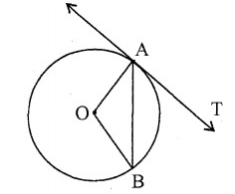
\includegraphics{figs/circfig_1.jpg}
        \caption{}
    \end{figure}    
    \begin{enumerate}
        \item $100^\circ$
        \item $40^\circ$
        \item $50^\circ$
        \item $90^\circ$
    \end{enumerate}\newpage
    \item In figure 3.61, PA and PB are tangents to the circle with centre O. If $\angle APB=100^\circ$, then $\angle OAB$ is
    \begin{figure}[h]
        \centering
        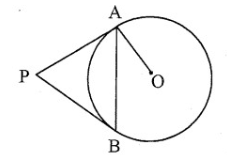
\includegraphics{figs/circfig_2.jpg}
        \caption{}
    \end{figure}
    \begin{enumerate}
        \item $30^\circ$
        \item $60^\circ$
        \item $90^\circ$
        \item $15^\circ$
  \end{enumerate}
    \item The radii of two circles are 4cm and 3cm respectively. The diameter of the circle having area equal to the sum of the area of the two circles (in cm) is
    \begin{enumerate}
        \item 5
        \item 7 
        \item 10
        \item 14
    \end{enumerate}
    \item 	Two concentric circles are of radii $7$ cm and $r$ cm respectively, where $r>7$. A chord of the larger circle, of length $48$ cm, touches the smaller circle. Find the value of $r$.
    \item In figure 3.62, APB and CQD are semi-circles of diameter 7 cm each, while ARC and BSD are semi-circles of diameter 14 cm each. Find the perimeter of the shaded region.[Use $\pi=\dfrac{22}{7}$]
    \begin{figure}[h]
        \centering
        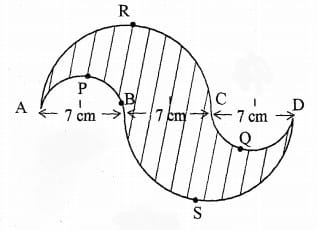
\includegraphics[width=5cm]{figs/circfig_3.jpg}
        \caption{}
    \end{figure}
    \item In figure 3.63, a triangle ABC is drawn to circumscribe a circle of radius 2cm such that the segments BD and DC into which BC is divided by the point of contact D are of lengths 4cm and 3cm respectively. If area of $\triangle ABC=21cm^2$, then find the lengths of sides AB and AC.
    \begin{figure}[h]
        \centering
        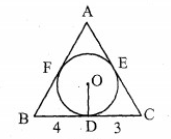
\includegraphics[width=4cm]{figs/circfig_4.jpg}
        \caption{}
    \end{figure}\\
    \item Find the area of the major segment $APB$, in figure 3.64, of a circle of radius $35cm$ and $\angle AOB=90^\circ$.[Use $\pi=\dfrac{22}{7}$]
     \begin{figure}[H]
        \centering
        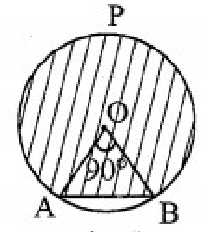
\includegraphics[width=5cm]{figs/circfig_5.jpg}
        \caption{}
    \end{figure}
    
    \item The radii of the circular ends of a bucket of height $15$ $cm$ are $14$ $cm$ and r $cm$ ($r<14$ $cm$). If the volume of bucket is $5390$ $cm^3$, then find the value of $r$.[Use $\pi=\dfrac{22}{7}$]
\end{enumerate}


\chapter{Intersection of Conics}
\section{2022}
\input{2022/chords.tex}
\section{2021}
\subsection{12}
\input{2021/con21.tex}
\section{2019}
\subsection{12}
\input{2019/intersection_19.tex}
\input{2019/inter55.tex}
\section{2018}
\subsection{12}
\input{2018/intersec6.tex}
\input{2018/intco8.tex}





\chapter{Probability}
\section{2021}
\subsection{10}
\input{2021/probability.tex}
\subsection{12}
\input{2021/probability_cbse_21.tex}
\section{2023}
\subsection{10}
\begin{enumerate}
    \item There are two bags $A$ and $B$. Bag $A$ contains $3$ white and $4$ red balls whereas bag $B$ contains $4$ white and $3$ red balls. Three balls are drawn at random (without replacement) from one of the bags and are found to be two white and one red. Find the probability that these were drawn from bag $B$.

    \item Three numbers are selected at random (without replacement) from first six positive integers. If $X$ denotes the smallest of the three numbers obtained, find the probability distribution of $X$. Also find the mean and variance of the distribution.


    \item A bag $X$ contains $4$ white balls and $2$ black balls, while another bag $Y$ contains
          $3$ white balls and $3$ black balls. Two balls are drawn (without replacement) at
          random from one of the bags and were found to be one white and one black.
          Find the probability that the balls were drawn from bag $Y$.

    \item $A$ and $B$ throw a pair of dice alternately, till one of them gets a total of 10 and
          wins the game. Find their respective probabilities of winning, if $A$ starts first.

    \item Three numbers are selected at random (without replacement) from first six
          positive integers. Let $X$ denote the largest of the three numbers obtained. Find
          the probability distribution of $X$. Also, find the mean and variance of the
          distribution.
    \item $A, B$ and $C$ throw a pair of dice in that order alternately till one of them gets a total of $9$ and wins the game. Find their respective probabilities of winning, if $A$ starts first.
    \item A random variable $X$ has the following probability distribution :
          \begin{table}[h!]
              \begin{center}
                  \begin{tabular}{|c |c| c | c | c | c | c | c |}
                      \hline
                      X        & 0   & 1    & 2    & 3    & 4     & 5      & 6         \\
                      \hline
                      $\pr{X}$ & $C$ & $2C$ & $2C$ & $3C$ & $C^2$ & $2C^2$ & $7C^2 +C$ \\
                      \hline
                  \end{tabular}
              \end{center}
          \end{table}
          Find the value of $C$ and also calculate mean of the distribution.
    \item A committee of $4$ students is selected at random from a group consisting of $7$ boys and $4$ girls. Find the probability that there are exactly $2$ boys in the committee, given that at least one girl must be there in the committee.
    \item Five bad oranges are accidently mixed with $20$ good ones. If four oranges are drawn one by one successively with replacement, then find the probability distribution of number of bad oranges drawn. Hence find the mean and variance of the distribution.
    \item In a game, a man wins \rupee $5$ for getting a number greater than $4$ and loses \rupee $1$ otherwise, when a fair die is thrown. The man decided to throw a die thrice but to quit as and when he gets a number greater than $4$. Find the expected value of the amound he wins/loses.
    \item A bag contains $4$ balls. Two balls are drawn at random \brak{\text{without replacement}} and are found to be white. What is the probability that all balls in the bag are white ?
    \item A committee of $4$ students is selected at random from a group consisting of $7$ boys and $4$ girls. Find the probability that there are exactly $2$ boys in the committee, given that at least one girl must be there in the committee.
    \item A random variable $X$ has the following probability distribution:
          \begin{center}
              \begin{tabular}{|c|c|c|c|c|c|c|c|}
                  \hline
                  $X$         & $0$ & $1$  & $2$  & $3$  & $4$   & $5$    & $6$      \\
                  \hline
                  $P\brak{X}$ & $C$ & $2C$ & $2C$ & $3C$ & $C^2$ & $2C^2$ & $7C^2+C$ \\
                  \hline
              \end{tabular}
          \end{center}
          Find the value of $C$ and also calculate mean of the distribution.
    \item $A$, $B$ and $C$ throw a pair of dice in that order alternately till one of them gets a total of $9$ and wins the game. Find their respective probabilities of winning, if $A$ starts first.

    \item A bag $X$ contains $4$ white balls and $2$ black balls, while another bag $Y$ contains $3$ white balls and $3$ black balls. Two balls are drawn (without replacement) at random from one of the bags and were found to be one white and one black. Find the probability that the balls were drawn from bag $Y$.

    \item $A$ and $B$ throw a pair of dice alternately, till one of them gets a total of $10$ and wins the game. Find their respective probabilities of winning, if $A$ starts first.

    \item Three numbers are selected at random (without replacement) from first six positive integers. Let $X$ denote the largest of the three numbers obtained. Find the probability distribution of $X$. Also, find the mean and variance of the distribution.
    \item In a game, a man wins \rupee $5$ for getting a number greater than 4 and loses \rupee $1$ otherwise, then a fair die is thrown. The man decided to throw a die thrice but  quit as and when he gets a number greater than $4$. Find the expected value of the amount he wins/loses.

    \item A bag contains $4$ balls. Two balls are drawn at random (without replacement) and are found to be white. What is the probability that all balls in the bag are white.
    \item A bag $X$ contains $4$ white balls and $2$ black balls, while another bag $Y$ contains $3$ white balls and $3$ black balls. Two balls are drawn (without replacement) at random from  one of the bags and where found to be one white and one black. Find the probability that the balls were  drawn from bag $Y$.
    \item $A$ and $B$ throw a pair of alternatively, till one of them gets a total of $10$ and wins the game. Find their respective probabilities of winning, if $A$ starts first.
    \item Three numbers are selected at random (without replacement) from first six positive integers. Let $X$ denote the largest of the three numbers obtained. Find the probability distribution of $X$. Also, find the mean and variance of the distribution.
    \item A committee of 4 students is selected at random from a group consisting of 7 boys and 4 girls.Find the probability that there are exactly 2 boys in the committee,given that at least one girl must be there in the committee.

    \item A random variable X has the following probability distribution:\\
          \begin{tabular}{|c|c|c|c|c|c|c|c|}
              \hline
              X      & 0   & 1    & 2    & 3    & 4       & 5        & 6          \\
              \hline
              $P(X)$ & $C$ & $2C$ & $2C$ & $3C$ & $C^{2}$ & $2C^{2}$ & $7C^{2}+C$ \\
              \hline
          \end{tabular}\\
          find the value of C and also calculate mean of the distribution.
    \item A,B and C throw a pair of dice in that order alternately till one of them gets a total of 9 and wins the game.Find their respective probabilities of winning if A starts first.
    \item There are two bags A and B.Bag A contains 3 white and 4 red balls whereas bag B contains 4 white and 3 red balls.Three balls are drawn at random(without replacement) from one of the bags are found to be two white and one red.Find the probability that these were drawn from bag B.
    \item There are two bags A and B. Bag A contains $3$ white and $4$ red balls whereas bag B contains $4$ white and $3$ red balls. Three balls are drawn at random (without replacement) from one of the bags and are found to be two white and one red. Find the probability that these were drawn from bag B.
    \item Three numbers are selected at random (without replacement) from first six positive integers. If $X$ denotes the smallest of the three numbers obtained, find the probability distribution of $X$. Also find the mean and variance of the distribution.


\subsection{12}
\input{2023/probability12.tex}
\section{2022}
\subsection{10}
\input{2022/probability10.tex}
\section{2022}
\subsection{12}
\input{2022/probability.tex}
\section{2020}
\subsection{10}
\input{2020/prob10.tex}
\subsection{12}
\input{2020/prob12.tex}
\section{2019}
\subsection{12}
\input{2019/probab_19.tex}
\input{2019/probb55.tex}
\input{2019/prob202.tex}
\input{2019/probab19d.tex}
\input{2019/prob203.tex}
\section{2019}
\subsection{10}
\input{2019/probj.tex}
\section{2018}
\subsection{10}
\input{2018/probability-CBSE.tex}
\input{2018/prob22.tex}
\subsection{12}
\input{2018/probh.tex}
\input{2018/prob6.tex}
\input{2018/pro8.tex}

\section{2017}
\subsection{10}
\input{2017/prob1.tex}
\subsection{12}
\input{2017/prob17.tex}




\section{2016}
\subsection{10}
\input{2016/prob_10.tex}
\subsection{12}
\begin{enumerate}
    \item There are two bags $A$ and $B$. Bag $A$ contains $3$ white and $4$ red balls whereas bag $B$ contains $4$ white and $3$ red balls. Three balls are drawn at random (without replacement) from one of the bags and are found to be two white and one red. Find the probability that these were drawn from bag $B$.

    \item Three numbers are selected at random (without replacement) from first six positive integers. If $X$ denotes the smallest of the three numbers obtained, find the probability distribution of $X$. Also find the mean and variance of the distribution.


    \item A bag $X$ contains $4$ white balls and $2$ black balls, while another bag $Y$ contains
          $3$ white balls and $3$ black balls. Two balls are drawn (without replacement) at
          random from one of the bags and were found to be one white and one black.
          Find the probability that the balls were drawn from bag $Y$.

    \item $A$ and $B$ throw a pair of dice alternately, till one of them gets a total of 10 and
          wins the game. Find their respective probabilities of winning, if $A$ starts first.

    \item Three numbers are selected at random (without replacement) from first six
          positive integers. Let $X$ denote the largest of the three numbers obtained. Find
          the probability distribution of $X$. Also, find the mean and variance of the
          distribution.
    \item $A, B$ and $C$ throw a pair of dice in that order alternately till one of them gets a total of $9$ and wins the game. Find their respective probabilities of winning, if $A$ starts first.
    \item A random variable $X$ has the following probability distribution :
          \begin{table}[h!]
              \begin{center}
                  \begin{tabular}{|c |c| c | c | c | c | c | c |}
                      \hline
                      X        & 0   & 1    & 2    & 3    & 4     & 5      & 6         \\
                      \hline
                      $\pr{X}$ & $C$ & $2C$ & $2C$ & $3C$ & $C^2$ & $2C^2$ & $7C^2 +C$ \\
                      \hline
                  \end{tabular}
              \end{center}
          \end{table}
          Find the value of $C$ and also calculate mean of the distribution.
    \item A committee of $4$ students is selected at random from a group consisting of $7$ boys and $4$ girls. Find the probability that there are exactly $2$ boys in the committee, given that at least one girl must be there in the committee.
    \item Five bad oranges are accidently mixed with $20$ good ones. If four oranges are drawn one by one successively with replacement, then find the probability distribution of number of bad oranges drawn. Hence find the mean and variance of the distribution.
    \item In a game, a man wins \rupee $5$ for getting a number greater than $4$ and loses \rupee $1$ otherwise, when a fair die is thrown. The man decided to throw a die thrice but to quit as and when he gets a number greater than $4$. Find the expected value of the amound he wins/loses.
    \item A bag contains $4$ balls. Two balls are drawn at random \brak{\text{without replacement}} and are found to be white. What is the probability that all balls in the bag are white ?
    \item A committee of $4$ students is selected at random from a group consisting of $7$ boys and $4$ girls. Find the probability that there are exactly $2$ boys in the committee, given that at least one girl must be there in the committee.
    \item A random variable $X$ has the following probability distribution:
          \begin{center}
              \begin{tabular}{|c|c|c|c|c|c|c|c|}
                  \hline
                  $X$         & $0$ & $1$  & $2$  & $3$  & $4$   & $5$    & $6$      \\
                  \hline
                  $P\brak{X}$ & $C$ & $2C$ & $2C$ & $3C$ & $C^2$ & $2C^2$ & $7C^2+C$ \\
                  \hline
              \end{tabular}
          \end{center}
          Find the value of $C$ and also calculate mean of the distribution.
    \item $A$, $B$ and $C$ throw a pair of dice in that order alternately till one of them gets a total of $9$ and wins the game. Find their respective probabilities of winning, if $A$ starts first.

    \item A bag $X$ contains $4$ white balls and $2$ black balls, while another bag $Y$ contains $3$ white balls and $3$ black balls. Two balls are drawn (without replacement) at random from one of the bags and were found to be one white and one black. Find the probability that the balls were drawn from bag $Y$.

    \item $A$ and $B$ throw a pair of dice alternately, till one of them gets a total of $10$ and wins the game. Find their respective probabilities of winning, if $A$ starts first.

    \item Three numbers are selected at random (without replacement) from first six positive integers. Let $X$ denote the largest of the three numbers obtained. Find the probability distribution of $X$. Also, find the mean and variance of the distribution.
    \item In a game, a man wins \rupee $5$ for getting a number greater than 4 and loses \rupee $1$ otherwise, then a fair die is thrown. The man decided to throw a die thrice but  quit as and when he gets a number greater than $4$. Find the expected value of the amount he wins/loses.

    \item A bag contains $4$ balls. Two balls are drawn at random (without replacement) and are found to be white. What is the probability that all balls in the bag are white.
    \item A bag $X$ contains $4$ white balls and $2$ black balls, while another bag $Y$ contains $3$ white balls and $3$ black balls. Two balls are drawn (without replacement) at random from  one of the bags and where found to be one white and one black. Find the probability that the balls were  drawn from bag $Y$.
    \item $A$ and $B$ throw a pair of alternatively, till one of them gets a total of $10$ and wins the game. Find their respective probabilities of winning, if $A$ starts first.
    \item Three numbers are selected at random (without replacement) from first six positive integers. Let $X$ denote the largest of the three numbers obtained. Find the probability distribution of $X$. Also, find the mean and variance of the distribution.
    \item A committee of 4 students is selected at random from a group consisting of 7 boys and 4 girls.Find the probability that there are exactly 2 boys in the committee,given that at least one girl must be there in the committee.

    \item A random variable X has the following probability distribution:\\
          \begin{tabular}{|c|c|c|c|c|c|c|c|}
              \hline
              X      & 0   & 1    & 2    & 3    & 4       & 5        & 6          \\
              \hline
              $P(X)$ & $C$ & $2C$ & $2C$ & $3C$ & $C^{2}$ & $2C^{2}$ & $7C^{2}+C$ \\
              \hline
          \end{tabular}\\
          find the value of C and also calculate mean of the distribution.
    \item A,B and C throw a pair of dice in that order alternately till one of them gets a total of 9 and wins the game.Find their respective probabilities of winning if A starts first.
    \item There are two bags A and B.Bag A contains 3 white and 4 red balls whereas bag B contains 4 white and 3 red balls.Three balls are drawn at random(without replacement) from one of the bags are found to be two white and one red.Find the probability that these were drawn from bag B.
    \item There are two bags A and B. Bag A contains $3$ white and $4$ red balls whereas bag B contains $4$ white and $3$ red balls. Three balls are drawn at random (without replacement) from one of the bags and are found to be two white and one red. Find the probability that these were drawn from bag B.
    \item Three numbers are selected at random (without replacement) from first six positive integers. If $X$ denotes the smallest of the three numbers obtained, find the probability distribution of $X$. Also find the mean and variance of the distribution.


\item There are two bags A and B.Bag A contains 3 white and 4 red balls whereas bag B contains 4 white and 3 red balls.Three balls are drawn at random(without replacement) from one of the bags are found to be two white and one red.Find the probability that these were drawn from bag B.
\item Three numbers are selected at random(without replacement) from first six positive integers.If X denotes the smallest of the three numbers obtained,find the probability distribution of X.Also find the mean and variance of distribution.

\item Three numbers are selected at random (without replacement) from first six positive integers. Let $X$ denote the largest of the three numbers obtained. Find the probability distribution of $X$. Also, find the mean and variance of the distribution.    \item A bag $X$ contains $4$ white balls and $2$ black balls, while another bag $Y$ contains $3$ white balls and $3$ black balls. Two balls are drawn (without replacement) at random from  one of the bags and where found to be one white and one black. Find the probability that the balls were  drawn from bag $Y$.
\item $A$ and $B$ throw a pair of alternatively, till one of them gets a total of $10$ and wins the game. Find their respective probabilities of winning, if $A$ starts first.

\item A committee of 4 students is selected at random from a group consisting of 7 boys and 4 girls.Find the probability that there are exactly 2 boys in the committee,given that at least one girl must be there in the committee.

\item A,B and C throw a pair of dice in that order alternately till one of them gets a total of 9 and wins the game.Find their respective probabilities of winning if A starts first.
 \end{enumerate}

\section{2015}
\subsection{10}
\begin{enumerate}
    \item There are two bags $A$ and $B$. Bag $A$ contains $3$ white and $4$ red balls whereas bag $B$ contains $4$ white and $3$ red balls. Three balls are drawn at random (without replacement) from one of the bags and are found to be two white and one red. Find the probability that these were drawn from bag $B$.

    \item Three numbers are selected at random (without replacement) from first six positive integers. If $X$ denotes the smallest of the three numbers obtained, find the probability distribution of $X$. Also find the mean and variance of the distribution.


    \item A bag $X$ contains $4$ white balls and $2$ black balls, while another bag $Y$ contains
          $3$ white balls and $3$ black balls. Two balls are drawn (without replacement) at
          random from one of the bags and were found to be one white and one black.
          Find the probability that the balls were drawn from bag $Y$.

    \item $A$ and $B$ throw a pair of dice alternately, till one of them gets a total of 10 and
          wins the game. Find their respective probabilities of winning, if $A$ starts first.

    \item Three numbers are selected at random (without replacement) from first six
          positive integers. Let $X$ denote the largest of the three numbers obtained. Find
          the probability distribution of $X$. Also, find the mean and variance of the
          distribution.
    \item $A, B$ and $C$ throw a pair of dice in that order alternately till one of them gets a total of $9$ and wins the game. Find their respective probabilities of winning, if $A$ starts first.
    \item A random variable $X$ has the following probability distribution :
          \begin{table}[h!]
              \begin{center}
                  \begin{tabular}{|c |c| c | c | c | c | c | c |}
                      \hline
                      X        & 0   & 1    & 2    & 3    & 4     & 5      & 6         \\
                      \hline
                      $\pr{X}$ & $C$ & $2C$ & $2C$ & $3C$ & $C^2$ & $2C^2$ & $7C^2 +C$ \\
                      \hline
                  \end{tabular}
              \end{center}
          \end{table}
          Find the value of $C$ and also calculate mean of the distribution.
    \item A committee of $4$ students is selected at random from a group consisting of $7$ boys and $4$ girls. Find the probability that there are exactly $2$ boys in the committee, given that at least one girl must be there in the committee.
    \item Five bad oranges are accidently mixed with $20$ good ones. If four oranges are drawn one by one successively with replacement, then find the probability distribution of number of bad oranges drawn. Hence find the mean and variance of the distribution.
    \item In a game, a man wins \rupee $5$ for getting a number greater than $4$ and loses \rupee $1$ otherwise, when a fair die is thrown. The man decided to throw a die thrice but to quit as and when he gets a number greater than $4$. Find the expected value of the amound he wins/loses.
    \item A bag contains $4$ balls. Two balls are drawn at random \brak{\text{without replacement}} and are found to be white. What is the probability that all balls in the bag are white ?
    \item A committee of $4$ students is selected at random from a group consisting of $7$ boys and $4$ girls. Find the probability that there are exactly $2$ boys in the committee, given that at least one girl must be there in the committee.
    \item A random variable $X$ has the following probability distribution:
          \begin{center}
              \begin{tabular}{|c|c|c|c|c|c|c|c|}
                  \hline
                  $X$         & $0$ & $1$  & $2$  & $3$  & $4$   & $5$    & $6$      \\
                  \hline
                  $P\brak{X}$ & $C$ & $2C$ & $2C$ & $3C$ & $C^2$ & $2C^2$ & $7C^2+C$ \\
                  \hline
              \end{tabular}
          \end{center}
          Find the value of $C$ and also calculate mean of the distribution.
    \item $A$, $B$ and $C$ throw a pair of dice in that order alternately till one of them gets a total of $9$ and wins the game. Find their respective probabilities of winning, if $A$ starts first.

    \item A bag $X$ contains $4$ white balls and $2$ black balls, while another bag $Y$ contains $3$ white balls and $3$ black balls. Two balls are drawn (without replacement) at random from one of the bags and were found to be one white and one black. Find the probability that the balls were drawn from bag $Y$.

    \item $A$ and $B$ throw a pair of dice alternately, till one of them gets a total of $10$ and wins the game. Find their respective probabilities of winning, if $A$ starts first.

    \item Three numbers are selected at random (without replacement) from first six positive integers. Let $X$ denote the largest of the three numbers obtained. Find the probability distribution of $X$. Also, find the mean and variance of the distribution.
    \item In a game, a man wins \rupee $5$ for getting a number greater than 4 and loses \rupee $1$ otherwise, then a fair die is thrown. The man decided to throw a die thrice but  quit as and when he gets a number greater than $4$. Find the expected value of the amount he wins/loses.

    \item A bag contains $4$ balls. Two balls are drawn at random (without replacement) and are found to be white. What is the probability that all balls in the bag are white.
    \item A bag $X$ contains $4$ white balls and $2$ black balls, while another bag $Y$ contains $3$ white balls and $3$ black balls. Two balls are drawn (without replacement) at random from  one of the bags and where found to be one white and one black. Find the probability that the balls were  drawn from bag $Y$.
    \item $A$ and $B$ throw a pair of alternatively, till one of them gets a total of $10$ and wins the game. Find their respective probabilities of winning, if $A$ starts first.
    \item Three numbers are selected at random (without replacement) from first six positive integers. Let $X$ denote the largest of the three numbers obtained. Find the probability distribution of $X$. Also, find the mean and variance of the distribution.
    \item A committee of 4 students is selected at random from a group consisting of 7 boys and 4 girls.Find the probability that there are exactly 2 boys in the committee,given that at least one girl must be there in the committee.

    \item A random variable X has the following probability distribution:\\
          \begin{tabular}{|c|c|c|c|c|c|c|c|}
              \hline
              X      & 0   & 1    & 2    & 3    & 4       & 5        & 6          \\
              \hline
              $P(X)$ & $C$ & $2C$ & $2C$ & $3C$ & $C^{2}$ & $2C^{2}$ & $7C^{2}+C$ \\
              \hline
          \end{tabular}\\
          find the value of C and also calculate mean of the distribution.
    \item A,B and C throw a pair of dice in that order alternately till one of them gets a total of 9 and wins the game.Find their respective probabilities of winning if A starts first.
    \item There are two bags A and B.Bag A contains 3 white and 4 red balls whereas bag B contains 4 white and 3 red balls.Three balls are drawn at random(without replacement) from one of the bags are found to be two white and one red.Find the probability that these were drawn from bag B.
    \item There are two bags A and B. Bag A contains $3$ white and $4$ red balls whereas bag B contains $4$ white and $3$ red balls. Three balls are drawn at random (without replacement) from one of the bags and are found to be two white and one red. Find the probability that these were drawn from bag B.
    \item Three numbers are selected at random (without replacement) from first six positive integers. If $X$ denotes the smallest of the three numbers obtained, find the probability distribution of $X$. Also find the mean and variance of the distribution.


\input{2015/prob5.tex}
\subsection{12}
\input{2015/probab.tex}
\section{2012}
\subsection{10}
\input{2012/probability.tex}

\section{2011}
\subsection{10}

\begin{enumerate}
    \item Which of the following cannot be the probability of an event?
    \begin{enumerate}
        \item 1.5
        \item $\dfrac{3}{5}$
        \item $25\%$
        \item 0.3
    \end{enumerate}
    \item A coin is tossed two times. Find the probability of getting at least one head.
    \item Two dice are rolled once. Find the probability of getting such numbers on two dice, whose product is a perfect square.
    \item A game consists of tossing a coin 3 times and noting its outcome each time. Hanif wins if he gets three heads or three tails, and loses otherwise. Calculate the probability that Hanif will lose the game.



\chapter{Construction}
\section{2023}
\subsection{10}
\input{2023/construction-10th.tex}
\section{2022}
\subsection{10}
\input{2022/construction.tex}
\section{2021}
\subsection{10}
\input{2021/construction.tex}
\section{2020}
\subsection{10}
\input{2020/cont.tex}
\section{2019} 
\subsection{10}
\input{2019/consj.tex}
\section{2018} 
\subsection{10}
\input{2018/construction-CBSE.tex}
\input{2018/con22.tex}
\section{2017}
\subsection{10}
\input{2017/cons1.tex}





\section{2016}
\subsection{10}
\input{2016/construction_10.tex}
\section{2015}
\subsection{10}
\input{2015/construction.tex}
\input{2015/con5.tex}
\section{2012}
\subsection{10}
\input{2012/construction.tex}

\section{2011}
\subsection{10}

\begin{enumerate}
    \item Draw a line segment of length 6 cm. Using compasses and ruler, find a point P on it which divides it in the ratio $3:4$.
    \item Draw a triangle ABC in which AB=5 cm, BC=6 cm and $\angle ABC=60^\circ$. Then construct a triangle whose sides are $\dfrac{5}{7}$ times the corresponding sides of $\triangle ABC$.
\end{enumerate}



\chapter{Optimization}
\section{2023}
\input{2023/opti.tex}
\section{2021}
\subsection{12}
\input{2022/opt_vect.tex}
\section{2022}
\subsection{12}
\input{2021/opti-21-12.tex}
\section{2020}
\subsection{12}
\input{2020/Assignment2.tex}
\section{2019}
\subsection{12}
\input{2019/opti_19.tex}
\input{2019/opt55.tex}
\input{2019/opti202.tex}
\input{2019/opti203.tex}
\section{2018}
\subsection{10}
\input {2018/opt22.tex}
\subsection{12}
\input{2018/opth.tex}
\input{2018/opti6.tex}
\input{2018/opt8.tex}

\section{2017}
\subsection{10}

\subsection{12}
\input{2017/opt17.tex}




\section{2016}
\subsection{12}
\begin{enumerate}
	\item A diet is to contain at least $80$ units of Vitamin $A$ and $100$ units of minerals.
	      Two foods $\text{F}_1$ and $\text{F}_2$ are available costing $5$ rupees per unit and $6$ rupees per unit respectively.
	      One unit of food $\text{F}_1$ contains $4$ units of vitamin $A$ and $3$ units of minerals whereas
	      one unit of food $\text{F}_2$ contains $3$ units of vitamin $A$ and $6$ units of minerals.
	      Formulate this as a linear programming problem. Find the minimum cost of diet that consists of mixture of these two foods and also meets minimum nutritional requirement.


	\item  A retired person wants to invest an amount of $50,000$ rupees. His broker recommends investing in two type of bonds $A$ and $B$ yielding $10\%$ and $9\%$ return respectively on the invested amount. He decides to invest at least
	      $20,000$ rupees in bond $A$ and at least $10,000$ rupees in bond $B$. He also wants to invest at least as much in bond $A$ as in bond $B$. Solve this linear programming problem graphically to maximise his returns.

	\item A typist charges $145$ rupees for typing $10$ English and $3$ Hindi pages, while charges for typing $3$ English and $10$ Hindi pages are $180$ rupees. Using matrices,
	      find the charges of typing one English and one Hindi page separately.
	      However typist charged only $2$ rupees per page from a poor student Shayam for $5$ Hindi pages.
	      How mcuh less was charged from ths poor boy? which values are reflected in this problem?
	\item There are two types of fertilisers $A$ and $B$. $A$ consists of $12$\% nitrogen and $5$\% phosphoric acid whereas $B$ consists of $4$\% nitrogen and $5$\% phosphoric acid. After testing the soil conditions, farmer finds that he needs at least $12$ kg of nitrogen and $12$ kg of phosphoric acid for his crops. If $A$ costs \rupee $10$ per kg and $B$ cost \rupee $8$ per kg, then graphically determine how much of each type of fertiliser should be used so that nutrient requirements are met at a minimum cost.
	\item A company manufactures two types of cardigans : type $A$ and type $B$. It costs \rupee $360$ to make a type $A$ cardigan and \rupee $120$ to make a type $B$ cardigan. The company can make at most $300$ cardigans and spend at most \rupee $72,000$ a day. The number of cardigans of type $B$ cannot exceed the number of cardigans of type $A$ by more than $200$. The company makes a profit of \rupee $100$ for each cardigan of type $A$ and \rupee $50$ for every cardigan of type $B$. Formulate this problem as a linear programming problem to maximise the profit to the company. Solve it graphically and find maximum profit.
	\item A typist charges \rupee $145$ for typing $10$ English and $3$ Hindi pages, while charges for typing $3$ English and $10$ Hindi pages are \rupee $180$. Using matrices, find the charges of typing one English and one English page separately. However typist charged only \rupee $2$ per page from a poor student Shyam for $5$ Hindi pages. How much less was charged from this poor boy? Which values are reflected in this problem?

	\item A retired person wants to invest an amount of \rupee $50,000$. His broker recommends investing in the type of bonds '$A$' and '$B$' yielding $10\%$ and $9\%$ return respectively on the invested amount. He decides to invest at least \rupee $20,000$ in bond '$A$' and at least \rupee $10,000$ in bond '$B$'. He also wants to invest at least as much in bond '$A$' as in bond '$B$'. Solve this linear programming problem graphically to maximise his returns.
	\item There are two types of fertilisers \lq A\rq and \lq B\rq. \lq A\rq consists of $12\%$ nitrogen and $5\%$ phosphoric acid whereas \lq B\rq consists of $4\%$ nitrogen and $5\%$ phosphoric acid. After testing the soil conditions, farmer finds that he needs at least $12$ kg of nitrogen and $12$ kg of phosphoric acid for his crops. If \lq A\rq costs \rupee $10$ per kg and \lq B\rq cost \rupee $8$ per kg, then graphically determine how much of each type of fertiliser should be used so that nutrients requirements are met at a minimum cost.
	\item A company manufactures two types of cardigans:type A and type B.It costs \rupee~360 to make a type A cardigan and \rupee~120 to make a type B cardigan.The company can make at most \rupee~300 cardigans and spend at most \rupee~72000 a day.The number of cardigans of type B cannot exceed the number of cardigans of type A by more than \rupee~200.The company makes a profit of \rupee~100 for each cardigan of type A and \rupee~50 for every cardigan of type B.
	      Formulate this problem as a linear programming problem to maximise the profit to the company.Solve it graphically and find maximum profit.	
 	\item A diet is to contain 80 units of Vitamin A and 100 units of minerals. Two foods $F_1$ and $F_2$ are available, costing \rupee 5 per unit and \rupee 6 per unit, respectively. One unit of food $F_1$ contains 4 units of vitamin A and 3 units of minerals whereas one unit of food $F_2$ contains 3 units of vitamin A and 6 units of minerals. Formulate this as a linear programming problem. Find the minimum cost of diet that consists of mixture of these two foods and also meets minimum nutritional requirement.




\item A diet is to contain at least 80 units of vitamin A and 100 units of minerals.Two foods F1 and F2 are available at costing \rupee~5 per unit \rupee~6 per unit respectively.One unit of food F1 contains 4 units of vitamin A and 3 units of minerals whereas one unit of food F2 contains  3 units of vitamins A and 6 units of minerals.Formulate this as a linear programming problem.Find the minimum cost of diet that consists of mixture of these two foods and also meets minimum nutritional requirement.
 
     \item A company manufactures two types of cardigans:type A and type B.It costs \rupee~360 to make a type A cardigan and \rupee~120 to make a type B cardigan.The company can make at most \rupee~300 cardigans and spend at most \rupee~72000 a day.The number of cardigans of type B cannot exceed the number of cardigans of type A by more than \rupee~200.The company makes a profit of \rupee~100 for each cardigan of type A and \rupee~50 for every cardigan of type B.
 Formulate this problem as a linear programming problem to maximise the profit to the company.Solve it graphically and find maximum profit.

 \end{enumerate}



\section{2015}
\subsection{12}
\begin{enumerate}
	\item A diet is to contain at least $80$ units of Vitamin $A$ and $100$ units of minerals.
	      Two foods $\text{F}_1$ and $\text{F}_2$ are available costing $5$ rupees per unit and $6$ rupees per unit respectively.
	      One unit of food $\text{F}_1$ contains $4$ units of vitamin $A$ and $3$ units of minerals whereas
	      one unit of food $\text{F}_2$ contains $3$ units of vitamin $A$ and $6$ units of minerals.
	      Formulate this as a linear programming problem. Find the minimum cost of diet that consists of mixture of these two foods and also meets minimum nutritional requirement.


	\item  A retired person wants to invest an amount of $50,000$ rupees. His broker recommends investing in two type of bonds $A$ and $B$ yielding $10\%$ and $9\%$ return respectively on the invested amount. He decides to invest at least
	      $20,000$ rupees in bond $A$ and at least $10,000$ rupees in bond $B$. He also wants to invest at least as much in bond $A$ as in bond $B$. Solve this linear programming problem graphically to maximise his returns.

	\item A typist charges $145$ rupees for typing $10$ English and $3$ Hindi pages, while charges for typing $3$ English and $10$ Hindi pages are $180$ rupees. Using matrices,
	      find the charges of typing one English and one Hindi page separately.
	      However typist charged only $2$ rupees per page from a poor student Shayam for $5$ Hindi pages.
	      How mcuh less was charged from ths poor boy? which values are reflected in this problem?
	\item There are two types of fertilisers $A$ and $B$. $A$ consists of $12$\% nitrogen and $5$\% phosphoric acid whereas $B$ consists of $4$\% nitrogen and $5$\% phosphoric acid. After testing the soil conditions, farmer finds that he needs at least $12$ kg of nitrogen and $12$ kg of phosphoric acid for his crops. If $A$ costs \rupee $10$ per kg and $B$ cost \rupee $8$ per kg, then graphically determine how much of each type of fertiliser should be used so that nutrient requirements are met at a minimum cost.
	\item A company manufactures two types of cardigans : type $A$ and type $B$. It costs \rupee $360$ to make a type $A$ cardigan and \rupee $120$ to make a type $B$ cardigan. The company can make at most $300$ cardigans and spend at most \rupee $72,000$ a day. The number of cardigans of type $B$ cannot exceed the number of cardigans of type $A$ by more than $200$. The company makes a profit of \rupee $100$ for each cardigan of type $A$ and \rupee $50$ for every cardigan of type $B$. Formulate this problem as a linear programming problem to maximise the profit to the company. Solve it graphically and find maximum profit.
	\item A typist charges \rupee $145$ for typing $10$ English and $3$ Hindi pages, while charges for typing $3$ English and $10$ Hindi pages are \rupee $180$. Using matrices, find the charges of typing one English and one English page separately. However typist charged only \rupee $2$ per page from a poor student Shyam for $5$ Hindi pages. How much less was charged from this poor boy? Which values are reflected in this problem?

	\item A retired person wants to invest an amount of \rupee $50,000$. His broker recommends investing in the type of bonds '$A$' and '$B$' yielding $10\%$ and $9\%$ return respectively on the invested amount. He decides to invest at least \rupee $20,000$ in bond '$A$' and at least \rupee $10,000$ in bond '$B$'. He also wants to invest at least as much in bond '$A$' as in bond '$B$'. Solve this linear programming problem graphically to maximise his returns.
	\item There are two types of fertilisers \lq A\rq and \lq B\rq. \lq A\rq consists of $12\%$ nitrogen and $5\%$ phosphoric acid whereas \lq B\rq consists of $4\%$ nitrogen and $5\%$ phosphoric acid. After testing the soil conditions, farmer finds that he needs at least $12$ kg of nitrogen and $12$ kg of phosphoric acid for his crops. If \lq A\rq costs \rupee $10$ per kg and \lq B\rq cost \rupee $8$ per kg, then graphically determine how much of each type of fertiliser should be used so that nutrients requirements are met at a minimum cost.
	\item A company manufactures two types of cardigans:type A and type B.It costs \rupee~360 to make a type A cardigan and \rupee~120 to make a type B cardigan.The company can make at most \rupee~300 cardigans and spend at most \rupee~72000 a day.The number of cardigans of type B cannot exceed the number of cardigans of type A by more than \rupee~200.The company makes a profit of \rupee~100 for each cardigan of type A and \rupee~50 for every cardigan of type B.
	      Formulate this problem as a linear programming problem to maximise the profit to the company.Solve it graphically and find maximum profit.	
 	\item A diet is to contain 80 units of Vitamin A and 100 units of minerals. Two foods $F_1$ and $F_2$ are available, costing \rupee 5 per unit and \rupee 6 per unit, respectively. One unit of food $F_1$ contains 4 units of vitamin A and 3 units of minerals whereas one unit of food $F_2$ contains 3 units of vitamin A and 6 units of minerals. Formulate this as a linear programming problem. Find the minimum cost of diet that consists of mixture of these two foods and also meets minimum nutritional requirement.





\chapter{Algebra}
\section{2020}
\subsection{10}
\input{2020/ALGEBRA-CBSE-10.tex}
\section{2020}
\subsection{12}
\input{2020/ALGEBRA-CBSE-12.tex}
\section{2023}
\subsection{10}
\begin{enumerate}
	\item Prove that $ 2\sin^{-1} \brak{\frac{3}{5}} - \tan^{-1} \brak{\frac{17}{31}} = \frac{\pi}{4}$

	\item Solve the equation for $x$: $\cos (\tan^{-1}) = \sin \brak{\cot^{-1} \frac{3}{4}} = \sin \brak{\cot^{-1} \frac{3}{4}}$

	
	\item Solve for 
	\begin{align*}
		x: \tan^{-1}(x-1) + \tan^{-1}x + \tan^{-1}(x+1) = \tan^{-1}3x
	\end{align*}

	\item Prove that 
	\begin{align*}
	\tan^{-1} \brak{\frac{6x-8x^{3}}{1-12x^{2}}} - \tan^{-1} \brak{\frac{4x}{1-4x^{2}}} = \tan^{-1}2x;
	\end{align*}
	\begin{align*}
		\abs{2x} < \frac{1}{\sqrt{3}}
	\end{align*}

	\item The equation of tangent at $\brak{2,3}$ on the curve $y^2 = ax^3 + b$ is $4x -5$. Find the values of $a$ and $b$.
	\item Prove that the curves $y^2 = 4x$ and $x^2 = 4y$ divide the area of square bounded by $x=0, x=4, y=4$ and $y=0$ into three equal parts.
	\item Find the equation of the tangent line to the curve $y = \sqrt{5x - 3} - 5$, which is parallel to the line $4x - 2y + 5 = 0$.
 	\item Prove that 
	\begin{align*}
		2\sin^{-1}\brak{\frac{3}{5}}-\tan^{-1}\brak{\frac{17}{31}} = \frac{\pi}{4}
	\end{align*}
	\item Solve the equation for x:
	\begin{align*}
	\cos\brak{\tan^{-1}x} = \sin\brak{\cot^{-1}\frac{3}{4}}
	\end{align*}


\section{2022}
\subsection{10}
\begin{enumerate}
	\item Prove that $ 2\sin^{-1} \brak{\frac{3}{5}} - \tan^{-1} \brak{\frac{17}{31}} = \frac{\pi}{4}$

	\item Solve the equation for $x$: $\cos (\tan^{-1}) = \sin \brak{\cot^{-1} \frac{3}{4}} = \sin \brak{\cot^{-1} \frac{3}{4}}$

	
	\item Solve for 
	\begin{align*}
		x: \tan^{-1}(x-1) + \tan^{-1}x + \tan^{-1}(x+1) = \tan^{-1}3x
	\end{align*}

	\item Prove that 
	\begin{align*}
	\tan^{-1} \brak{\frac{6x-8x^{3}}{1-12x^{2}}} - \tan^{-1} \brak{\frac{4x}{1-4x^{2}}} = \tan^{-1}2x;
	\end{align*}
	\begin{align*}
		\abs{2x} < \frac{1}{\sqrt{3}}
	\end{align*}

	\item The equation of tangent at $\brak{2,3}$ on the curve $y^2 = ax^3 + b$ is $4x -5$. Find the values of $a$ and $b$.
	\item Prove that the curves $y^2 = 4x$ and $x^2 = 4y$ divide the area of square bounded by $x=0, x=4, y=4$ and $y=0$ into three equal parts.
	\item Find the equation of the tangent line to the curve $y = \sqrt{5x - 3} - 5$, which is parallel to the line $4x - 2y + 5 = 0$.
 	\item Prove that 
	\begin{align*}
		2\sin^{-1}\brak{\frac{3}{5}}-\tan^{-1}\brak{\frac{17}{31}} = \frac{\pi}{4}
	\end{align*}
	\item Solve the equation for x:
	\begin{align*}
	\cos\brak{\tan^{-1}x} = \sin\brak{\cot^{-1}\frac{3}{4}}
	\end{align*}


\section{2021}
\subsection{10}
\begin{enumerate}
	\item Prove that $ 2\sin^{-1} \brak{\frac{3}{5}} - \tan^{-1} \brak{\frac{17}{31}} = \frac{\pi}{4}$

	\item Solve the equation for $x$: $\cos (\tan^{-1}) = \sin \brak{\cot^{-1} \frac{3}{4}} = \sin \brak{\cot^{-1} \frac{3}{4}}$

	
	\item Solve for 
	\begin{align*}
		x: \tan^{-1}(x-1) + \tan^{-1}x + \tan^{-1}(x+1) = \tan^{-1}3x
	\end{align*}

	\item Prove that 
	\begin{align*}
	\tan^{-1} \brak{\frac{6x-8x^{3}}{1-12x^{2}}} - \tan^{-1} \brak{\frac{4x}{1-4x^{2}}} = \tan^{-1}2x;
	\end{align*}
	\begin{align*}
		\abs{2x} < \frac{1}{\sqrt{3}}
	\end{align*}

	\item The equation of tangent at $\brak{2,3}$ on the curve $y^2 = ax^3 + b$ is $4x -5$. Find the values of $a$ and $b$.
	\item Prove that the curves $y^2 = 4x$ and $x^2 = 4y$ divide the area of square bounded by $x=0, x=4, y=4$ and $y=0$ into three equal parts.
	\item Find the equation of the tangent line to the curve $y = \sqrt{5x - 3} - 5$, which is parallel to the line $4x - 2y + 5 = 0$.
 	\item Prove that 
	\begin{align*}
		2\sin^{-1}\brak{\frac{3}{5}}-\tan^{-1}\brak{\frac{17}{31}} = \frac{\pi}{4}
	\end{align*}
	\item Solve the equation for x:
	\begin{align*}
	\cos\brak{\tan^{-1}x} = \sin\brak{\cot^{-1}\frac{3}{4}}
	\end{align*}


\input{2021/algebra2021.tex}

\section{2021}
\subsection{12}
\input{2021/Algebra12.tex}

\section{2019}
\subsection{12}
\input{2019/algeb_19.tex}
\input{2019/alger55.tex}
\input{2019/Alg203.tex}
\section{2019} 
\subsection{10}
\input{2019/algebj.tex}
\section{2018} 
\subsection{10}
\input{2018/Algebra-CBSE.tex}
\input{2018/alg22.tex}
\subsection{12}
\input{2018/algh.tex}
\input{2018/alge6.tex}
\input{2018/al8.tex}

\section{2017}
\subsection{10}
\input{2017/alge1.tex}
\subsection{12}
\input{2017/alg17.tex}



\section{2016}
\subsection{10}
\input{2016/alg_10.tex}
\subsection{12}
\begin{enumerate}
	\item Prove that $ 2\sin^{-1} \brak{\frac{3}{5}} - \tan^{-1} \brak{\frac{17}{31}} = \frac{\pi}{4}$

	\item Solve the equation for $x$: $\cos (\tan^{-1}) = \sin \brak{\cot^{-1} \frac{3}{4}} = \sin \brak{\cot^{-1} \frac{3}{4}}$

	
	\item Solve for 
	\begin{align*}
		x: \tan^{-1}(x-1) + \tan^{-1}x + \tan^{-1}(x+1) = \tan^{-1}3x
	\end{align*}

	\item Prove that 
	\begin{align*}
	\tan^{-1} \brak{\frac{6x-8x^{3}}{1-12x^{2}}} - \tan^{-1} \brak{\frac{4x}{1-4x^{2}}} = \tan^{-1}2x;
	\end{align*}
	\begin{align*}
		\abs{2x} < \frac{1}{\sqrt{3}}
	\end{align*}

	\item The equation of tangent at $\brak{2,3}$ on the curve $y^2 = ax^3 + b$ is $4x -5$. Find the values of $a$ and $b$.
	\item Prove that the curves $y^2 = 4x$ and $x^2 = 4y$ divide the area of square bounded by $x=0, x=4, y=4$ and $y=0$ into three equal parts.
	\item Find the equation of the tangent line to the curve $y = \sqrt{5x - 3} - 5$, which is parallel to the line $4x - 2y + 5 = 0$.
 	\item Prove that 
	\begin{align*}
		2\sin^{-1}\brak{\frac{3}{5}}-\tan^{-1}\brak{\frac{17}{31}} = \frac{\pi}{4}
	\end{align*}
	\item Solve the equation for x:
	\begin{align*}
	\cos\brak{\tan^{-1}x} = \sin\brak{\cot^{-1}\frac{3}{4}}
	\end{align*}


\item Ishan wants to donate a rectangular plot of land for a school in his village .When he was asked to give dimensions of the plot,he told that if its length is decreased by 50m and breadth is increased by 50m,then its area will remain same,but if its length is decreased by 10m and breadth is decreased by 20m,then its area will decrease by 5300 $m^{2}$. Using matrices,find the dimensions of plot.Also give reason why he wants to donate the plot for a school.
\item A diet is to contain at least 80 units of vitamin A and 100 units of minerals.Two foods F1 and F2 are available at costing \rupee~5 per unit \rupee~6 per unit respectively.One unit of food F1 contains 4 units of vitamin A and 3 units of minerals whereas one unit of food F2 contains  3 units of vitamins A and 6 units of minerals.Formulate this as a linear programming problem.Find the minimum cost of diet that consists of mixture of these two foods and also meets minimum nutritional requirement.
\item A company manufactures two types of cardigans:type A and type B.It costs \rupee~360 to make a type A cardigan and \rupee~120 to make a type B cardigan.The company can make at most \rupee~300 cardigans and spend at most \rupee~72000 a day.The number of cardigans of type B cannot exceed the number of cardigans of type A by more than \rupee~200.The company makes a profit of \rupee~100 for each cardigan of type A and \rupee~50 for every cardigan of type B. Formulate this problem as a linear programming problem to maximise the profit to the company.Solve it graphically and find maximum profit.
\item A retired person wants to invest an amount  of \rupee~50,000. His broker recommends investing in two type of bonds $'A'$ and $'B'$ yielding $10\%$ and $9\%$ return respectively on the invested amount. He decides to invest at least \rupee~20,000 in bond $'A'$ and at least \rupee~10,000 in bond $'B'$. He also wants to invest at least as much in bond $'A'$ as in bond $'B'$. Solve this linear programming problem graphically to maximise his returns.
\item Write the coordinates of the point which is the reflection of the point$({\alpha},{\beta},{\gamma}) $ in the $ XZ$ - plane.
																				      								        																																					\item On her birthday Seema decided to donate some money to children of an orphanage home. If there were 8 children less,every one would have got \rupee~10 more.However,if there were 16 children more,every one would have got \rupee~10 less.Using matrix method,find the number of children and the amount distributed by Seema.What values are reflected by Seema's decision?
\item Find the coordinates of the foot of perpendicular and perpendicular distance from the point p(4,3,2) to the plane x+2y+3z=2.Also find the image of P in the plane.
\item A typist charges \rupee~145 for typing $10$ English and $3$ Hindi pages, while charges for typing $3$ English and $10$ Hindi pages are \rupee~180. Using matrices, find the charges of typing one English and one Hindi page separately. However typist charged only \rupee~2 per page from poor student Shyam for $5$ Hindi pages. How much less was charged from this poor boy? Which values are reflected in this problem.
\item For what values of $k$, the system of linear equations\\
$x+y+z=2$\\
$2x+y-z=3$\\
$3x+2y+kz=4$\\
has a unique solution?								   
																																																									 
\end{enumerate}
	

\section{2015}
\subsection{10}
\begin{enumerate}
	\item Prove that $ 2\sin^{-1} \brak{\frac{3}{5}} - \tan^{-1} \brak{\frac{17}{31}} = \frac{\pi}{4}$

	\item Solve the equation for $x$: $\cos (\tan^{-1}) = \sin \brak{\cot^{-1} \frac{3}{4}} = \sin \brak{\cot^{-1} \frac{3}{4}}$

	
	\item Solve for 
	\begin{align*}
		x: \tan^{-1}(x-1) + \tan^{-1}x + \tan^{-1}(x+1) = \tan^{-1}3x
	\end{align*}

	\item Prove that 
	\begin{align*}
	\tan^{-1} \brak{\frac{6x-8x^{3}}{1-12x^{2}}} - \tan^{-1} \brak{\frac{4x}{1-4x^{2}}} = \tan^{-1}2x;
	\end{align*}
	\begin{align*}
		\abs{2x} < \frac{1}{\sqrt{3}}
	\end{align*}

	\item The equation of tangent at $\brak{2,3}$ on the curve $y^2 = ax^3 + b$ is $4x -5$. Find the values of $a$ and $b$.
	\item Prove that the curves $y^2 = 4x$ and $x^2 = 4y$ divide the area of square bounded by $x=0, x=4, y=4$ and $y=0$ into three equal parts.
	\item Find the equation of the tangent line to the curve $y = \sqrt{5x - 3} - 5$, which is parallel to the line $4x - 2y + 5 = 0$.
 	\item Prove that 
	\begin{align*}
		2\sin^{-1}\brak{\frac{3}{5}}-\tan^{-1}\brak{\frac{17}{31}} = \frac{\pi}{4}
	\end{align*}
	\item Solve the equation for x:
	\begin{align*}
	\cos\brak{\tan^{-1}x} = \sin\brak{\cot^{-1}\frac{3}{4}}
	\end{align*}


\input{2015/alg5.tex}
\subsection{12}
\input{2015/alg.tex}
\section{2012}
\subsection{10}
\begin{enumerate}
\item The roots of the quadratic equation  $2x^2 - x - 6 = 0$ are 
\begin{enumerate}
\item $-2,\dfrac{3}{2}$ 
\item $2,-\dfrac{3}{2}$ 
\item $-2,-\dfrac{3}{2}$ 
\item $2,\dfrac{3}{2}$ 
\end{enumerate}
\item If $1$ is a root of the equations $ay^2 + ay + 3 = 0$ and $y^2 + y + b = 0$, then $ab$ equals : 
\begin{enumerate}
\item $3$ 
\item $-\dfrac{7}{2}$ 
\item $6$ 
\item $-3$ 
\end{enumerate}
\item If the quadratic equation $mx^2 + 2x + m = 0$ has two equal roots, then the values of $m$ are : 
\begin{enumerate}
\item $\pm 1$ 
\item $0,2$ 
\item $0,1$ 
\item $-1,0$ 
\end{enumerate}
%algebra
\item Find the value of $p$ for which the roots of the equation $px\brak{x-2} + 6 = 0$, are equal. 
%Algebra
\item Solve the following quadratic equation for $x$ : 
\begin{align}
x^2 - 4 a x - b^2 + 4a^2 = 0 
\end{align}
%algebra
%algebra
\item Find the value$\brak{\text{s}}$ of $k$ so that the quadratic equation $x^2 - 4kx + k = 0$ has equal roots. 
%algebra
\item Solve for $x$: $4x^2 - 4ax + \brak{a^2 - b^2} = 0$ 
%algebra
\item Solve for $x$: $3x^2 - 2\sqrt 6 x + 2 = 0$ 

\item Find the value of $k$ for which the roots of the quadratic equation $\brak{k - 4} x^2 + 2\brak{k-4} x + 2 =0$ are equal. 
\item Solve for x: 
$4\sqrt 3 x^2 + 5x - 2\sqrt 3 = 0$ 
\end{enumerate}


\section{2011}
\subsection{10}
\begin{enumerate}
    \item The roots of the equation constant, are $x^2+x-p\brak{p+1}=0$, where p is a constant,are
        \begin{enumerate}
            \item $p,\brak{p+1}$
            \item $-p,\brak{p+1}$
            \item $p,-\brak{p+1}$
            \item $-p,-\brak{p+1}$
        \end{enumerate}
    \item Find the value of $p$ so that the quadratic equation $px\brak{x-3}+9=0$ has two equal roots.
    \item Find the roots of the following quadratic equation:\[2\sqrt{3}x^2-5x+\sqrt{3}=0\]
    \item A motor boat whose speed is $20$$km/h$ in still water, takes 1 hour more to go 48 km upstream than to return downstream to the same spot. Find the speed of the stream.    
    \item Find the roots of the equation \[\dfrac{1}{x+4}-\dfrac{1}{x-7}=\dfrac{11}{30}, x\neq -4,7\] 
\end{enumerate}



\chapter{Geometry}
\section{2023}
\subsection{10}
\input{2023/ASSIGNMENT_1.tex}
\input{2023/latexwork.tex}
\section{2022}
\subsection{10}
\input{2022/latex.tex}

\section{2021}
\subsection{10}
\input{2021/geometry2021.tex}
\section{2020}
\subsection{10}
\input{2020/Gupdates_10.tex}
\section{2019}
\subsection{10}
\input{2019/geoj.tex}
\section{2018}
\subsection{10}
\input{2018/Geometry-CBSE.tex}
\input{2018/geo22.tex}
\subsection{12}
\input{2018/geoh.tex}
\input{2018/geo6.tex}

\section{2017}
\subsection{10}
\input{2017/geo1.tex}
\subsection{12}
\input{2017/geom17.tex}



\section{2016}
\subsection{10}
\input{2016/geometry_10.tex}
\subsection{12}
\begin{enumerate}
    \item Show that the lines
          \begin{align*}
              \dfrac{x-1}{3} & = \dfrac{y-1}{-1} = \dfrac{z+1}{0} \\
              \dfrac{x-4}{2} & = \dfrac{y}{0} = \dfrac{z+1}{3}
          \end{align*}
          intersect. Find their point of intersection.
    \item Find the equation of the tangent line to the curve $y=\sqrt{5x-3} -5$, which is parallel to line
          \begin{align*}
              4x-2y+5=0
          \end{align*}
    \item Write the coordinates fo the point which is the reflection of the point \brak{\alpha,\beta,\gamma} in the $XZ$-plane.
    \item The equation of tangent at \brak{2,3} on the curve
          \begin{align*}
              y^2 & = ax^3 + b \text { is} \\
              y   & = 4x -5
          \end{align*}
          Find the values of $a$ and $b$
    \item Prove that the least perimeter of an isosceles triangle in which a circle of radius $r$ can be inscribed is $6 \sqrt{3} r$
    \item If the sum of lengths of hypotenuse and a side of a right angled triangle is given, show that area of triangle is maximum, when the angle between them is $\dfrac{\pi}{3}$.
    \item Prove that the curves $y^2=4x$ and $x^2= 4y$ divide the area of square bounded by $x=0,y=4$ and $y=0$ into three equal parts.
    \item Show that height of the cylinder of greatest volume which can be inscribed in a right circular cone of height $h$ and semi-vertical angle $\alpha$ is one third that of the cone and the greatest volume of the cyclinder is $\dfrac{4}{27}\pi h^3\tan^2\alpha$.
    \item Find the coordinates of the foot of perpendicular drawn from the point $A\brak{-1,8,4}$ to the line joining the points $B\brak{0,-1,3}$ and $A\brak{2,3,-1}$. Hence find the image of the point $A$ in the line $BC$.

    \item Show that the four point $A\brak{4, 5, 1}, B\brak{0,-1,-1}, C\brak{3,9,4} \text{ and } D\brak{-4,4,4}$ are coplanar.
    \item Find the equation of the tangent line to the curve $y = \sqrt{5x-3} -5$, which is parallel to the line
              {4x-2y+5=0.}
    \item Show that the lines $\frac{x-1}{3} = \frac{y-1}{-1} = \frac{z+1}{0} $ and $\frac{x-4}{2} = \frac{y}{0} = \frac{z+1}{3} $ intersect.Find their point of intersection.
    \item Find the coordinates of the foot of perpendicular and perpendicular distance from the point p(4,3,2) to the plane x+2y+3z=2.Also find the image of P in the plane.




\item Write the coordinates of the point which is the reflection of the point$({\alpha},{\beta},{\gamma}) $ in the $ XZ$ - plane.
\item On her birthday Seema decided to donate some money to children of an orphanage home. If there were 8 children less,every one would have got \rupee~10 more.However,if there were 16 children more,every one would have got \rupee~10 less.Using matrix method,find the number of children and the amount distributed by Seema.What values are reflected by Seema's decision?
\item Find the coordinates of the foot of perpendicular and perpendicular distance from the point p(4,3,2) to the plane x+2y+3z=2.Also find the image of P in the plane.
 \item Show that height of the cylinder of greatest volume which can be inscribed in a right circular cone of height $h$ and semi-vertical angle $\alpha$ is one-third that of the cone and the greatest volume of the cylinder is $\frac{4}{27}\pi h^{3}\tan^{2}\alpha$
\end{enumerate}									

\section{2015}
\subsection{10}
\input{2015/geometry.tex}
\input{2015/geo5.tex}
\section{2012}
\subsection{10}
\input{2012/geometry.tex}
%\input{2023/gouthami.tex}
%\input{2023/algebra-10.tex}
%\subsection{10}
%\input{2023/bindhu.tex}
\section{2011}
\subsection{10}
\begin{enumerate}
    \item A sphere of diameter 18 cm is dropped into a cylindrical vessel of diameter 36 cm, partly filled with water. If the sphere is completely submerged, then the water level rises (in cm) by
    \begin{enumerate}
        \item 3
        \item 4 
        \item 5
        \item 6
    \end{enumerate}
    \item Two cubes, each of side 4 cm are joined end to end. Find the surface area of the resulting cuboid.
    \item Find that value(s) of x for which the distance between the points $P(x,4)$ and $Q(9,10)$ is $10$units.
    \item From a solid cylinder whose height is 15 cm and diameter 16 cm, a conical cavity of the same height and same diameter is hollowed out. Find the total surface area of the remaining solid. [Take $n=3.14$]
\end{enumerate}


\chapter{Discrete}
\section{2022}
\subsection{10}
\input{2022/discrete.tex}
\section{2023}
\subsection{10}
\input{2023/firstlatex.tex}
\section{2021}
\subsection{10}
\input{2021/discrete_21.tex}
\section{2020}
\subsection{10}
\input{2020/dist.tex}
\section{2019}
\subsection{10}
\input{2019/dissj.tex}
\section{2018}
\subsection{10}
\input{2018/discrete-CBSE.tex}
\subsection{12}
\input{2018/dish.tex}
\section{2017}
\subsection{10}
\input{2017/dis1.tex}



\section{2016}
\subsection{10}
\input{2016/discrete_10.tex}
\section{2015}
\subsection{10}
\input{2015/dis5.tex}

%\subsection{12}
%\begin{enumerate}
    \item Show that the lines
          \begin{align*}
              \dfrac{x-1}{3} & = \dfrac{y-1}{-1} = \dfrac{z+1}{0} \\
              \dfrac{x-4}{2} & = \dfrac{y}{0} = \dfrac{z+1}{3}
          \end{align*}
          intersect. Find their point of intersection.
    \item Find the equation of the tangent line to the curve $y=\sqrt{5x-3} -5$, which is parallel to line
          \begin{align*}
              4x-2y+5=0
          \end{align*}
    \item Write the coordinates fo the point which is the reflection of the point \brak{\alpha,\beta,\gamma} in the $XZ$-plane.
    \item The equation of tangent at \brak{2,3} on the curve
          \begin{align*}
              y^2 & = ax^3 + b \text { is} \\
              y   & = 4x -5
          \end{align*}
          Find the values of $a$ and $b$
    \item Prove that the least perimeter of an isosceles triangle in which a circle of radius $r$ can be inscribed is $6 \sqrt{3} r$
    \item If the sum of lengths of hypotenuse and a side of a right angled triangle is given, show that area of triangle is maximum, when the angle between them is $\dfrac{\pi}{3}$.
    \item Prove that the curves $y^2=4x$ and $x^2= 4y$ divide the area of square bounded by $x=0,y=4$ and $y=0$ into three equal parts.
    \item Show that height of the cylinder of greatest volume which can be inscribed in a right circular cone of height $h$ and semi-vertical angle $\alpha$ is one third that of the cone and the greatest volume of the cyclinder is $\dfrac{4}{27}\pi h^3\tan^2\alpha$.
    \item Find the coordinates of the foot of perpendicular drawn from the point $A\brak{-1,8,4}$ to the line joining the points $B\brak{0,-1,3}$ and $A\brak{2,3,-1}$. Hence find the image of the point $A$ in the line $BC$.

    \item Show that the four point $A\brak{4, 5, 1}, B\brak{0,-1,-1}, C\brak{3,9,4} \text{ and } D\brak{-4,4,4}$ are coplanar.
    \item Find the equation of the tangent line to the curve $y = \sqrt{5x-3} -5$, which is parallel to the line
              {4x-2y+5=0.}
    \item Show that the lines $\frac{x-1}{3} = \frac{y-1}{-1} = \frac{z+1}{0} $ and $\frac{x-4}{2} = \frac{y}{0} = \frac{z+1}{3} $ intersect.Find their point of intersection.
    \item Find the coordinates of the foot of perpendicular and perpendicular distance from the point p(4,3,2) to the plane x+2y+3z=2.Also find the image of P in the plane.



\section{2012}
\subsection{10}
\input{2012/discrete.tex}
\section{2011}
\subsection{10}
\begin{enumerate}
    \item In an AP, if d=2, n=5 and $a_n=0$, then value of a is
    \begin{enumerate}
        \item 10
        \item 5
        \item -8
        \item 8
    \end{enumerate}
    \item Find whether -150 is a term of the AP 17, 12, 7, 2,....?
    \item Find the value of the middle term of the following AP :\[- 6, -2, 2,........, 58.\]
   \item Determine the AP whose fourth term is 18 and the difference of the ninth term from the fifteenth term is 30.
\end{enumerate}


\chapter{Number Systems}
\section{2019}
\subsection{10}
\input{2019/numsysj.tex}
\section{2018}
\subsection{10}
\input{2018/num22.tex}
\section{2012}
\subsection{10}
\input{2012/number_sys.tex}


\chapter{Differentiation}
\section{2023}
\subsection{12}
\input{2023/differentiation.tex}

\section{2022}
\subsection{12}
\input{2022/maths.tex}
\section{2021}
\subsection{10}
\begin{enumerate}
    \item Differentiate $(\sin 2x)^x + \sin^{-1} \sqrt{3x}$ with respect to $x$.

    \item Differentiate $\tan^{-1} \brak{\frac{\sqrt{1 + x^2}-\sqrt{1-x^2}}{\sqrt{1+x^2}+\sqrt{1-x^2}}}$
          with respect to $\cos^{-1} x^2$.

    \item Determine the intervals in which the function $f (x) = x^4 - 8x^3 + 22x^2 - 24x+21$ is strictly increasing or strictly decreasing.

    \item Find the maximum and minimum values of $f (x) = \sec x + \log \cos^2 x$, $0 < x < 2\pi$.

    \item Find the eqaution of normal to the curve $ay^2 = x^3$ at the point whose $x$ coordinate is $am^2$


    \item If $\cos(a+y) = \cos y$ then prove that
          $\dfrac{dy}{dx} = \frac{\cos^{2}(a+y)}{\sin a}$.
          Hence show that \\
          $\sin a \dfrac{d^{2}y}{dx^{2}} + \sin 2(a+y)\dfrac{dy}{dx} = 0 $.

    \item Find $\dfrac{dy}{dx}$ if $y = \sin^{-1}\sbrak{\frac{6x - 4\sqrt{1-4x^2}}{5}}$

    \item Find the equation of the tangents to the curve $y = x^3 + 2x - 4$ which are perpendicular to line $x + 14y + 3 = 0$

    \item Show that semi-vertical angle of a cone of maximum volume and given slant height is
          $\cos^{-1}\brak{ \frac{1}{\sqrt{3}}}$

    \item Prove that $ y = \frac{4\sin \theta}{2+ \cos \theta} - \theta$ ia an increasing function of $\theta$ on $\sbrak{0,\frac{\pi}{2}}$.
    \item If $x=e^{\cos 2t}$ and $y=e^{\sin 2t}$, prove that
          \begin{align*}
              \dfrac{dy}{dx}= -\dfrac{y \log x}{x \log y}
          \end{align*}
    \item Differentiate $x^{\sin x}+ \brak{\sin x}^{\cos x}$ with respect to x.
    \item If
          \begin{align*}
              y=\cos \brak{\log x} + 2 \sin \brak{\log x}
          \end{align*}
          prove that
          \begin{align*}
              x^2 \dfrac{d^2 y}{dx^2} + x \dfrac{dy}{dx} +y =0
          \end{align*}
    \item If
          \begin{align*}
              x & =a\sin 2t\brak{1+\cos 2t} \text{ and} \\
              y & =b\cos 2t\brak{1-\cos 2t}
          \end{align*}
          find $\dfrac{dy}{dx}$ at $t=\dfrac{\pi}{4}$.
    \item Form the differential equation of the family of circles in the second quadrant and touching the coordinate axes.
    \item Form the differential equation of the family of circles in the second quadrant and touching the co-ordinate axes.
    \item Differentiate $x^{\sin{x}} + \brak{\sin{x}}^{\cos{x}}$ with respect to $x$.
    \item If $x = a\sin{2t}\brak{1 + \cos{2t}}$ and $y = b\cos{2t}\brak{1 - \cos{2t}}$, find $ \dfrac{dy}{dx}$ at $t = \dfrac{\pi}{4}$.
    \item Solve the differential equation: $y + x\dfrac{dy}{dx} = x - y\dfrac{dy}{dx}$.
    \item If $y = 2\cos{\brak{\log{x}}} + 3\sin{\brak{\log{x}}}$, prove that $x^2\dfrac{d^2y}{dx^2} + x\dfrac{dy}{dx} + y = 0$.
    \item Solve the differential equation:
          \begin{align*}
              \brak{x^2 +3xy + y^2}dx - x^2dy & = 0
          \end{align*}
          given that $y=0$, when $x=1$.
    \item If $x = e^{\cos{2t}}$ and $y = e^{\sin{2t}}$, prove that $ \dfrac{dy}{dx} = -\dfrac{y\log{x}}{x\log{y}}$.
    \item Solve the differential equation:
          \begin{align*}
              x\dfrac{dy}{dx} + y - x + xy\cot{x} = 0; x \neq 0.
          \end{align*}
    \item Find the particular solution of the differential equation
          \begin{align*}
              2ye^{\frac{x}{y}}dx + \brak{y - 2xe^{\frac{x}{y}}}dy = 0
          \end{align*}
          given that $x=0$ when $y=1$.

    \item If $x\cos(a+y) = \cos{y}$ then prove that $\dfrac{dy}{dx} = \dfrac{\cos^2(a+y)}{\sin{a}}$. Hence show that $\sin^2(a+y)\dfrac{dy}{dx} = 0$.

    \item Find $\dfrac{dy}{dx}$ if $y = \sin^{-1}\brak{\dfrac{6x - 4\sqrt{1-4x^2}}{5}}$

    \item If \begin{align*}
              f(x) &= \begin{cases}\dfrac{\sin(a+1)x + 2\sin x}{x}, &x<0\\ 2, &x=0 \\ \dfrac{\sqrt{1+bx}-1}{x}, &x>0 \end{cases}\end{align*} is continuous at $x=0$, then find the values of $a$ and $b$.

    \item For what values of $k$, the system of linear equations
          \begin{align*}
              x+y+z    & = 2 \\
              2x+y+z   & = 3 \\
              3x+2y+kz & = 4
          \end{align*}
          has a unique solution?
    \item If $x = a \sin 2t (1+\cos 2t)$ and $y = b \cos 2t(1-\cos 2t)$, find $\dfrac{dy}{dx}$ at $t = \dfrac{\pi}{2}$.
    \item Solve the differential equation :
          \begin{align*}
              y+ x\dfrac{dy}{dx} = x- y\dfrac{dy}{dx}
          \end{align*}
    \item Differentiate $x^{\sin x} + \brak{\sin x}^{\cos x}$ with respect to x.
    \item If $y=\cos(\log x)+3\sin(\log x)$, prove that ${x}^2\dfrac{d^2y}{dx^2} + x\dfrac{dy}{dx}+{y}=0$.
    \item Form the differential equation of the family of circles in the second quadrant and touching the coordinate axes.
    \item Show that the binary operation * on $\mathrm{A} = \textbf{R} - \{-1\}$ defines as $a*b = a+b+ab$ for all a, b $\in$ A is commutative and associative of A. Also find the identity element of * in A and prove that every element of A is invertible.
    \item Find the equation of tangents to the curve $y=x^3+2x-4$, which are perpendicular to line $x+14y+3=0$.
    \item If $x\cos(a+y) = \cos$y then prove that $\frac{dy}{dx}=\frac{\cos^2(a+y)}{\sin a}$.\\
          Hence show that $\sin a\frac{d^2y}{dx^2}+\sin 2(a+y)\frac{dy}{dx}=0$.
    \item Find $\frac{dy}{dx}$ if $y=\sin^{-1}[\frac{6x-4\sqrt{1-4x^2}}{5}]$.
    \item Find the particular solution of the differential equation \\$2y e^{\frac{x}{y}} dx+(y-2x e^{\frac{x}{y}})dy=0$ given that $x=0$ when $y=1$.
    \item Find the particular solution of differential equation : $\frac{dy}{dx}=-\frac{x+y\cos x}{1+\sin x}$ given that $y=1$ when $x=0$.
    \item Prove that $y=\frac{4\sin \theta}{2+\cos \theta}-\theta$ is an increasing function of $\theta$ on $[0,\frac{\pi}{2}]$.
    \item Show that semi-vertical angle of a cone of maximum volume and given slant height is $\cos^{-1}(\frac{1}{\sqrt{3}})$.
    \item Solve the differential equation:($x^{2}$+3$xy$+$y^{2}$)$dx$-$x^{2}$$dy$=0 given that y=0,when x=1.
    \item If  $ x=e^{cos2t}$ and $ y=e^{sin2t}$ prove that $\frac{dy}{dx} = \frac{-y logx}{x logy} $
    \item Solve the differential equation: $x\frac{dy}{dx}+y-x+xycotx=0; x\neq 0$.
    \item Differentiate $ (sin2x)^{x} + sin^{-1}\sqrt{3x}$ with respect to x.\\
    \item Differentiate $ tan^{-1} (\frac {\sqrt{1+x^2}-\sqrt{1-x^2}}{\sqrt{1+x^2}+\sqrt{1-x^2}})$ with respect to $cos^{-1}x^{2}$.
    \item Solve the differential equation: $ 2ye^\frac{x}{y}dx + (y-2xe^\frac{x}{y})dy$=0.
    \item  Solve the differential equation: (x+1)$\frac{dy}{dx}-y$=$e^{3x}(x+1)^3$
    \item Differentiate $\brak{\sin 2x}^x + \sin^{-1}\brak{\sqrt{3x}}$ with respect to $x$.
    \item Differentiate $\tan^{-1}\brak{\frac{\sqrt{1 + x^{2}} - \sqrt{1 - x^{2}}}{\sqrt{1 + x^{2}} + \sqrt{1 - x^{2}}}}$ with respect to $\cos^{-1}x^{2}$
    \item Find the equation of normal to the curve $ay^{2} = x^{3}$ at the point whose $x$ coordinate is $am^{2}$.
    \item Determine the intervals in which the function $f(x) = x^{4} - 8x^{2} + 22x^{2} - 24x +21$ is strictly increasing or strictly decreasing.
    \item Find the maximum and minimum values of $f(x) = \sec x + \log\brak{\cos^{2} x}$, $0 < x < 2\pi$.


\section{2021}
\subsection{12}
\input{2021/diffn.tex}
\section{2021}
\subsection{12}
\input{2021/differ.tex}
\section{2020}
\subsection{12}
\begin{enumerate}
    \item Differentiate $(\sin 2x)^x + \sin^{-1} \sqrt{3x}$ with respect to $x$.

    \item Differentiate $\tan^{-1} \brak{\frac{\sqrt{1 + x^2}-\sqrt{1-x^2}}{\sqrt{1+x^2}+\sqrt{1-x^2}}}$
          with respect to $\cos^{-1} x^2$.

    \item Determine the intervals in which the function $f (x) = x^4 - 8x^3 + 22x^2 - 24x+21$ is strictly increasing or strictly decreasing.

    \item Find the maximum and minimum values of $f (x) = \sec x + \log \cos^2 x$, $0 < x < 2\pi$.

    \item Find the eqaution of normal to the curve $ay^2 = x^3$ at the point whose $x$ coordinate is $am^2$


    \item If $\cos(a+y) = \cos y$ then prove that
          $\dfrac{dy}{dx} = \frac{\cos^{2}(a+y)}{\sin a}$.
          Hence show that \\
          $\sin a \dfrac{d^{2}y}{dx^{2}} + \sin 2(a+y)\dfrac{dy}{dx} = 0 $.

    \item Find $\dfrac{dy}{dx}$ if $y = \sin^{-1}\sbrak{\frac{6x - 4\sqrt{1-4x^2}}{5}}$

    \item Find the equation of the tangents to the curve $y = x^3 + 2x - 4$ which are perpendicular to line $x + 14y + 3 = 0$

    \item Show that semi-vertical angle of a cone of maximum volume and given slant height is
          $\cos^{-1}\brak{ \frac{1}{\sqrt{3}}}$

    \item Prove that $ y = \frac{4\sin \theta}{2+ \cos \theta} - \theta$ ia an increasing function of $\theta$ on $\sbrak{0,\frac{\pi}{2}}$.
    \item If $x=e^{\cos 2t}$ and $y=e^{\sin 2t}$, prove that
          \begin{align*}
              \dfrac{dy}{dx}= -\dfrac{y \log x}{x \log y}
          \end{align*}
    \item Differentiate $x^{\sin x}+ \brak{\sin x}^{\cos x}$ with respect to x.
    \item If
          \begin{align*}
              y=\cos \brak{\log x} + 2 \sin \brak{\log x}
          \end{align*}
          prove that
          \begin{align*}
              x^2 \dfrac{d^2 y}{dx^2} + x \dfrac{dy}{dx} +y =0
          \end{align*}
    \item If
          \begin{align*}
              x & =a\sin 2t\brak{1+\cos 2t} \text{ and} \\
              y & =b\cos 2t\brak{1-\cos 2t}
          \end{align*}
          find $\dfrac{dy}{dx}$ at $t=\dfrac{\pi}{4}$.
    \item Form the differential equation of the family of circles in the second quadrant and touching the coordinate axes.
    \item Form the differential equation of the family of circles in the second quadrant and touching the co-ordinate axes.
    \item Differentiate $x^{\sin{x}} + \brak{\sin{x}}^{\cos{x}}$ with respect to $x$.
    \item If $x = a\sin{2t}\brak{1 + \cos{2t}}$ and $y = b\cos{2t}\brak{1 - \cos{2t}}$, find $ \dfrac{dy}{dx}$ at $t = \dfrac{\pi}{4}$.
    \item Solve the differential equation: $y + x\dfrac{dy}{dx} = x - y\dfrac{dy}{dx}$.
    \item If $y = 2\cos{\brak{\log{x}}} + 3\sin{\brak{\log{x}}}$, prove that $x^2\dfrac{d^2y}{dx^2} + x\dfrac{dy}{dx} + y = 0$.
    \item Solve the differential equation:
          \begin{align*}
              \brak{x^2 +3xy + y^2}dx - x^2dy & = 0
          \end{align*}
          given that $y=0$, when $x=1$.
    \item If $x = e^{\cos{2t}}$ and $y = e^{\sin{2t}}$, prove that $ \dfrac{dy}{dx} = -\dfrac{y\log{x}}{x\log{y}}$.
    \item Solve the differential equation:
          \begin{align*}
              x\dfrac{dy}{dx} + y - x + xy\cot{x} = 0; x \neq 0.
          \end{align*}
    \item Find the particular solution of the differential equation
          \begin{align*}
              2ye^{\frac{x}{y}}dx + \brak{y - 2xe^{\frac{x}{y}}}dy = 0
          \end{align*}
          given that $x=0$ when $y=1$.

    \item If $x\cos(a+y) = \cos{y}$ then prove that $\dfrac{dy}{dx} = \dfrac{\cos^2(a+y)}{\sin{a}}$. Hence show that $\sin^2(a+y)\dfrac{dy}{dx} = 0$.

    \item Find $\dfrac{dy}{dx}$ if $y = \sin^{-1}\brak{\dfrac{6x - 4\sqrt{1-4x^2}}{5}}$

    \item If \begin{align*}
              f(x) &= \begin{cases}\dfrac{\sin(a+1)x + 2\sin x}{x}, &x<0\\ 2, &x=0 \\ \dfrac{\sqrt{1+bx}-1}{x}, &x>0 \end{cases}\end{align*} is continuous at $x=0$, then find the values of $a$ and $b$.

    \item For what values of $k$, the system of linear equations
          \begin{align*}
              x+y+z    & = 2 \\
              2x+y+z   & = 3 \\
              3x+2y+kz & = 4
          \end{align*}
          has a unique solution?
    \item If $x = a \sin 2t (1+\cos 2t)$ and $y = b \cos 2t(1-\cos 2t)$, find $\dfrac{dy}{dx}$ at $t = \dfrac{\pi}{2}$.
    \item Solve the differential equation :
          \begin{align*}
              y+ x\dfrac{dy}{dx} = x- y\dfrac{dy}{dx}
          \end{align*}
    \item Differentiate $x^{\sin x} + \brak{\sin x}^{\cos x}$ with respect to x.
    \item If $y=\cos(\log x)+3\sin(\log x)$, prove that ${x}^2\dfrac{d^2y}{dx^2} + x\dfrac{dy}{dx}+{y}=0$.
    \item Form the differential equation of the family of circles in the second quadrant and touching the coordinate axes.
    \item Show that the binary operation * on $\mathrm{A} = \textbf{R} - \{-1\}$ defines as $a*b = a+b+ab$ for all a, b $\in$ A is commutative and associative of A. Also find the identity element of * in A and prove that every element of A is invertible.
    \item Find the equation of tangents to the curve $y=x^3+2x-4$, which are perpendicular to line $x+14y+3=0$.
    \item If $x\cos(a+y) = \cos$y then prove that $\frac{dy}{dx}=\frac{\cos^2(a+y)}{\sin a}$.\\
          Hence show that $\sin a\frac{d^2y}{dx^2}+\sin 2(a+y)\frac{dy}{dx}=0$.
    \item Find $\frac{dy}{dx}$ if $y=\sin^{-1}[\frac{6x-4\sqrt{1-4x^2}}{5}]$.
    \item Find the particular solution of the differential equation \\$2y e^{\frac{x}{y}} dx+(y-2x e^{\frac{x}{y}})dy=0$ given that $x=0$ when $y=1$.
    \item Find the particular solution of differential equation : $\frac{dy}{dx}=-\frac{x+y\cos x}{1+\sin x}$ given that $y=1$ when $x=0$.
    \item Prove that $y=\frac{4\sin \theta}{2+\cos \theta}-\theta$ is an increasing function of $\theta$ on $[0,\frac{\pi}{2}]$.
    \item Show that semi-vertical angle of a cone of maximum volume and given slant height is $\cos^{-1}(\frac{1}{\sqrt{3}})$.
    \item Solve the differential equation:($x^{2}$+3$xy$+$y^{2}$)$dx$-$x^{2}$$dy$=0 given that y=0,when x=1.
    \item If  $ x=e^{cos2t}$ and $ y=e^{sin2t}$ prove that $\frac{dy}{dx} = \frac{-y logx}{x logy} $
    \item Solve the differential equation: $x\frac{dy}{dx}+y-x+xycotx=0; x\neq 0$.
    \item Differentiate $ (sin2x)^{x} + sin^{-1}\sqrt{3x}$ with respect to x.\\
    \item Differentiate $ tan^{-1} (\frac {\sqrt{1+x^2}-\sqrt{1-x^2}}{\sqrt{1+x^2}+\sqrt{1-x^2}})$ with respect to $cos^{-1}x^{2}$.
    \item Solve the differential equation: $ 2ye^\frac{x}{y}dx + (y-2xe^\frac{x}{y})dy$=0.
    \item  Solve the differential equation: (x+1)$\frac{dy}{dx}-y$=$e^{3x}(x+1)^3$
    \item Differentiate $\brak{\sin 2x}^x + \sin^{-1}\brak{\sqrt{3x}}$ with respect to $x$.
    \item Differentiate $\tan^{-1}\brak{\frac{\sqrt{1 + x^{2}} - \sqrt{1 - x^{2}}}{\sqrt{1 + x^{2}} + \sqrt{1 - x^{2}}}}$ with respect to $\cos^{-1}x^{2}$
    \item Find the equation of normal to the curve $ay^{2} = x^{3}$ at the point whose $x$ coordinate is $am^{2}$.
    \item Determine the intervals in which the function $f(x) = x^{4} - 8x^{2} + 22x^{2} - 24x +21$ is strictly increasing or strictly decreasing.
    \item Find the maximum and minimum values of $f(x) = \sec x + \log\brak{\cos^{2} x}$, $0 < x < 2\pi$.


\section{2019}
\subsection{12}
\input{2019/differ_19.tex}
\input{2019/differ55.tex}
\input{2019/diff202.tex}
\input{2019/differ19d.tex}
\input{2019/diff203.tex}
\section{2018}
\subsection{12}
\input{2018/difh.tex}
\input{2018/diff6.tex}
\input{2018/diff8.tex}

\section{2017}
\subsection{10}

\subsection{12}
\input{2017/diff17.tex}

\section{2016}
\subsection{12}
\begin{enumerate}
    \item Differentiate $(\sin 2x)^x + \sin^{-1} \sqrt{3x}$ with respect to $x$.

    \item Differentiate $\tan^{-1} \brak{\frac{\sqrt{1 + x^2}-\sqrt{1-x^2}}{\sqrt{1+x^2}+\sqrt{1-x^2}}}$
          with respect to $\cos^{-1} x^2$.

    \item Determine the intervals in which the function $f (x) = x^4 - 8x^3 + 22x^2 - 24x+21$ is strictly increasing or strictly decreasing.

    \item Find the maximum and minimum values of $f (x) = \sec x + \log \cos^2 x$, $0 < x < 2\pi$.

    \item Find the eqaution of normal to the curve $ay^2 = x^3$ at the point whose $x$ coordinate is $am^2$


    \item If $\cos(a+y) = \cos y$ then prove that
          $\dfrac{dy}{dx} = \frac{\cos^{2}(a+y)}{\sin a}$.
          Hence show that \\
          $\sin a \dfrac{d^{2}y}{dx^{2}} + \sin 2(a+y)\dfrac{dy}{dx} = 0 $.

    \item Find $\dfrac{dy}{dx}$ if $y = \sin^{-1}\sbrak{\frac{6x - 4\sqrt{1-4x^2}}{5}}$

    \item Find the equation of the tangents to the curve $y = x^3 + 2x - 4$ which are perpendicular to line $x + 14y + 3 = 0$

    \item Show that semi-vertical angle of a cone of maximum volume and given slant height is
          $\cos^{-1}\brak{ \frac{1}{\sqrt{3}}}$

    \item Prove that $ y = \frac{4\sin \theta}{2+ \cos \theta} - \theta$ ia an increasing function of $\theta$ on $\sbrak{0,\frac{\pi}{2}}$.
    \item If $x=e^{\cos 2t}$ and $y=e^{\sin 2t}$, prove that
          \begin{align*}
              \dfrac{dy}{dx}= -\dfrac{y \log x}{x \log y}
          \end{align*}
    \item Differentiate $x^{\sin x}+ \brak{\sin x}^{\cos x}$ with respect to x.
    \item If
          \begin{align*}
              y=\cos \brak{\log x} + 2 \sin \brak{\log x}
          \end{align*}
          prove that
          \begin{align*}
              x^2 \dfrac{d^2 y}{dx^2} + x \dfrac{dy}{dx} +y =0
          \end{align*}
    \item If
          \begin{align*}
              x & =a\sin 2t\brak{1+\cos 2t} \text{ and} \\
              y & =b\cos 2t\brak{1-\cos 2t}
          \end{align*}
          find $\dfrac{dy}{dx}$ at $t=\dfrac{\pi}{4}$.
    \item Form the differential equation of the family of circles in the second quadrant and touching the coordinate axes.
    \item Form the differential equation of the family of circles in the second quadrant and touching the co-ordinate axes.
    \item Differentiate $x^{\sin{x}} + \brak{\sin{x}}^{\cos{x}}$ with respect to $x$.
    \item If $x = a\sin{2t}\brak{1 + \cos{2t}}$ and $y = b\cos{2t}\brak{1 - \cos{2t}}$, find $ \dfrac{dy}{dx}$ at $t = \dfrac{\pi}{4}$.
    \item Solve the differential equation: $y + x\dfrac{dy}{dx} = x - y\dfrac{dy}{dx}$.
    \item If $y = 2\cos{\brak{\log{x}}} + 3\sin{\brak{\log{x}}}$, prove that $x^2\dfrac{d^2y}{dx^2} + x\dfrac{dy}{dx} + y = 0$.
    \item Solve the differential equation:
          \begin{align*}
              \brak{x^2 +3xy + y^2}dx - x^2dy & = 0
          \end{align*}
          given that $y=0$, when $x=1$.
    \item If $x = e^{\cos{2t}}$ and $y = e^{\sin{2t}}$, prove that $ \dfrac{dy}{dx} = -\dfrac{y\log{x}}{x\log{y}}$.
    \item Solve the differential equation:
          \begin{align*}
              x\dfrac{dy}{dx} + y - x + xy\cot{x} = 0; x \neq 0.
          \end{align*}
    \item Find the particular solution of the differential equation
          \begin{align*}
              2ye^{\frac{x}{y}}dx + \brak{y - 2xe^{\frac{x}{y}}}dy = 0
          \end{align*}
          given that $x=0$ when $y=1$.

    \item If $x\cos(a+y) = \cos{y}$ then prove that $\dfrac{dy}{dx} = \dfrac{\cos^2(a+y)}{\sin{a}}$. Hence show that $\sin^2(a+y)\dfrac{dy}{dx} = 0$.

    \item Find $\dfrac{dy}{dx}$ if $y = \sin^{-1}\brak{\dfrac{6x - 4\sqrt{1-4x^2}}{5}}$

    \item If \begin{align*}
              f(x) &= \begin{cases}\dfrac{\sin(a+1)x + 2\sin x}{x}, &x<0\\ 2, &x=0 \\ \dfrac{\sqrt{1+bx}-1}{x}, &x>0 \end{cases}\end{align*} is continuous at $x=0$, then find the values of $a$ and $b$.

    \item For what values of $k$, the system of linear equations
          \begin{align*}
              x+y+z    & = 2 \\
              2x+y+z   & = 3 \\
              3x+2y+kz & = 4
          \end{align*}
          has a unique solution?
    \item If $x = a \sin 2t (1+\cos 2t)$ and $y = b \cos 2t(1-\cos 2t)$, find $\dfrac{dy}{dx}$ at $t = \dfrac{\pi}{2}$.
    \item Solve the differential equation :
          \begin{align*}
              y+ x\dfrac{dy}{dx} = x- y\dfrac{dy}{dx}
          \end{align*}
    \item Differentiate $x^{\sin x} + \brak{\sin x}^{\cos x}$ with respect to x.
    \item If $y=\cos(\log x)+3\sin(\log x)$, prove that ${x}^2\dfrac{d^2y}{dx^2} + x\dfrac{dy}{dx}+{y}=0$.
    \item Form the differential equation of the family of circles in the second quadrant and touching the coordinate axes.
    \item Show that the binary operation * on $\mathrm{A} = \textbf{R} - \{-1\}$ defines as $a*b = a+b+ab$ for all a, b $\in$ A is commutative and associative of A. Also find the identity element of * in A and prove that every element of A is invertible.
    \item Find the equation of tangents to the curve $y=x^3+2x-4$, which are perpendicular to line $x+14y+3=0$.
    \item If $x\cos(a+y) = \cos$y then prove that $\frac{dy}{dx}=\frac{\cos^2(a+y)}{\sin a}$.\\
          Hence show that $\sin a\frac{d^2y}{dx^2}+\sin 2(a+y)\frac{dy}{dx}=0$.
    \item Find $\frac{dy}{dx}$ if $y=\sin^{-1}[\frac{6x-4\sqrt{1-4x^2}}{5}]$.
    \item Find the particular solution of the differential equation \\$2y e^{\frac{x}{y}} dx+(y-2x e^{\frac{x}{y}})dy=0$ given that $x=0$ when $y=1$.
    \item Find the particular solution of differential equation : $\frac{dy}{dx}=-\frac{x+y\cos x}{1+\sin x}$ given that $y=1$ when $x=0$.
    \item Prove that $y=\frac{4\sin \theta}{2+\cos \theta}-\theta$ is an increasing function of $\theta$ on $[0,\frac{\pi}{2}]$.
    \item Show that semi-vertical angle of a cone of maximum volume and given slant height is $\cos^{-1}(\frac{1}{\sqrt{3}})$.
    \item Solve the differential equation:($x^{2}$+3$xy$+$y^{2}$)$dx$-$x^{2}$$dy$=0 given that y=0,when x=1.
    \item If  $ x=e^{cos2t}$ and $ y=e^{sin2t}$ prove that $\frac{dy}{dx} = \frac{-y logx}{x logy} $
    \item Solve the differential equation: $x\frac{dy}{dx}+y-x+xycotx=0; x\neq 0$.
    \item Differentiate $ (sin2x)^{x} + sin^{-1}\sqrt{3x}$ with respect to x.\\
    \item Differentiate $ tan^{-1} (\frac {\sqrt{1+x^2}-\sqrt{1-x^2}}{\sqrt{1+x^2}+\sqrt{1-x^2}})$ with respect to $cos^{-1}x^{2}$.
    \item Solve the differential equation: $ 2ye^\frac{x}{y}dx + (y-2xe^\frac{x}{y})dy$=0.
    \item  Solve the differential equation: (x+1)$\frac{dy}{dx}-y$=$e^{3x}(x+1)^3$
    \item Differentiate $\brak{\sin 2x}^x + \sin^{-1}\brak{\sqrt{3x}}$ with respect to $x$.
    \item Differentiate $\tan^{-1}\brak{\frac{\sqrt{1 + x^{2}} - \sqrt{1 - x^{2}}}{\sqrt{1 + x^{2}} + \sqrt{1 - x^{2}}}}$ with respect to $\cos^{-1}x^{2}$
    \item Find the equation of normal to the curve $ay^{2} = x^{3}$ at the point whose $x$ coordinate is $am^{2}$.
    \item Determine the intervals in which the function $f(x) = x^{4} - 8x^{2} + 22x^{2} - 24x +21$ is strictly increasing or strictly decreasing.
    \item Find the maximum and minimum values of $f(x) = \sec x + \log\brak{\cos^{2} x}$, $0 < x < 2\pi$.



    \item Differentiate $ (sin2x)^{x} + sin^{-1}\sqrt{3x}$ with respect to x.\\

\item Differentiate $ tan^{-1} (\frac {\sqrt{1+x^2}-\sqrt{1-x^2}}{\sqrt{1+x^2}+\sqrt{1-x^2}})$ with respect to $cos^{-1}x^{2}$.

   \item Solve the differential equation: $ 2ye^\frac{x}{y}dx + (y-2xe^\frac{x}{y})dy$=0.
   
\item  Solve the differential equation: (x+1)$\frac{dy}{dx}-y$=$e^{3x}(x+1)^3$

\item Find the equation of normal's to the curve $ay^{2}$=$x^{3}$ at the point whose x coordinate is a$m^{2}$.

\item Find the maximum and minimum values of  f(x)= sec x+log$cos^{2}x$,0<x<2$\pi$.
 
\item If $x\cos(a+y) = \cos$y then prove that $\frac{dy}{dx}=\frac{\cos^2(a+y)}{\sin a}$.\\
Hence show that $\sin a\frac{d^2y}{dx^2}+\sin 2(a+y)\frac{dy}{dx}=0$.     
\item Find the particular solution of the differential equation \\$2y e^{\frac{x}{y}} dx+(y-2x e^{\frac{x}{y}})dy=0$\\
given that $x=0$ when $y=1$.
\item Find the particular solution of differential equation : $\frac{dy}{dx}=-\frac{x+y\cos x}{1+\sin x}$ given that $y=1$ when $x=0$.

\item If $x\cos(a+y) = \cos$y then prove that $\frac{dy}{dx}=\frac{\cos^2(a+y)}{\sin a}$.\\
Hence show that $\sin a\frac{d^2y}{dx^2}+\sin 2(a+y)\frac{dy}{dx}=0$.
\item Find $\frac{dy}{dx}$ if $y=\sin^{-1}[\frac{6x-4\sqrt{1-4x^2}}{5}]$.


\end{enumerate}



\section{2015}
\subsection{12}
\begin{enumerate}
    \item Differentiate $(\sin 2x)^x + \sin^{-1} \sqrt{3x}$ with respect to $x$.

    \item Differentiate $\tan^{-1} \brak{\frac{\sqrt{1 + x^2}-\sqrt{1-x^2}}{\sqrt{1+x^2}+\sqrt{1-x^2}}}$
          with respect to $\cos^{-1} x^2$.

    \item Determine the intervals in which the function $f (x) = x^4 - 8x^3 + 22x^2 - 24x+21$ is strictly increasing or strictly decreasing.

    \item Find the maximum and minimum values of $f (x) = \sec x + \log \cos^2 x$, $0 < x < 2\pi$.

    \item Find the eqaution of normal to the curve $ay^2 = x^3$ at the point whose $x$ coordinate is $am^2$


    \item If $\cos(a+y) = \cos y$ then prove that
          $\dfrac{dy}{dx} = \frac{\cos^{2}(a+y)}{\sin a}$.
          Hence show that \\
          $\sin a \dfrac{d^{2}y}{dx^{2}} + \sin 2(a+y)\dfrac{dy}{dx} = 0 $.

    \item Find $\dfrac{dy}{dx}$ if $y = \sin^{-1}\sbrak{\frac{6x - 4\sqrt{1-4x^2}}{5}}$

    \item Find the equation of the tangents to the curve $y = x^3 + 2x - 4$ which are perpendicular to line $x + 14y + 3 = 0$

    \item Show that semi-vertical angle of a cone of maximum volume and given slant height is
          $\cos^{-1}\brak{ \frac{1}{\sqrt{3}}}$

    \item Prove that $ y = \frac{4\sin \theta}{2+ \cos \theta} - \theta$ ia an increasing function of $\theta$ on $\sbrak{0,\frac{\pi}{2}}$.
    \item If $x=e^{\cos 2t}$ and $y=e^{\sin 2t}$, prove that
          \begin{align*}
              \dfrac{dy}{dx}= -\dfrac{y \log x}{x \log y}
          \end{align*}
    \item Differentiate $x^{\sin x}+ \brak{\sin x}^{\cos x}$ with respect to x.
    \item If
          \begin{align*}
              y=\cos \brak{\log x} + 2 \sin \brak{\log x}
          \end{align*}
          prove that
          \begin{align*}
              x^2 \dfrac{d^2 y}{dx^2} + x \dfrac{dy}{dx} +y =0
          \end{align*}
    \item If
          \begin{align*}
              x & =a\sin 2t\brak{1+\cos 2t} \text{ and} \\
              y & =b\cos 2t\brak{1-\cos 2t}
          \end{align*}
          find $\dfrac{dy}{dx}$ at $t=\dfrac{\pi}{4}$.
    \item Form the differential equation of the family of circles in the second quadrant and touching the coordinate axes.
    \item Form the differential equation of the family of circles in the second quadrant and touching the co-ordinate axes.
    \item Differentiate $x^{\sin{x}} + \brak{\sin{x}}^{\cos{x}}$ with respect to $x$.
    \item If $x = a\sin{2t}\brak{1 + \cos{2t}}$ and $y = b\cos{2t}\brak{1 - \cos{2t}}$, find $ \dfrac{dy}{dx}$ at $t = \dfrac{\pi}{4}$.
    \item Solve the differential equation: $y + x\dfrac{dy}{dx} = x - y\dfrac{dy}{dx}$.
    \item If $y = 2\cos{\brak{\log{x}}} + 3\sin{\brak{\log{x}}}$, prove that $x^2\dfrac{d^2y}{dx^2} + x\dfrac{dy}{dx} + y = 0$.
    \item Solve the differential equation:
          \begin{align*}
              \brak{x^2 +3xy + y^2}dx - x^2dy & = 0
          \end{align*}
          given that $y=0$, when $x=1$.
    \item If $x = e^{\cos{2t}}$ and $y = e^{\sin{2t}}$, prove that $ \dfrac{dy}{dx} = -\dfrac{y\log{x}}{x\log{y}}$.
    \item Solve the differential equation:
          \begin{align*}
              x\dfrac{dy}{dx} + y - x + xy\cot{x} = 0; x \neq 0.
          \end{align*}
    \item Find the particular solution of the differential equation
          \begin{align*}
              2ye^{\frac{x}{y}}dx + \brak{y - 2xe^{\frac{x}{y}}}dy = 0
          \end{align*}
          given that $x=0$ when $y=1$.

    \item If $x\cos(a+y) = \cos{y}$ then prove that $\dfrac{dy}{dx} = \dfrac{\cos^2(a+y)}{\sin{a}}$. Hence show that $\sin^2(a+y)\dfrac{dy}{dx} = 0$.

    \item Find $\dfrac{dy}{dx}$ if $y = \sin^{-1}\brak{\dfrac{6x - 4\sqrt{1-4x^2}}{5}}$

    \item If \begin{align*}
              f(x) &= \begin{cases}\dfrac{\sin(a+1)x + 2\sin x}{x}, &x<0\\ 2, &x=0 \\ \dfrac{\sqrt{1+bx}-1}{x}, &x>0 \end{cases}\end{align*} is continuous at $x=0$, then find the values of $a$ and $b$.

    \item For what values of $k$, the system of linear equations
          \begin{align*}
              x+y+z    & = 2 \\
              2x+y+z   & = 3 \\
              3x+2y+kz & = 4
          \end{align*}
          has a unique solution?
    \item If $x = a \sin 2t (1+\cos 2t)$ and $y = b \cos 2t(1-\cos 2t)$, find $\dfrac{dy}{dx}$ at $t = \dfrac{\pi}{2}$.
    \item Solve the differential equation :
          \begin{align*}
              y+ x\dfrac{dy}{dx} = x- y\dfrac{dy}{dx}
          \end{align*}
    \item Differentiate $x^{\sin x} + \brak{\sin x}^{\cos x}$ with respect to x.
    \item If $y=\cos(\log x)+3\sin(\log x)$, prove that ${x}^2\dfrac{d^2y}{dx^2} + x\dfrac{dy}{dx}+{y}=0$.
    \item Form the differential equation of the family of circles in the second quadrant and touching the coordinate axes.
    \item Show that the binary operation * on $\mathrm{A} = \textbf{R} - \{-1\}$ defines as $a*b = a+b+ab$ for all a, b $\in$ A is commutative and associative of A. Also find the identity element of * in A and prove that every element of A is invertible.
    \item Find the equation of tangents to the curve $y=x^3+2x-4$, which are perpendicular to line $x+14y+3=0$.
    \item If $x\cos(a+y) = \cos$y then prove that $\frac{dy}{dx}=\frac{\cos^2(a+y)}{\sin a}$.\\
          Hence show that $\sin a\frac{d^2y}{dx^2}+\sin 2(a+y)\frac{dy}{dx}=0$.
    \item Find $\frac{dy}{dx}$ if $y=\sin^{-1}[\frac{6x-4\sqrt{1-4x^2}}{5}]$.
    \item Find the particular solution of the differential equation \\$2y e^{\frac{x}{y}} dx+(y-2x e^{\frac{x}{y}})dy=0$ given that $x=0$ when $y=1$.
    \item Find the particular solution of differential equation : $\frac{dy}{dx}=-\frac{x+y\cos x}{1+\sin x}$ given that $y=1$ when $x=0$.
    \item Prove that $y=\frac{4\sin \theta}{2+\cos \theta}-\theta$ is an increasing function of $\theta$ on $[0,\frac{\pi}{2}]$.
    \item Show that semi-vertical angle of a cone of maximum volume and given slant height is $\cos^{-1}(\frac{1}{\sqrt{3}})$.
    \item Solve the differential equation:($x^{2}$+3$xy$+$y^{2}$)$dx$-$x^{2}$$dy$=0 given that y=0,when x=1.
    \item If  $ x=e^{cos2t}$ and $ y=e^{sin2t}$ prove that $\frac{dy}{dx} = \frac{-y logx}{x logy} $
    \item Solve the differential equation: $x\frac{dy}{dx}+y-x+xycotx=0; x\neq 0$.
    \item Differentiate $ (sin2x)^{x} + sin^{-1}\sqrt{3x}$ with respect to x.\\
    \item Differentiate $ tan^{-1} (\frac {\sqrt{1+x^2}-\sqrt{1-x^2}}{\sqrt{1+x^2}+\sqrt{1-x^2}})$ with respect to $cos^{-1}x^{2}$.
    \item Solve the differential equation: $ 2ye^\frac{x}{y}dx + (y-2xe^\frac{x}{y})dy$=0.
    \item  Solve the differential equation: (x+1)$\frac{dy}{dx}-y$=$e^{3x}(x+1)^3$
    \item Differentiate $\brak{\sin 2x}^x + \sin^{-1}\brak{\sqrt{3x}}$ with respect to $x$.
    \item Differentiate $\tan^{-1}\brak{\frac{\sqrt{1 + x^{2}} - \sqrt{1 - x^{2}}}{\sqrt{1 + x^{2}} + \sqrt{1 - x^{2}}}}$ with respect to $\cos^{-1}x^{2}$
    \item Find the equation of normal to the curve $ay^{2} = x^{3}$ at the point whose $x$ coordinate is $am^{2}$.
    \item Determine the intervals in which the function $f(x) = x^{4} - 8x^{2} + 22x^{2} - 24x +21$ is strictly increasing or strictly decreasing.
    \item Find the maximum and minimum values of $f(x) = \sec x + \log\brak{\cos^{2} x}$, $0 < x < 2\pi$.










\chapter{Integration}
\section{2023}
\subsection{12}
\input{2023/integration.tex}
\section{2022}
\subsection{12}
\input{2022/integration12.tex}

\section{2021}
\subsection{12}
\input{2021/Int.tex}
\section{2020}
\subsection{12}
\input{2020/Int.tex}
\section{2019}
\subsection{12}
\input{2019/int_19.tex}
\input{2019/intr55.tex}
\input{2019/inte202.tex}
\input{2019/integ19d.tex}
\input{2019/int203.tex}
\section{2018}
\subsection{12}
\input{2018/inth.tex}
\input{2018/int6.tex}
\input{2018/int8.tex}

\section{2017}
\subsection{10}

\subsection{12}
\input{2017/inte17.tex}

\section{2016}
\subsection{12}
\begin{enumerate}
    \item Find: $\int \frac{1- \sin x}{\sin x (1 + \sin x)} dx$

    \item Find: $\int \sbrak{\log (\log x)+ \frac{1}{(\log x)^2}} dx$

    \item Evaluate: $\int_0^\frac{\pi}{2} \frac{\sin^2x}{\sin x + \cos x} dx$

    \item Evaluate : $ \int_0^1 \cot^{-1}\brak{1 - x + x^2} dx$

    \item Solve the differential equation: $(x + 1) \dfrac{dy}{dx} - y = e^{3x} (x + 1)^3$

    \item Solve the differential equation : $2y e^{\frac{x}{y}}dx + \brak{y - 2x e^{\frac{x}{y}}}dy = 0$

    \item Using integration find the area of the region ${(x, y) : y^2 \leq 6ax \text{ and }
                      x^2+y^2 \leq 16a^2}$.

    \item Find : $\int \frac{(2x-5)e^{2x}}{(2x-3)^3} dx$

    \item Find : $\int \frac{x^2 +x +1}{(x^2 + 1)(x + 2)} dx$

    \item Evaluate : $\int_{-2}^{2} \frac{x^2}{1+5^x} dx$

    \item Find : $\int (x+3)\sqrt{3 - 4x - x^2} dx$\\

    \item Find the particular solution of difference equation :\\
          \begin{align}
              \dfrac{dy}{dx} = - \frac{x + y\cos x}{1 + \sin x}
          \end{align}
          given that $y = 1$ when $x = 0$.

    \item Find the particualr solution of the differential equation
          \begin{align*}
              2y e^{\frac{x}{y}} dx + (y -2x e^{\frac{x}{y}}) dy = 0
          \end{align*}
          given that $x = 0$ when $y = 1$.

    \item Using the method of integration, find the area of the triangular region whose vertices are $(2, 2)$, $(4, 3)$ and $(1, 2)$.
    \item Evaluate : $\int_{0}^{\dfrac{3}{2}} \abs{x \cos \pi x}\,dx$
    \item Find: $\int \brak{3x +1}\sqrt{4-3x-2x^2} \,dx$.
    \item Using integration, find the area of the triangle formed by negative $x$-axis and tangent and normal to the circle
          \begin{align*}
              x^2 + y^2 =9
          \end{align*}
          at \brak{-1,2\sqrt{2}}
    \item Solve the differential equation
          \begin{align*}
              x\dfrac{dy}{dx} +y -x +xy \cot x= 0, \quad x\neq 0
          \end{align*}
    \item Solve the differential equation:
          \begin{align*}
              \brak{x^2+3xy+y^2}dx -x^2dy = 0
          \end{align*}
          given that $y=0$, when $x=1$.
    \item Find : $\int \brak{3x+5}\sqrt{5+4x-2x^2}\,dx$.
    \item Find : $\int \dfrac{2x+1}{\brak{x^2+1}\brak{x^2+4}}\,dx$.
    \item Evaluate : $\int_{0}^{\pi}\dfrac{x\sin x}{1+3\cos^2 x}\,dx$.
    \item Evaluate : $\int_{1}^{5}\cbrak{\abs{x-1}+\abs{x-2}+\abs{x-3}}\,dx$.
    \item Find :$\int \dfrac{x^2}{x^4 + x^2 -2}\,dx$.
    \item Evaluate : $\int_{0}^{\dfrac{\pi}{2}} \dfrac{\sin^2 x}{\sin x + \cos x} \,dx$.
    \item Solve the differential equation :
          \begin{align*}
              y+ x\dfrac{dy}{dx} = x-y\dfrac{dy}{dx}
          \end{align*}

    \item Find : $\int{\brak{3x+1}\sqrt{4 - 3x - 2x^2}dx}$
    \item Evaluate: $ \int^{\frac{\pi}{2}}_0{\dfrac{\sin^2{x}}{\sin{x} + \cos{x}}dx}$
    \item Evaluate: $\int^{\frac{3}{2}}_0{|x\cos{\pi x}|dx}$
    \item Find: $\int{\dfrac{x^2}{x^4 + x^2 -2}}$
    \item Evaluate: $\int^5_1{\abs{x-1} + \abs{x-2} + \abs{x-3} dx}$
    \item Evaluate: $ \int^{\pi}_0{\dfrac{x\sin{x}}{1 + 3\cos^2{x}}dx}$
    \item Find: $\int{\brak{3x+5}\sqrt{5 + 4x - 2x^2}dx}$
    \item Find: $\int{\dfrac{2x+1}{\brak{x^2 + 1}\brak{x^2 + 4}}dx}$
    \item Using integration, find the area of the triangle formed by the negative $x$-axis and tangent and normal to the circle $x^2 + y^2 = 9$ at $\brak{-1,2\sqrt{2}}$.
    \item Find: $\int{\brak{x+3}\sqrt{3 - 4x - x^2}dx}$.

    \item Find: $\int{\dfrac{(2x - 5)e^{2x}}{(2x-3)^3}dx}$

    \item Find: $\int{\dfrac{x^2+x+1}{(x^2+1)(x+2)}dx}$

    \item Evaluate: $\int_{-2}^{2}\dfrac{x^2}{1+5^x}dx$.

    \item Find the particular solution of differential equation: $\dfrac{dy}{dx} = -\dfrac{x+y\cos{x}}{1+\sin{x}}$ given that $y = 1$ when $x=0$.

    \item Using the method of integration, find the area of the triangular region whose vertices are $(2,-2), (4,-3)$ and $(1,2)$.
    \item Evaluate :
          \begin{align*}
              \int_{0}^\frac{\pi}{2}{\frac{\sin^2x}{\sin x+ \cos x}}{dx}
          \end{align*}
    \item Evaluate:
          \begin{align*}
              \int_{0}^\frac{3}{2}{\mydet{x \cos \pi x}}dx
          \end{align*}
    \item Find :
          \begin{align*}
              \int{\frac{x^2}{x^4+x^2-2}}dx
          \end{align*}
    \item Find : $\int{\brak{3x + 1} \sqrt{4-3x-2x^2}}dx $
    \item The equation of tangent at \brak{2,3} on the curve $y^2=ax^3+b$ is $y=3x-5$. Find the values of a and b.
    \item Find: $\int(x+3)\sqrt{3-4x-x^2} dx$.
    \item Evaluate: \(\int_{-2}^{2}\frac{x^2}{1+5^2}\,dx\).
    \item Find : $\int{\frac{(2x-5)e^{2x}}{(2x-3)^3}}dx$
    \item Find : $\int{\frac{x^2+x+1}{(x^2+1)(x+2)}}dx$
    \item Using the method of integration, find the area of the triangular region whose vertices are $(2, -2),(4,3)$ and $(1,2)$.
    \item Find :$ \int{\frac{2x+1}{(x^{2}+1)(x^{2}+4)}}dx$
    \item Evaluate: $\int{^5_1{|x-1|+|x-2|+|x-3|}dx}$
    \item Evaluate: $\int{^\pi_0\frac{xsinx}{1+3cos^{2}x}}dx$
    \item Find $\int(3x+5)\sqrt{5+4x-2x^{2}}dx$
    \item Using integration,find the area of the triangle formed by negative x-axis and tangent and normal to the circle $x^{2}+y^{2}=9$ at $(-1,2\sqrt{2})$.
    \item Find:$\int[log(logx)+\frac{1}{logx}^2]dx$
    \item Find: $\int\frac{1-sinx}{sinx(1+sinx)}dx$
    \item Evaluate: $ \int_{0}^{1}cot^{-1}(1-x+x^{2})dx$
    \item Find the equation of normal's to the curve $ay^{2}$=$x^{3}$ at the point whose x coordinate is a$m^{2}$.
    \item Using the integration find the area of the region
          $ (x,y):y^{2}<=6ax$ and $x^{2}+y^{2}<=16a^{2}$
    \item Evaluate: 
    \begin{align*}
        \int_0^\frac{\pi}{2} \frac{\sin^{2}x}{\sin x + \cos x} dx
    \end{align*}
    \item Evaluate:
    \begin{align*}
        \int_0^1 \cot^{-1}\brak{1 - x + x^{2}} dx
    \end{align*}
    \item Find: 
    \begin{align*}
        \int \sbrak{\log\brak{\log x} + \frac{1}{\brak{\log x}^{2}}} dx
    \end{align*}
    \item Find: 
    \begin{align*}
        \int \frac{1 - \sin x}{\sin x \brak{1 + \sin x}}dx
    \end{align*}
    \item Solve the differential equation: 
    \begin{align*}
        2y e^{\frac{x}{y}}dx + \brak{y - 2xe^{\frac{x}{y}}}dy = 0
    \end{align*}
    \item Solve the differential equation: 
    \begin{align*}
        \brak{x + 1} \frac{dy}{dx} - y = e^{3x}\brak{x + 1}^{3}
    \end{align*}
    \item Using integration, find the area of the region 
    \begin{align*}
        \cbrak{\brak{x,y} : y^{2} \leq 6ax, x^{2} + y^{2} \leq 16a^{2}}
    \end{align*}



\item Find:$\int[log(logx)+\frac{1}{logx}^2]dx$

\item Find: $\int\frac{1-sinx}{sinx(1+sinx)}dx$
\item Evaluate : $\int_{0}^{\pi/2}\frac{sin^{2}x}{sinx+cosx}dx$
\item Evaluate: $ \int_{0}^{1}cot^{-1}(1-x+x^{2})dx$
\item Using the integration find the area of the region 
$ (x,y):y^{2}<=6ax$ and $x^{2}+y^{2}<=16a^{2}$ 

\item Find: $\int(x+3)\sqrt{3-4x-x^2} dx$.
\item Evaluate: \(\int_{-2}^{2}\frac{x^2}{1+5^2}\,dx\) .
\item Find : $\int{\frac{(2x-5)e^{2x}}{(2x-3)^3}}dx$
\item Find : $\int{\frac{x^2+x+1}{(x^2+1)(x+2)}}dx$

\item Find $\int(3x+5)\sqrt{5+4x-2x^{2}}dx$
																																																					   \item Using the method of integration, find the area of the triangular region whose vertices are $(2, -2),(4,3)$ and $(1,2)$.
\item Using integration,find the area of the triangle formed by negative x-axis and tangent and normal to the circle $x^{2}+y^{2}=9$ at $(-1,2\sqrt{2})$.


\end{enumerate}


\section{2015}
\subsection{12}
\begin{enumerate}
    \item Find: $\int \frac{1- \sin x}{\sin x (1 + \sin x)} dx$

    \item Find: $\int \sbrak{\log (\log x)+ \frac{1}{(\log x)^2}} dx$

    \item Evaluate: $\int_0^\frac{\pi}{2} \frac{\sin^2x}{\sin x + \cos x} dx$

    \item Evaluate : $ \int_0^1 \cot^{-1}\brak{1 - x + x^2} dx$

    \item Solve the differential equation: $(x + 1) \dfrac{dy}{dx} - y = e^{3x} (x + 1)^3$

    \item Solve the differential equation : $2y e^{\frac{x}{y}}dx + \brak{y - 2x e^{\frac{x}{y}}}dy = 0$

    \item Using integration find the area of the region ${(x, y) : y^2 \leq 6ax \text{ and }
                      x^2+y^2 \leq 16a^2}$.

    \item Find : $\int \frac{(2x-5)e^{2x}}{(2x-3)^3} dx$

    \item Find : $\int \frac{x^2 +x +1}{(x^2 + 1)(x + 2)} dx$

    \item Evaluate : $\int_{-2}^{2} \frac{x^2}{1+5^x} dx$

    \item Find : $\int (x+3)\sqrt{3 - 4x - x^2} dx$\\

    \item Find the particular solution of difference equation :\\
          \begin{align}
              \dfrac{dy}{dx} = - \frac{x + y\cos x}{1 + \sin x}
          \end{align}
          given that $y = 1$ when $x = 0$.

    \item Find the particualr solution of the differential equation
          \begin{align*}
              2y e^{\frac{x}{y}} dx + (y -2x e^{\frac{x}{y}}) dy = 0
          \end{align*}
          given that $x = 0$ when $y = 1$.

    \item Using the method of integration, find the area of the triangular region whose vertices are $(2, 2)$, $(4, 3)$ and $(1, 2)$.
    \item Evaluate : $\int_{0}^{\dfrac{3}{2}} \abs{x \cos \pi x}\,dx$
    \item Find: $\int \brak{3x +1}\sqrt{4-3x-2x^2} \,dx$.
    \item Using integration, find the area of the triangle formed by negative $x$-axis and tangent and normal to the circle
          \begin{align*}
              x^2 + y^2 =9
          \end{align*}
          at \brak{-1,2\sqrt{2}}
    \item Solve the differential equation
          \begin{align*}
              x\dfrac{dy}{dx} +y -x +xy \cot x= 0, \quad x\neq 0
          \end{align*}
    \item Solve the differential equation:
          \begin{align*}
              \brak{x^2+3xy+y^2}dx -x^2dy = 0
          \end{align*}
          given that $y=0$, when $x=1$.
    \item Find : $\int \brak{3x+5}\sqrt{5+4x-2x^2}\,dx$.
    \item Find : $\int \dfrac{2x+1}{\brak{x^2+1}\brak{x^2+4}}\,dx$.
    \item Evaluate : $\int_{0}^{\pi}\dfrac{x\sin x}{1+3\cos^2 x}\,dx$.
    \item Evaluate : $\int_{1}^{5}\cbrak{\abs{x-1}+\abs{x-2}+\abs{x-3}}\,dx$.
    \item Find :$\int \dfrac{x^2}{x^4 + x^2 -2}\,dx$.
    \item Evaluate : $\int_{0}^{\dfrac{\pi}{2}} \dfrac{\sin^2 x}{\sin x + \cos x} \,dx$.
    \item Solve the differential equation :
          \begin{align*}
              y+ x\dfrac{dy}{dx} = x-y\dfrac{dy}{dx}
          \end{align*}

    \item Find : $\int{\brak{3x+1}\sqrt{4 - 3x - 2x^2}dx}$
    \item Evaluate: $ \int^{\frac{\pi}{2}}_0{\dfrac{\sin^2{x}}{\sin{x} + \cos{x}}dx}$
    \item Evaluate: $\int^{\frac{3}{2}}_0{|x\cos{\pi x}|dx}$
    \item Find: $\int{\dfrac{x^2}{x^4 + x^2 -2}}$
    \item Evaluate: $\int^5_1{\abs{x-1} + \abs{x-2} + \abs{x-3} dx}$
    \item Evaluate: $ \int^{\pi}_0{\dfrac{x\sin{x}}{1 + 3\cos^2{x}}dx}$
    \item Find: $\int{\brak{3x+5}\sqrt{5 + 4x - 2x^2}dx}$
    \item Find: $\int{\dfrac{2x+1}{\brak{x^2 + 1}\brak{x^2 + 4}}dx}$
    \item Using integration, find the area of the triangle formed by the negative $x$-axis and tangent and normal to the circle $x^2 + y^2 = 9$ at $\brak{-1,2\sqrt{2}}$.
    \item Find: $\int{\brak{x+3}\sqrt{3 - 4x - x^2}dx}$.

    \item Find: $\int{\dfrac{(2x - 5)e^{2x}}{(2x-3)^3}dx}$

    \item Find: $\int{\dfrac{x^2+x+1}{(x^2+1)(x+2)}dx}$

    \item Evaluate: $\int_{-2}^{2}\dfrac{x^2}{1+5^x}dx$.

    \item Find the particular solution of differential equation: $\dfrac{dy}{dx} = -\dfrac{x+y\cos{x}}{1+\sin{x}}$ given that $y = 1$ when $x=0$.

    \item Using the method of integration, find the area of the triangular region whose vertices are $(2,-2), (4,-3)$ and $(1,2)$.
    \item Evaluate :
          \begin{align*}
              \int_{0}^\frac{\pi}{2}{\frac{\sin^2x}{\sin x+ \cos x}}{dx}
          \end{align*}
    \item Evaluate:
          \begin{align*}
              \int_{0}^\frac{3}{2}{\mydet{x \cos \pi x}}dx
          \end{align*}
    \item Find :
          \begin{align*}
              \int{\frac{x^2}{x^4+x^2-2}}dx
          \end{align*}
    \item Find : $\int{\brak{3x + 1} \sqrt{4-3x-2x^2}}dx $
    \item The equation of tangent at \brak{2,3} on the curve $y^2=ax^3+b$ is $y=3x-5$. Find the values of a and b.
    \item Find: $\int(x+3)\sqrt{3-4x-x^2} dx$.
    \item Evaluate: \(\int_{-2}^{2}\frac{x^2}{1+5^2}\,dx\).
    \item Find : $\int{\frac{(2x-5)e^{2x}}{(2x-3)^3}}dx$
    \item Find : $\int{\frac{x^2+x+1}{(x^2+1)(x+2)}}dx$
    \item Using the method of integration, find the area of the triangular region whose vertices are $(2, -2),(4,3)$ and $(1,2)$.
    \item Find :$ \int{\frac{2x+1}{(x^{2}+1)(x^{2}+4)}}dx$
    \item Evaluate: $\int{^5_1{|x-1|+|x-2|+|x-3|}dx}$
    \item Evaluate: $\int{^\pi_0\frac{xsinx}{1+3cos^{2}x}}dx$
    \item Find $\int(3x+5)\sqrt{5+4x-2x^{2}}dx$
    \item Using integration,find the area of the triangle formed by negative x-axis and tangent and normal to the circle $x^{2}+y^{2}=9$ at $(-1,2\sqrt{2})$.
    \item Find:$\int[log(logx)+\frac{1}{logx}^2]dx$
    \item Find: $\int\frac{1-sinx}{sinx(1+sinx)}dx$
    \item Evaluate: $ \int_{0}^{1}cot^{-1}(1-x+x^{2})dx$
    \item Find the equation of normal's to the curve $ay^{2}$=$x^{3}$ at the point whose x coordinate is a$m^{2}$.
    \item Using the integration find the area of the region
          $ (x,y):y^{2}<=6ax$ and $x^{2}+y^{2}<=16a^{2}$
    \item Evaluate: 
    \begin{align*}
        \int_0^\frac{\pi}{2} \frac{\sin^{2}x}{\sin x + \cos x} dx
    \end{align*}
    \item Evaluate:
    \begin{align*}
        \int_0^1 \cot^{-1}\brak{1 - x + x^{2}} dx
    \end{align*}
    \item Find: 
    \begin{align*}
        \int \sbrak{\log\brak{\log x} + \frac{1}{\brak{\log x}^{2}}} dx
    \end{align*}
    \item Find: 
    \begin{align*}
        \int \frac{1 - \sin x}{\sin x \brak{1 + \sin x}}dx
    \end{align*}
    \item Solve the differential equation: 
    \begin{align*}
        2y e^{\frac{x}{y}}dx + \brak{y - 2xe^{\frac{x}{y}}}dy = 0
    \end{align*}
    \item Solve the differential equation: 
    \begin{align*}
        \brak{x + 1} \frac{dy}{dx} - y = e^{3x}\brak{x + 1}^{3}
    \end{align*}
    \item Using integration, find the area of the region 
    \begin{align*}
        \cbrak{\brak{x,y} : y^{2} \leq 6ax, x^{2} + y^{2} \leq 16a^{2}}
    \end{align*}




\chapter{Functions}
\section{2023}
\subsection{12}
\input{2023/Functions.tex}
\section{2022}
\subsection{12}
\input{2022/fun.tex}
\section{2021}
\subsection{10}
\input{2021/assignment_10.tex}
\subsection{12}
\input{2021/assignment_12.tex}
\section{2020} 
\subsection{12} 
\input{2020/functions.tex}
\section{2019} 
\subsection{12}
\input{2019/functions_19.tex}
\input{2019/func55.tex}
\input{2019/func202.tex}
\input{2019/function19d.tex}
\input{2019/fun203.tex}
\section{2018} 
\subsection{12}
\input{2018/funh.tex}
\input{2018/fun6.tex}
\input{2018/rel8.tex}
\section{2017}
\subsection{10}

\subsection{12}
\input{2017/fun17.tex}

\section{2016}
\subsection{12}
\begin{enumerate}
	\item Find $k$, if
	      \begin{align*}
		      f(x) = \begin{cases} k\sin \frac{\pi}{2}(x+1)    & ,x \leq 0 \\
              \frac{\tan x - \sin x}{x^3} & , x>0
		             \end{cases}
	      \end{align*}
	      is continous at $x=0$

	\item Let $f: \text{N} \rightarrow \text{N}$ be a function defined as
	      $f(x) = 4x^2 + 12x + 15.$
	      Show that $f: \text{N} \rightarrow \text{S}$ is invertible (where S is range of $f$).
	      Find the inverse of $f$ and hence find $f^{-1}(31)$ and $f^{-1}(87)$.


	\item If
	      \begin{align*}
		      f(x) =
		      \begin{cases}
			      \frac{\sin(a+1)x + 2\sin}{x} & ,x<0   \\
			      2                            & ,x = 0 \\
			      \frac{\sqrt{1+bx}-1}{x}      & ,x>0
		      \end{cases}
	      \end{align*}
	      is continuous at $x = 0$, then find the values of $a$ and $b$.

	\item Let $A = R \times R$ and $*$ be a binary operation on $A$ defined by
	      \begin{align*}
		      (a, b) * (c, d) = (a + c, b + d)
	      \end{align*}
	      Show that $*$ is commutative and associative. Find the identity element for $*$
	      on $A$. Also find the inverse of every element $(a, b) \in A$.
	\item Find the intervals in which the function
	      \begin{align*}
		      f\brak{x}= \dfrac{4\sin x}{2+\cos x} -x,\quad 0 \leq x \leq 2\pi
	      \end{align*}
	      is strictly increasing or strictly decreasing.
	\item Verify Mean Value theroem for the function
	      \begin{align*}
		      f\brak{x}= 2\sin x + \sin 2x
	      \end{align*}
	      on $\sbrak{0,\pi}$.
	\item Show that the binary operation $*$ on $ A=R -\cbrak{-1}$ defined as
	      \begin{align*}
		      a*b= a+b+ab
	      \end{align*}
	      for all $a,b \in A$ is commutative and associative on $A$. Also fid the identity element of $*$ in $A$ and prove that every element of $A$ is invertible.\item Show that the function $f$ given by :
	      \begin{align*}
		      f\brak{x} = \begin{cases}
			                  \dfrac{e^{\dfrac{1}{x}}-1}{e^{\dfrac{1}{x}}+1} ,\quad \text{if} x\neq 0 \\
			                  -1,\quad \text{ if } x=0
		                  \end{cases}
	      \end{align*}
	      is discontinuous at $x=0$.
	\item Show that the binary operation $*$  on $A = \textbf{R} - \cbrak{-1}$ defined as $a*b = a + b + ab$ for all $a, b \in A$  is commutative and associative on $A$. Also find the identity element of $*$ in $A$ and prove that every element of $A$ is invertible.
	\item Show that the function f given by:
	      \begin{align*}
		      f\brak{x} & = \begin{cases}
			                    \dfrac{e^{\frac{1}{x}} - 1}{e^{\frac{1}{x}} + 1}, & x \neq 0 \\
			                    -1 ,                                              & x = 0
		                    \end{cases}
	      \end{align*}
	      is discontinuous at $x=0$.
	\item Verify Mean Value theorem for the function $f\brak{x} = 2\sin{x} + \sin{2x}$ on $\sbrak{0,\pi}$.
	\item Find the intervals in which the function $f\brak{x} = \dfrac{4\sin x}{2 + \cos x} - x; 0 \leq x \leq 2\pi$ is strictly increasing or strictly decreasing.
	\item Let $A=R\times R$ and * be a binary operation on $A$ defined by $(a,b)*(c,d) = (a+c,b+d)$.
	      Show that * is commutative and associative. Find the identity elemeny for * on $A$. Also find the inverse of every element $(a, b) \in A$.
	\item Let $A=R\times R$ and * be a binary operation on $A$ defined by\\ $ (a,b)*(c,d)=(a+c, b+d)$
	      Show that $*$ is commutative and associative. Find the identity elements for $*$ on $A$. Also find the inverse of every element $(a,b)\epsilon A$.
	\item Show that the relation R defined by $(a,b) R(c,d) \rightarrow a+d=b+c$ on the  $A\times A$,where $A={1,2,3........,10} $is an equivalent relation.Hence write the equivalence class $[(3,4)]; a,b,c,d \epsilon$ A.
	\item Let $f:N\rightarrow{N}$ be a function defined as f(x)=4$x^{2}$+12x+15.Show that $f:N\rightarrow{S}$ is inevitable (where S is range of f).Find the inverse of f and hence find $f^{-1}(31)$ and $f^{-1}(87)$.
	\item Find $k$, if $f(x) = 
    \begin{cases} 
        k \sin \brak{\frac{\pi}{2}\brak{x+1}},& x \leq 0 \\ 
        \frac{\tan x - \sin x}{x^{3}},& x > 0 
    \end{cases}$ is continuous at $x = 0$.
	\item Let $f : \mathbb{N} \xrightarrow{} \mathbb{N}$ be a function defined as $f(x) = 4x^{2} + 12x + 15$. Show that $f : \mathbb{N} \xrightarrow{} \mathbb{S}$ is invertible (where $\mathbb{S}$ is range of $f$). Find the inverse of $f$ and hence find $f^{-1}(31)$ and $f^{-1}(87)$



\item Show that the relation R defined by $(a,b) R(c,d) \rightarrow a+d=b+c$ on the  $A\times A$,where $A={1,2,3........,10} $is an equivalent relation.Hence write the equivalence class $[(3,4)]; a,b,c,d \epsilon$ A.
\item Find the intervals in which the function $f(x)=\frac{4\sin x}{2+ \cos x}-x; 0 <= x <= 2\pi$ is strictly increasing or strictly decreasing.
\end{enumerate}




\chapter{Matrices}
\section{2020}
\subsection{10}
\input{2020/mat10.tex}
\section{2020}
\subsection{12}
\input{2020/mat12.tex}
\section{2022}
\subsection{10}
\input{2022/matrices10.tex}
\subsection{12}
\input{2022/matrices.tex}
\section{2023}
\subsection{10}
\input{2023/matrix_class_10.tex}
\subsection{12}
\input{2023/matrix_class_12.tex}
\section{2021}
\subsection{12}
\input{2021/matrix_12_2.tex}
\section{2021}
\subsection{12}
\input{2021/matrix_12_1.tex}
\subsection{10}
\input{2021/matrix_10.tex}
\section{2021}
\subsection{12}
\input{2021/matrix_12_3.tex}
\section{2019}
\subsection{12}
\input{2019/matrices_19.tex}
\input{2019/matr55.tex}
\input{2019/matr202.tex}
\input{2019/matrix19d.tex}
\input{2019/matr203.tex}


\section{2019}
\subsection{10}
\input{2019/matrrj.tex}

\section{2018}
\subsection{12}
\input{2018/math.tex}
\input{2018/mat6.tex}
\input{2018/mat8.tex}

\section{2017}
\subsection{10}

\subsection{12}
\input{2017/mat17.tex}


\section{2016}
\subsection{12}
\begin{enumerate}
    \item If $A$ is a square matrix such that $\abs{A} = 5$, write the value of
          $\abs{AA^{\text{T}}}$

    \item $A = \myvec{1 & 2 \\ 3 & -1}$ and $B = \myvec{1 & -4 \\ 3 & -2}$, find $\abs{AB}$.

    \item If $A = \myvec{0 & 3 \\ 2 & -5}$ and $KA = \myvec{0 & 4a \\ -8 & 5b}$ find the values of $k$ and $a$.

    \item Ishan wants to donate a rectangular plot of land for a school in his village. When he was asked to give dimensions of the plot, he told that if its length is decreased by $50m$ and breadth is increased by $50m$, then its area will remain same, but if length is decreased by $10m$ and breadth is decreased by $20m$, then its area will decrease by $5300m^2$. Using matrices, find the dimensions of the plot. Also give reason why he wants to donate the plot for a school.

    \item Using the properties of determinants, prove that:
          \begin{align*}
              \mydet{(b+c)^2 & a^2 & bc                                                  \\
              (c+a)^2        & b^2 & ca                                                  \\
              (a+b)^2        & c^2 & ab} = (a - b) (b-c) (c-a) (a+b+c) (a^2 + b^2 + c^2)
          \end{align*}

    \item Using elementary row operations, find the inverse of the following matrix :
          \begin{align*}
              A = \myvec{2 & -1 & 3  \\
              -5           & 3  & 1  \\
              -3           & 2  & 3}
          \end{align*}



    \item If $A = \myvec{\cos \alpha & \sin \alpha\\ -\sin \alpha & \cos \alpha}$, find $\alpha$ satisfying $0<\alpha<\frac{1}{2}$ when $A + A^{\text{T}} = \sqrt{2}I_{2}$, where $A^{\text{T}}$ is transpose of $A$

    \item If $A$ is a $3\times3$ matrix and $\abs{3A} = k \abs{A}$ then write the value of $k$

    \item Using properties of determinants, prove that
          \begin{align*}
              \mydet{(x + y)^2 & zx      & zy       \\
              zx               & (z+y)^2 & xy       \\
              zy               & xy      & (z+x)^2}
              = 2xyz (x + y + z)^3
          \end{align*}

    \item If
          \begin{align*}
              A = \myvec{1 & 0 & 2  \\
              0            & 2 & 1  \\
              2            & 0 & 3}
          \end{align*}
          and $A^3-6A^2+7A+kI_3=0$ find $k$.
    \item Use elementary column operation $C_2 \rightarrow C_2 + 2C_1$ in the following matrix equation:
          \begin{align*}
              \myvec{2 & 1 \\2&1} = \myvec{3&1 \\ 2&0} \myvec{1 & 0\\ -1 & 1}
          \end{align*}
    \item Using elementary row operations find the inverse of matrix
          \begin{align*}
              A =\myvec{3 & -3 & 4 \\2&-3&4\\0&-1&1}
          \end{align*}
          and hence solve thr following system of equations
          \begin{align*}
              3x-3y+4z & =21 \\
              2x-3y+4z & =20 \\
              -y+z     & =5.
          \end{align*}
    \item Write the number of all possible matrices of order $2\times 3$ with each entry $1$ or $2$.
    \item Write the number of all possible matrices of order $2\times2$ with each entry $1,2$ or $3$.
    \item A shopkeeper has $3$ varieties of pens $A$, $B$ and $C$. Meenu purchased $1$ pen of each variety for a total of \rupee $21$. Jeevan purchased $4$ pens of $A$ variety, $3$ pens of $B$ variety and $2$ pens of $C$ variety for \rupee $60$. While Shikha purchased $6$ pens of $A$ variety , $2$ pens of $B$ variety and $3$ pens of $C$ variety for \rupee $70$. Using matrix method, find cost of each variety of pen.
    \item If
          \begin{align*}
              A  & =\myvec{1      & -2 & 3 \\-4&2&5} \text{ and}\\
              B  & =\myvec{2      & 3      \\4&5\\2&1} \text{ and}\\
              BA & =\brak{b_{ij}}
          \end{align*}
          find $b_{21} + b_{32}$.
    \item On her birthday Seema decided to donate some money to children of an orphanage home. If there were $8$ children less, every one would have got \rupee $10$ more. However, if there were $16$ children more, every one would have got \rupee $10$ less. Using matrix method, find the number of children and the amount distributed by Seema. What values are reflected by Seema's decision ?
    \item A trust invested some money in two type of bonds. The first bond pays $10$\% interest and second bond pays $12$\% interest. The trust received \rupee $2,800$ as interest. However, if trust had interchanged money in bonds, they would have got \rupee $100$ less as interest. Using matrix method, find the amount invested by the trust. Interst received on this amount will be given to Helpage India as donation. Which value is reflected in this question ?
    \item Solve for x:
          \begin{align*}
              \mydet{a+x & a-x & a-x \\a-x&a+x& a-x\\a-x & a-x & a+x} &=0
          \end{align*}
          using properties of determinants.
    \item If $x \in N$ and
          \begin{align*}
              \mydet{x+3 & -2 \\ -3x & 2x} &= 8
          \end{align*}
          then find the value of $x$.

    \item Using Properties of determinants, show that $\triangle ABC$ is isosceles if :
          \begin{align*}
              \mydet{
              1                 & 1                 & 1                       \\
              1+\cos A          & 1+ \cos B         & 1+ \cos C               \\
              \cos^2 A + \cos A & \cos^2 B + \cos B & \cos^2 C + \cos C} & =0
          \end{align*}
    \item Write the value of
          \mydet{a-b & b-c & c-a \\
              b-c & c-a & a-b\\
              c-a & a-b & b-c
          }.
    \item Write the number of all possible matrices of order $2\times2$ with each entry $1, 2$ or $3$.
    \item If $ x \in N$ and $\mydet{x+3 & -2 \\ -3x & 2x} = 8$, then find the value of $x$.
    \item Use elementary column operation $ C_2 \rightarrow C_2  + 2C_1$ in the following matrix equation:
          \begin{align*} \myvec{2 & 1 \\ 2 & 0} &= \myvec{3 & 1 \\ 2 & 0}\myvec{1 & 0 \\ -1 & 1} \end{align*}
    \item Using properties of determinants, show that $\triangle{ABC}$ is isosceles if:
          \begin{align*}\mydet{1 & 1 & 1 \\ 1 + \cos{A} & 1 + \cos{B} & 1 + \cos{C} \\ \cos^2{A} + \cos{A} & \cos^2{B} + \cos{B} & \cos^2{C} + \cos{C} } = 0\end{align*}
    \item A trust invested some money in two types of bonds. The first bond pays $10\%$ interest and second bond pays $12\%$ interest. The trust received \rupee$2800$ as interest. However if trust had interchanged money in bonds, they would have got \rupee$100$ less as interest. Using matrix method, find the amount invested by the trust. Interest received on this amount will be given to Helpage India as donation. Which value is reflected in this question?
    \item A shopkeeper has $3$ varieties of pens $A$, $B$ and $C$. Meenu purchased $1$ pen of each variety for a total of \rupee$21$. Jeevan purchased $4$ pens of $A$ variety, $3$ pens of $B$ variety and $2$ pens of $C$ variety for \rupee$60$. While Shikha purchased $6$ pens of $A$ variety, $2$ pens of $B$ variety and $3$ pens of $C$ variety for \rupee$70$. Using matrix method, find cost of each variety of pen.
    \item Write the number of all possible matrices of order $2 \times 3$ with each entry $1$ or $2$.
    \item If $A = \myvec{1 & -2 & 3 \\ -4 & 2 & 5}$ and $B = \myvec{2 & 3 \\ 4 & 5 \\ 2 & 1}$ and $BA = \brak{b_{ij}}$, find $b_{21} + b_{32}$.
    \item Write the value of $\mydet{{a-b} & {b-c} & {c-a} \\ {b-c} & {c-a} & {a-b}\\ {c-a} & {a-b} & {b-c}}$.
    \item On her birthday Seema decided to donate some money to children of an orphanage home. If there were $8$ children less, every one would have got \rupee$10$ more. However, if there were $16$ children more, every one would have got \rupee$10$ less. Using the matrix method, find the number of children and the amount distributed by Seema. What values are reflected by Seema's decision?
    \item Solve for $x : \mydet{a+x & a-x & a-x \\ a-x & a+x & a-x \\ a-x & a-x & a+x} = 0$, using properties of determinants.
    \item Using elementary row operations find the inverse of matrix $A = \myvec{3 & -3 & 4 \\ 2 & -3 & 4\\ 0 & -1 & 1}$ and hence solve the following system of equations $ 3x - 3y + 4z = 21$, $2x - 3y + 4z = 20$, $-y + z = 5$.
    \item If $A$ is $3\times 3$ matrix and $\mydet{3A} = k\mydet{A}$, then write the value of $k$.

    \item If $A = \myvec{\cos{\alpha} & \sin{\alpha}\\ -\sin{\alpha} & \cos{\alpha}}$, find $alpha$ satisfying $0 < \alpha < \frac{\pi}{2}$ when $A + A^T = \sqrt{2}I_2$; where $A^T$ is transpose of $A$.

    \item Using properties of determinants, prove that
          \begin{align*}
              \mydet{\brak{x+y}^2 & zx           & zy \\
              zx                  & \brak{z+y}^2 & xy \\ zy & xy & \brak{z+x}^2} = 2xyz\brak{x+y+z}^3
          \end{align*}

    \item If $A = \myvec{1 & 0 & 2 \\ 0 & 2 & 1 \\ 2 & 0 & 3}$ and $A^3 - 6A^2 + 7A + kI_3 = O$ find $k$.
    \item If $x$ $\in $ N and $\mydet{x+3 && -2 \\ -3x && 2x} = 8$, then find the value of x.
    \item Use the elementary column operation $C_2 \rightarrow C_2 + 2C_1$ in the following matrix equation :
          \begin{align*}
              \myvec{2 &  & 1 \\2&& 0} = \myvec{3 && 1 \\ 2 && 0} \myvec{1 && 0 \\-1 && 1}
          \end{align*}
    \item Write the number of all possible matrices of order $2\times2$  with each entry $1,2 \text{ or } 3$.
    \item Using properties of determinants, show that $\triangle$ABC is isosceles if:
          \begin{align*}
              \mydet{1 &  & 1 &  & 1 \\ 1+\cos A && 1+\cos B && 1+\cos C \\ \cos^2A+\cos A && \cos^2B + \cos B && \cos^2C + \cos C}=0
          \end{align*}
    \item A shopkeeper has $3$ varieties of pens \lq A\rq, \lq B\rq and \lq C\rq. Meenu purchased $1$ pen of each variety for a total of \rupee $21$. Jeevan purchased $4$ pens of \lq A\rq variety, $3$ pens of \lq B\rq variety and $2$ pens of \lq C\rq variety for \rupee $60$. While Shikha purchased $6$ pens of \lq A\rq variety, $2$ pens of \lq B\rq variety and $3$ pens of \lq C\rq variety for \rupee $70$. Using matrix method, find cost of each variety of pen.
    \item If \(A = \begin{bmatrix}
              \cos{\alpha}  & \sin{\alpha} \\
              -\sin{\alpha} & \cos{\alpha}
          \end{bmatrix}\), find $\alpha$ satisfying $0<\alpha<\frac{\pi}{2}$ when $A + A^T= \sqrt{2}I_T$; where $A^T$ is Transpose of $A$.
    \item If $A$ is $3*3$ matrix and $|3A| = k|A|$, then write the value of $k$.
    \item Using properties of determinants, prove that\\
          $\begin{bmatrix}
                  (x+y)^2 & zx      & zy      \\
                  zx      & (z+y)^2 & xy      \\
                  zy      & xy      & (z+x)^2
              \end{bmatrix}$
          $=2xyz(x+y+z)^3$
    \item $A=\begin{bmatrix}
                  1 & 0 & 2 \\ 0 & 2 & 1\\ 2 & 0 & 3
              \end{bmatrix} $ and $A^3-6A^2+7A+kI_3=O$ find $k$.
    \item Write the value of  $\begin{bmatrix} a-b & b-c & c-a \\ b-c & c-a & a-b \\ c-a & a-b & b-c \\ \end{bmatrix}$.
    \item If A = $\begin{bmatrix} 1 & -2 & 3 \\-4  & 2  & 5\\ \end{bmatrix} $ and B = $\begin{bmatrix} 2 & 3 \\ 4 & 5 \\ 2 & 1 \\ \end{bmatrix}$ and BA=$(b_{ij})$,find $b_{21}+b_{32}.$

    \item Write the number of all possible matrices of order $2\times3$  with  each  entry  1  or  2.
    \item  On her birthday Seema decided to donate some money to children of an orphanage home. If there were 8 children less,every one would have got \rupee~10 more.However,if there were 16 children more,every one would have got \rupee~10 less.Using matrix method,find the number of children and the amount distributed by Seema.What values are reflected by Seema's decision?
    \item Solve for$ x$: $\begin{bmatrix} a+x & a-x & a-x \\ a-x & a+x & a-x \\ a-x & a-x & a+x \\ \end{bmatrix}  $=0,using properties of determinants.
    \item Using elementary row operations find the inverse of matrix $A$= $\begin{bmatrix}3 & -3 & 4 \\ 2 & -3 & 4 \\ 0 & -1 & 1 \\ \end{bmatrix} $ and hence solve the following system of equations 3x-3y+4z=21,2x-3y+4z=20,-y+z=5.
    \item If A is a square matrix such that $|A|= 5$, write the value of $|AA^T|$.
    \item If A=$\begin{bmatrix}1 & 2 \\3&-1\\
              \end{bmatrix}$ and B=$\begin{bmatrix}1&-4\\3&-2\\\end{bmatrix} $ find $|AB|$.\\
    \item If A=$\begin{bmatrix}0 & 3 \\2&-5\\
              \end{bmatrix}$ and $KA$=$\begin{bmatrix}0&4a\\-8&5b\\\end{bmatrix} $ find the values of k and a.\\
    \item $\begin{bmatrix}(b+c)^{2}&a^{2}&bc\\(c+a)^{2}&b^{2}&ca\\(a+b)^{2}&c^{2}&ab \end{bmatrix}$ = (a-b)(b-c)(c-a)(a+b+c)($a^{2}+b^{2}+c^{2}$)
    \item Using elementary row operations ,find the inverse of the following matrix:
          A=$\begin{bmatrix} 2 & -1 & 3 \\-5&3&1\\-3&2&3
              \end{bmatrix}$
    \item If $\vec{A} = \myvec{0 & 3 \\ 2 & -5}$ and $k\vec{A} = \myvec{0 & 4a \\ -8 & 5b}$ find the values of $k$ and $a$.
    \item If $\vec{A} = \myvec{1 & 2 \\ 3 & -1}$ and $\vec{B} = \myvec{1 & -4 \\ 3 & -2}$ find $\mydet{\vec{A}\vec{B}}$.
    \item If $\vec{A}$ is a square matrix such that $\mydet{\vec{A}} = 5$, write the value of $\mydet{\vec{A}\vec{A}'}$.
    \item Ishan wants to donate a rectangular plot of land for a school in his village. When he was asked to give dimensions of the plot, he told that if its length is decreased by $50$ $m$ and breadth is increased by $50$ $m$, then its area will remain same, but if length is decreased by $10$ $m$ and breadth is decreased by $20$ $m$, then its area will decrease by $5300$ $m^{2}$. Using matrices, find the dimensions of the plot. Also give reason why he wants to donate the plot for a school.
    \item Using properties of determinant, prove that:
\begin{align*}
\mydet{\brak{b+c}^{2} & a^{2} & bc \\ \brak{c+a}^{2} & b^{2} & ca \\ \brak{a+b}^{2} & c^{2} & ab} = \brak{a-b}\brak{b-c}\brak{c-a}\brak{a+b+c}\brak{a^{2} + b^{2} + c^{2}}
\end{align*}
    \item Using elementary row operations, find the inverse of the following matrix: $\myvec{2 & -1 & 3 \\ -5 & 3 & 1 \\ -3 & 2 & 3}$


\item If A is a square matrix such that |A|= 5, write the value of $|AA^T|$.
\item If A=$\begin{bmatrix}
1&2\\3&-1\\ 
 \end{bmatrix}$ 
 and 
 B=$\begin{bmatrix}
 1&-4\\3&-2\\
 \end{bmatrix} $ 
 find |AB|.\\
 
 \item If A=$\begin{bmatrix}
 0&3\\2&-5\\ 
 \end{bmatrix}$
  and $KA$=$\begin{bmatrix}0&4a\\-8&5b\\\end{bmatrix} $ find the values of k and a.\\
 \item $\begin{bmatrix}(b+c)^{2}&a^{2}&bc\\(c+a)^{2}&b^{2}&ca\\(a+b)^{2}&c^{2}&ab \end{bmatrix}$ = (a-b)(b-c)(c-a)(a+b+c)($a^{2}+b^{2}+c^{2}$)
\item Using elementary row operations ,find the inverse of the following matrix:
A=$\begin{bmatrix} 2&-1&3\\-5&3&1\\-3&2&3
 \end{bmatrix}$
   
 \item Write the value of  $\begin{bmatrix} a-b & b-c & c-a \\ b-c & c-a & a-b \\ c-a & a-b & b-c \\ \end{bmatrix}$.

  \item If A = $\begin{bmatrix} 1 & -2 & 3 \\-4  & 2  & 5\\ \end{bmatrix} $ and B = $\begin{bmatrix} 2 & 3 \\ 4 & 5 \\ 2 & 1 \\ \end{bmatrix}$ and BA=$(b_{ij})$,find $b_{21}+b_{32}.$

  \item Write the number of all possible matrices of order $2\times3$  with  each  entry  1  or  2. 
\item Solve for$ x$: $\begin{bmatrix} a+x & a-x & a-x \\ a-x & a+x & a-x \\ a-x & a-x & a+x \\ \end{bmatrix}  $=0,using properties of determinants.

 \item Using elementary row operations find the inverse of matrix $A$= $\begin{bmatrix}3 & -3 & 4 \\ 2 & -3 & 4 \\ 0 & -1 & 1 \\ \end{bmatrix} $ and hence solve the following system of equations 3x-3y+4z=21,2x-3y+4z=20,-y+z=5.

\item Using properties of determinants, prove that\\ 
$\begin{bmatrix}
    (x+y)^2 & zx & zy \\
    zx & (z+y)^2 & xy\\
    zy & xy & (z+x)^2
\end{bmatrix}$ 
$=2xyz(x+y+z)^3$
\item $A=\begin{bmatrix}
    1 & 0 & 2 \\ 0 & 2 & 1\\ 2 & 0 & 3
\end{bmatrix} $ and $A^3-6A^2+7A+kI_3=O$ find $k$.

    \item If $A$ is $3*3$ matrix and $|3A| = k|A|$, then write the value of $k$.
\item If \(A = \begin{bmatrix}
        \cos{\alpha} & \sin{\alpha} \\
        -\sin{\alpha} & \cos{\alpha}
    \end{bmatrix}\), find $\alpha$ satisfying $0<\alpha<\frac{\pi}{2}$ when $A + A^T= \sqrt{2}I_T$; where $A^T$ is Transpose of $A$.
\end{enumerate}



\section{2015}
\subsection{12}
\begin{enumerate}
    \item If $A$ is a square matrix such that $\abs{A} = 5$, write the value of
          $\abs{AA^{\text{T}}}$

    \item $A = \myvec{1 & 2 \\ 3 & -1}$ and $B = \myvec{1 & -4 \\ 3 & -2}$, find $\abs{AB}$.

    \item If $A = \myvec{0 & 3 \\ 2 & -5}$ and $KA = \myvec{0 & 4a \\ -8 & 5b}$ find the values of $k$ and $a$.

    \item Ishan wants to donate a rectangular plot of land for a school in his village. When he was asked to give dimensions of the plot, he told that if its length is decreased by $50m$ and breadth is increased by $50m$, then its area will remain same, but if length is decreased by $10m$ and breadth is decreased by $20m$, then its area will decrease by $5300m^2$. Using matrices, find the dimensions of the plot. Also give reason why he wants to donate the plot for a school.

    \item Using the properties of determinants, prove that:
          \begin{align*}
              \mydet{(b+c)^2 & a^2 & bc                                                  \\
              (c+a)^2        & b^2 & ca                                                  \\
              (a+b)^2        & c^2 & ab} = (a - b) (b-c) (c-a) (a+b+c) (a^2 + b^2 + c^2)
          \end{align*}

    \item Using elementary row operations, find the inverse of the following matrix :
          \begin{align*}
              A = \myvec{2 & -1 & 3  \\
              -5           & 3  & 1  \\
              -3           & 2  & 3}
          \end{align*}



    \item If $A = \myvec{\cos \alpha & \sin \alpha\\ -\sin \alpha & \cos \alpha}$, find $\alpha$ satisfying $0<\alpha<\frac{1}{2}$ when $A + A^{\text{T}} = \sqrt{2}I_{2}$, where $A^{\text{T}}$ is transpose of $A$

    \item If $A$ is a $3\times3$ matrix and $\abs{3A} = k \abs{A}$ then write the value of $k$

    \item Using properties of determinants, prove that
          \begin{align*}
              \mydet{(x + y)^2 & zx      & zy       \\
              zx               & (z+y)^2 & xy       \\
              zy               & xy      & (z+x)^2}
              = 2xyz (x + y + z)^3
          \end{align*}

    \item If
          \begin{align*}
              A = \myvec{1 & 0 & 2  \\
              0            & 2 & 1  \\
              2            & 0 & 3}
          \end{align*}
          and $A^3-6A^2+7A+kI_3=0$ find $k$.
    \item Use elementary column operation $C_2 \rightarrow C_2 + 2C_1$ in the following matrix equation:
          \begin{align*}
              \myvec{2 & 1 \\2&1} = \myvec{3&1 \\ 2&0} \myvec{1 & 0\\ -1 & 1}
          \end{align*}
    \item Using elementary row operations find the inverse of matrix
          \begin{align*}
              A =\myvec{3 & -3 & 4 \\2&-3&4\\0&-1&1}
          \end{align*}
          and hence solve thr following system of equations
          \begin{align*}
              3x-3y+4z & =21 \\
              2x-3y+4z & =20 \\
              -y+z     & =5.
          \end{align*}
    \item Write the number of all possible matrices of order $2\times 3$ with each entry $1$ or $2$.
    \item Write the number of all possible matrices of order $2\times2$ with each entry $1,2$ or $3$.
    \item A shopkeeper has $3$ varieties of pens $A$, $B$ and $C$. Meenu purchased $1$ pen of each variety for a total of \rupee $21$. Jeevan purchased $4$ pens of $A$ variety, $3$ pens of $B$ variety and $2$ pens of $C$ variety for \rupee $60$. While Shikha purchased $6$ pens of $A$ variety , $2$ pens of $B$ variety and $3$ pens of $C$ variety for \rupee $70$. Using matrix method, find cost of each variety of pen.
    \item If
          \begin{align*}
              A  & =\myvec{1      & -2 & 3 \\-4&2&5} \text{ and}\\
              B  & =\myvec{2      & 3      \\4&5\\2&1} \text{ and}\\
              BA & =\brak{b_{ij}}
          \end{align*}
          find $b_{21} + b_{32}$.
    \item On her birthday Seema decided to donate some money to children of an orphanage home. If there were $8$ children less, every one would have got \rupee $10$ more. However, if there were $16$ children more, every one would have got \rupee $10$ less. Using matrix method, find the number of children and the amount distributed by Seema. What values are reflected by Seema's decision ?
    \item A trust invested some money in two type of bonds. The first bond pays $10$\% interest and second bond pays $12$\% interest. The trust received \rupee $2,800$ as interest. However, if trust had interchanged money in bonds, they would have got \rupee $100$ less as interest. Using matrix method, find the amount invested by the trust. Interst received on this amount will be given to Helpage India as donation. Which value is reflected in this question ?
    \item Solve for x:
          \begin{align*}
              \mydet{a+x & a-x & a-x \\a-x&a+x& a-x\\a-x & a-x & a+x} &=0
          \end{align*}
          using properties of determinants.
    \item If $x \in N$ and
          \begin{align*}
              \mydet{x+3 & -2 \\ -3x & 2x} &= 8
          \end{align*}
          then find the value of $x$.

    \item Using Properties of determinants, show that $\triangle ABC$ is isosceles if :
          \begin{align*}
              \mydet{
              1                 & 1                 & 1                       \\
              1+\cos A          & 1+ \cos B         & 1+ \cos C               \\
              \cos^2 A + \cos A & \cos^2 B + \cos B & \cos^2 C + \cos C} & =0
          \end{align*}
    \item Write the value of
          \mydet{a-b & b-c & c-a \\
              b-c & c-a & a-b\\
              c-a & a-b & b-c
          }.
    \item Write the number of all possible matrices of order $2\times2$ with each entry $1, 2$ or $3$.
    \item If $ x \in N$ and $\mydet{x+3 & -2 \\ -3x & 2x} = 8$, then find the value of $x$.
    \item Use elementary column operation $ C_2 \rightarrow C_2  + 2C_1$ in the following matrix equation:
          \begin{align*} \myvec{2 & 1 \\ 2 & 0} &= \myvec{3 & 1 \\ 2 & 0}\myvec{1 & 0 \\ -1 & 1} \end{align*}
    \item Using properties of determinants, show that $\triangle{ABC}$ is isosceles if:
          \begin{align*}\mydet{1 & 1 & 1 \\ 1 + \cos{A} & 1 + \cos{B} & 1 + \cos{C} \\ \cos^2{A} + \cos{A} & \cos^2{B} + \cos{B} & \cos^2{C} + \cos{C} } = 0\end{align*}
    \item A trust invested some money in two types of bonds. The first bond pays $10\%$ interest and second bond pays $12\%$ interest. The trust received \rupee$2800$ as interest. However if trust had interchanged money in bonds, they would have got \rupee$100$ less as interest. Using matrix method, find the amount invested by the trust. Interest received on this amount will be given to Helpage India as donation. Which value is reflected in this question?
    \item A shopkeeper has $3$ varieties of pens $A$, $B$ and $C$. Meenu purchased $1$ pen of each variety for a total of \rupee$21$. Jeevan purchased $4$ pens of $A$ variety, $3$ pens of $B$ variety and $2$ pens of $C$ variety for \rupee$60$. While Shikha purchased $6$ pens of $A$ variety, $2$ pens of $B$ variety and $3$ pens of $C$ variety for \rupee$70$. Using matrix method, find cost of each variety of pen.
    \item Write the number of all possible matrices of order $2 \times 3$ with each entry $1$ or $2$.
    \item If $A = \myvec{1 & -2 & 3 \\ -4 & 2 & 5}$ and $B = \myvec{2 & 3 \\ 4 & 5 \\ 2 & 1}$ and $BA = \brak{b_{ij}}$, find $b_{21} + b_{32}$.
    \item Write the value of $\mydet{{a-b} & {b-c} & {c-a} \\ {b-c} & {c-a} & {a-b}\\ {c-a} & {a-b} & {b-c}}$.
    \item On her birthday Seema decided to donate some money to children of an orphanage home. If there were $8$ children less, every one would have got \rupee$10$ more. However, if there were $16$ children more, every one would have got \rupee$10$ less. Using the matrix method, find the number of children and the amount distributed by Seema. What values are reflected by Seema's decision?
    \item Solve for $x : \mydet{a+x & a-x & a-x \\ a-x & a+x & a-x \\ a-x & a-x & a+x} = 0$, using properties of determinants.
    \item Using elementary row operations find the inverse of matrix $A = \myvec{3 & -3 & 4 \\ 2 & -3 & 4\\ 0 & -1 & 1}$ and hence solve the following system of equations $ 3x - 3y + 4z = 21$, $2x - 3y + 4z = 20$, $-y + z = 5$.
    \item If $A$ is $3\times 3$ matrix and $\mydet{3A} = k\mydet{A}$, then write the value of $k$.

    \item If $A = \myvec{\cos{\alpha} & \sin{\alpha}\\ -\sin{\alpha} & \cos{\alpha}}$, find $alpha$ satisfying $0 < \alpha < \frac{\pi}{2}$ when $A + A^T = \sqrt{2}I_2$; where $A^T$ is transpose of $A$.

    \item Using properties of determinants, prove that
          \begin{align*}
              \mydet{\brak{x+y}^2 & zx           & zy \\
              zx                  & \brak{z+y}^2 & xy \\ zy & xy & \brak{z+x}^2} = 2xyz\brak{x+y+z}^3
          \end{align*}

    \item If $A = \myvec{1 & 0 & 2 \\ 0 & 2 & 1 \\ 2 & 0 & 3}$ and $A^3 - 6A^2 + 7A + kI_3 = O$ find $k$.
    \item If $x$ $\in $ N and $\mydet{x+3 && -2 \\ -3x && 2x} = 8$, then find the value of x.
    \item Use the elementary column operation $C_2 \rightarrow C_2 + 2C_1$ in the following matrix equation :
          \begin{align*}
              \myvec{2 &  & 1 \\2&& 0} = \myvec{3 && 1 \\ 2 && 0} \myvec{1 && 0 \\-1 && 1}
          \end{align*}
    \item Write the number of all possible matrices of order $2\times2$  with each entry $1,2 \text{ or } 3$.
    \item Using properties of determinants, show that $\triangle$ABC is isosceles if:
          \begin{align*}
              \mydet{1 &  & 1 &  & 1 \\ 1+\cos A && 1+\cos B && 1+\cos C \\ \cos^2A+\cos A && \cos^2B + \cos B && \cos^2C + \cos C}=0
          \end{align*}
    \item A shopkeeper has $3$ varieties of pens \lq A\rq, \lq B\rq and \lq C\rq. Meenu purchased $1$ pen of each variety for a total of \rupee $21$. Jeevan purchased $4$ pens of \lq A\rq variety, $3$ pens of \lq B\rq variety and $2$ pens of \lq C\rq variety for \rupee $60$. While Shikha purchased $6$ pens of \lq A\rq variety, $2$ pens of \lq B\rq variety and $3$ pens of \lq C\rq variety for \rupee $70$. Using matrix method, find cost of each variety of pen.
    \item If \(A = \begin{bmatrix}
              \cos{\alpha}  & \sin{\alpha} \\
              -\sin{\alpha} & \cos{\alpha}
          \end{bmatrix}\), find $\alpha$ satisfying $0<\alpha<\frac{\pi}{2}$ when $A + A^T= \sqrt{2}I_T$; where $A^T$ is Transpose of $A$.
    \item If $A$ is $3*3$ matrix and $|3A| = k|A|$, then write the value of $k$.
    \item Using properties of determinants, prove that\\
          $\begin{bmatrix}
                  (x+y)^2 & zx      & zy      \\
                  zx      & (z+y)^2 & xy      \\
                  zy      & xy      & (z+x)^2
              \end{bmatrix}$
          $=2xyz(x+y+z)^3$
    \item $A=\begin{bmatrix}
                  1 & 0 & 2 \\ 0 & 2 & 1\\ 2 & 0 & 3
              \end{bmatrix} $ and $A^3-6A^2+7A+kI_3=O$ find $k$.
    \item Write the value of  $\begin{bmatrix} a-b & b-c & c-a \\ b-c & c-a & a-b \\ c-a & a-b & b-c \\ \end{bmatrix}$.
    \item If A = $\begin{bmatrix} 1 & -2 & 3 \\-4  & 2  & 5\\ \end{bmatrix} $ and B = $\begin{bmatrix} 2 & 3 \\ 4 & 5 \\ 2 & 1 \\ \end{bmatrix}$ and BA=$(b_{ij})$,find $b_{21}+b_{32}.$

    \item Write the number of all possible matrices of order $2\times3$  with  each  entry  1  or  2.
    \item  On her birthday Seema decided to donate some money to children of an orphanage home. If there were 8 children less,every one would have got \rupee~10 more.However,if there were 16 children more,every one would have got \rupee~10 less.Using matrix method,find the number of children and the amount distributed by Seema.What values are reflected by Seema's decision?
    \item Solve for$ x$: $\begin{bmatrix} a+x & a-x & a-x \\ a-x & a+x & a-x \\ a-x & a-x & a+x \\ \end{bmatrix}  $=0,using properties of determinants.
    \item Using elementary row operations find the inverse of matrix $A$= $\begin{bmatrix}3 & -3 & 4 \\ 2 & -3 & 4 \\ 0 & -1 & 1 \\ \end{bmatrix} $ and hence solve the following system of equations 3x-3y+4z=21,2x-3y+4z=20,-y+z=5.
    \item If A is a square matrix such that $|A|= 5$, write the value of $|AA^T|$.
    \item If A=$\begin{bmatrix}1 & 2 \\3&-1\\
              \end{bmatrix}$ and B=$\begin{bmatrix}1&-4\\3&-2\\\end{bmatrix} $ find $|AB|$.\\
    \item If A=$\begin{bmatrix}0 & 3 \\2&-5\\
              \end{bmatrix}$ and $KA$=$\begin{bmatrix}0&4a\\-8&5b\\\end{bmatrix} $ find the values of k and a.\\
    \item $\begin{bmatrix}(b+c)^{2}&a^{2}&bc\\(c+a)^{2}&b^{2}&ca\\(a+b)^{2}&c^{2}&ab \end{bmatrix}$ = (a-b)(b-c)(c-a)(a+b+c)($a^{2}+b^{2}+c^{2}$)
    \item Using elementary row operations ,find the inverse of the following matrix:
          A=$\begin{bmatrix} 2 & -1 & 3 \\-5&3&1\\-3&2&3
              \end{bmatrix}$
    \item If $\vec{A} = \myvec{0 & 3 \\ 2 & -5}$ and $k\vec{A} = \myvec{0 & 4a \\ -8 & 5b}$ find the values of $k$ and $a$.
    \item If $\vec{A} = \myvec{1 & 2 \\ 3 & -1}$ and $\vec{B} = \myvec{1 & -4 \\ 3 & -2}$ find $\mydet{\vec{A}\vec{B}}$.
    \item If $\vec{A}$ is a square matrix such that $\mydet{\vec{A}} = 5$, write the value of $\mydet{\vec{A}\vec{A}'}$.
    \item Ishan wants to donate a rectangular plot of land for a school in his village. When he was asked to give dimensions of the plot, he told that if its length is decreased by $50$ $m$ and breadth is increased by $50$ $m$, then its area will remain same, but if length is decreased by $10$ $m$ and breadth is decreased by $20$ $m$, then its area will decrease by $5300$ $m^{2}$. Using matrices, find the dimensions of the plot. Also give reason why he wants to donate the plot for a school.
    \item Using properties of determinant, prove that:
\begin{align*}
\mydet{\brak{b+c}^{2} & a^{2} & bc \\ \brak{c+a}^{2} & b^{2} & ca \\ \brak{a+b}^{2} & c^{2} & ab} = \brak{a-b}\brak{b-c}\brak{c-a}\brak{a+b+c}\brak{a^{2} + b^{2} + c^{2}}
\end{align*}
    \item Using elementary row operations, find the inverse of the following matrix: $\myvec{2 & -1 & 3 \\ -5 & 3 & 1 \\ -3 & 2 & 3}$







\chapter{Trignometry}
\section{2019}
\subsection{10}
\input{2019/trignj.tex}
\section{2018}
\subsection{10}
\input{2018/trig22.tex}
\section{2017}
\subsection{10}
\input{2017/trig1.tex}


\section{2016}
\subsection{12}
\begin{enumerate}
    \item Show that height of the cylinder of greatest volume which can be inscribed in a right circular cone of height h and semi-vertical angle $\alpha$ is one-third that of the cone and the greatest volume of the cylinder is $\dfrac{4}{27} \pi h^3 \tan^2 \alpha$.
    \item Prove that
          \begin{align*}
              2\sin^{-1}\brak{\dfrac{3}{5}}-\tan^{-1}\brak{\dfrac{17}{31}}=\dfrac{\pi}{4}
          \end{align*}
    \item Solve for $x$ :
          \begin{align*}
              \tan^{-1}\brak{\dfrac{2-x}{2+x}}=\dfrac{1}{2} \tan^{-1}\brak{\dfrac{x}{2}},\quad x>0
          \end{align*}

    \item Solve the equation for
          \begin{align*}
              x: \sin^{-1} x + \sin^{-1}\brak{1-x} = \cos^{-1}x
          \end{align*}
    \item If
          \begin{align*}
              \cos^{-1}\dfrac{x}{a} + \cos^{-1}\dfrac{y}{b}                   & = \alpha \quad \text{ prove that} \\
              \dfrac{x^2}{a^2} -2\dfrac{xy}{ab}\cos \alpha + \dfrac{y^2}{b^2} & = \sin^2 \alpha
          \end{align*}
    \item Solve for $x$ : $ \tan^{-1}\brak{\dfrac{2-x}{2+x}} = \dfrac{1}{2}\tan^{-1}\dfrac{x}{2}, x>0$.
    \item Prove that $2\sin^{-1}\brak{\dfrac{3}{5}} - \tan^{-1}\brak{\dfrac{17}{31}} = \dfrac{\pi}{4}$.
    \item Find the equation of tangents to the curve $y=x^3+2x-4$, which are perpenicular to line $x+14y+3=0$.

    \item Prove that $y = \frac{4\sin\theta}{2+\cos\theta} - \theta$ is an increasing function of $\theta$ on $\left [0, \frac{\pi}{2}\right ]$.

    \item Show that semi-vertical angle of a cone of a maximum volume and given slant height is $\cos^{-1}\brak{\frac{1}{\sqrt{3}}}$.

    \item Solve for x: $\tan^{-1}(x-1) + \tan^{-1}(x+1) = \tan^{-1}(3x)$.

    \item Prove that $\tan^{-1}\brak{\frac{6x-8x^3}{1-12x^2}} + \tan^{-1}\brak{\frac{4x}{1-4x^2}} = \tan^{-1}2x; \quad \abs{2x}<\frac{1}{\sqrt{3}}$.
    \item Solve the equation for $x$ : $\sin^{-1} x+\sin^{-1}(1-x)=\cos^{-1}x$
    \item If $\cos^{-1}\dfrac{x}{a}+\cos^{-1}\dfrac{y}{b}=\alpha$, prove that $\dfrac{x^2}{a^2} - 2\dfrac{xy}{ab}\cos\alpha + \dfrac{y^2}{b^2} = \sin^2\alpha$
    \item Solve for $x$: $\tan^{-1}(x-1) + \tan^{-1}x + \tan^{-1}(x+1) = \tan^{-1}3x$.
    \item Prove that $\tan[\frac{6x-8x^3}{1-12x^2}]-\tan^{-1}[\frac{4x}{1-4x^2}]=\tan^{-1}2x:|2x|<\frac{1}{\sqrt{3}}$
    \item Prove that $2sin^{-1}(\frac{3}{5})-tan^{-1}(\frac{17}{31}) = \frac{\pi}{4} $
    \item Solve the equation for x : $cos(tan^{-1}{x})$=$sin(cot^{-1}\frac{3}{4})$




\item Solve for $x$: $\tan^{-1}(x-1) + \tan^{-1}x + \tan^{-1}(x+1) = \tan^{-1}3x$.
\item Prove that $\tan[\frac{6x-8x^3}{1-12x^2}]-\tan^{-1}[\frac{4x}{1-4x^2}]=\tan^{-1}2x:|2x|<\frac{1}{\sqrt{3}}$
\item Verify Mean Value theorem for the function f(x) =  $2sinx + sin2x $ on [0,$\pi]$
\item Solve for x: $tan^{-1}(\frac{2-x}{2+x}) = \frac{1}{2} tan^{-1}\frac{x}{2},x>0$
\item Find the angle between the vectors $\vec{a}+\vec{b}$ and $\vec{a}-\vec{b}$ if $\vec{a} = 2\hat{i}-\hat{j}+3\hat{k}$ and $\vec{b} = 3\hat{i}+\hat{j}-2\hat{k}$, and hence find a vector perpendicular to both $\vec{a}+\vec{b}$ and $\vec{a}-\vec{b}$.
\end{enumerate}

\section{2015}
\subsection{10}
\input{2015/trigo.tex}
\section{2012}
\subsection{10}
\input{2012/trigonometry.tex}

\section{2011}
\subsection{10}
\begin{enumerate}
    \item The angle of elevation of the top of a tower from a point on the ground, which is 30 m away from the foot of the tower is 45°. The height of the tower (in metres) is
    \begin{enumerate}
        \item 15
        \item 30 
        \item $30\sqrt{3}$
        \item $10\sqrt{3}$
    \end{enumerate}
    \item From the top of a tower $100$ $m$ high, a man observes two cars on the opposite sides of the tower with angles of depression $30^\circ$ and $45^\circ$ respectively. Find the distance between the cars. [Use $\sqrt{3}=1.73$].
    \item Two poles of equal heights are standing opposite to each other on either side of the road, which is $100m$ wide. From a point between them on the road, the angles of elevation of the top of the poles are $60^\circ$ and $30^\circ$, respectively. Find the height of the poles.
\end{enumerate}



%\include{ch02} 
\backmatter
\appendix
\iffalse
\chapter{Conic Lines}
\section{Pair of Straight Lines}
%
\input{quad/pair.tex}
\section{Intersection of Conics}
\input{quadlines/inter.tex}
\section{ Chords of a Conic}
\input{quadlines/chord.tex}
\section{ Tangent and Normal}
\input{quadlines/tangent.tex}
\fi
%\chapter{Proofs}
%   \section{}
%\input{apps/defs.tex}

%  \section{}
%\input{apps/parab.tex}
%  \section{}
%\input{apps/nonparab.tex}
%		\section{}
%\input{apps/params.tex}
\latexprintindex

\end{document}

 
\section{Examples}
\subsection{Loney}
\input{examples/loney.tex}
\subsection{Miscellaneous}
\input{examples/misc.tex}
%
%%\section*{Disclosure Statement}
%%The authors report there are no competing interests to declare.
%%
%%
%%
%%  
%%%All the results related to conics are summarized in 
%%%Table \ref{table:conics}.  
%%%\begin{table*}[!t]
%%%\centering
%%%\input{conics.tex}
%%%%\input{./figs/conics.tex}
%%%\caption{$\vec{x}^{\top}\vec{V}\vec{x}+2\vec{u}^{\top}\vec{x}+f = 0$  can be expressed in the above standard form for various conics. $\vec{c}$ represents the centre/vertex of the conic. $\vec{q}$ is/are the point(s) of contact for the tangent(s). }
%%%\label{table:conics}
%%%\end{table*}
%%%\begin{verbatim}
%%\bibliographystyle{tfs}
%%%\bibliography{interacttfssample}
%%\bibliography{school}
%%\end{verbatim}
%% included where the list of references is to appear, where \texttt{tfs.bst} is the name of the \textsc{Bib}\TeX\ bibliography style file for Taylor \& Francis' Reference Style S and \texttt{interacttfssample.bib} is the bibliographic database included with the \textsf{Interact}-TFS \LaTeX\ bundle (to be replaced with the name of your own .bib file). \LaTeX/\textsc{Bib}\TeX\ will extract from your .bib file only those references that are cited in your .tex file and list them in the References section.
%
%% Please include a copy of your .bib file and/or the final generated .bbl file among your source files if your .tex file does not contain a reference list in a \texttt{thebibliography} environment.
%

  % \section{Appendices}
  % \appendix

\appendices
